\documentclass[12pt]{article}
\usepackage{geometry} 
\usepackage{graphicx}
\usepackage{float}
\usepackage{subcaption}
\usepackage{url}
\usepackage{mathtools}
\usepackage{color}
\usepackage{natbib}
\usepackage{fullpage}
\usepackage{amsmath}
\usepackage{amsfonts}
\usepackage{bigints}
\usepackage{array}
\usepackage{tikz}


% Make paragraphs not indented and leave a line between paragraphs
\setlength{\parskip}{\baselineskip}%
\setlength{\parindent}{0pt}%

\newcommand{\e}[1]{{\mathbb E}\left[ #1 \right]}
\newcommand{\admixsource}[1]{{$G^{(*)}$}}
\newcommand{\kadmixsource}[1]{{$G^{(*)}_{#1}$}}
\newcommand{\identifyadmixsource}[1]{{#1^{(*)}}}
\newcommand{\gb}[1]{{\em \color{magenta} #1}}
\newcommand{\plr}[1]{{\em \color{green} #1}}
\newcommand{\gc}[1]{{\em \color{blue} #1}}


%%Graham's attempts at arrows in equations 
% \newcommand{\tikzmark}[1]{\tikz[overlay,remember picture] \node (#1) {};}
% \tikzset{square arrow/.style={to path={-- ++(0,-.25) -| (\tikztotarget)}}}


% \newcommand\source[1]{%
%     \tikz[remember picture,baseline,inner sep=0pt] {%
%         \node [name=source,anchor=base]{$#1$};
%     }%
%     \setcounter{target}{0}
% }

% \newcounter{target}
% \newcommand\target[1]{%
%     \tikz[remember picture,baseline,inner sep=0pt] {%
%         \node [name=target-\thetarget,anchor=base]{$#1$};
%     }%
%     \stepcounter{target}%
% }

% \newcommand\drawarrows{
%     \tikz[remember picture, overlay, bend left=20, -latex] {
%         \foreach \i [evaluate=\i as \n using int(\i-1)] in {1,...,\thetarget} {
%             \draw (source.north) to (target-\n.north);
%         }
%     }
% }


% \newcommand\newdrawarrows{
%     \tikz[remember picture, overlay, bend left=20, -latex] {
%         \foreach \i [evaluate=\i as \n using int(\i-1)] in {1,...,\thetarget} {
%             \draw (target-\n.north) to (source.north);
%         }
%     }
% }


\geometry{a4paper}

\title{A Novel Spatial Framework for Understanding Population Structure}
\date{\vspace{-5ex}}
\author{Gideon S. Bradburd$^{1,a}$, Peter L. Ralph$^{3,b}$, Graham M. Coop$^{1,c}$}

\begin{document}

\maketitle

\textsuperscript{1}Center for Population Biology, Department of Evolution and Ecology, University of California, Davis, CA 95616

\textsuperscript{3}Department of Molecular and Computational Biology, University of Southern California, Los Angeles, CA 90089

\textsuperscript{a}gbradburd@ucdavis.edu; 
\textsuperscript{b}pralph@usc.edu;
\textsuperscript{c}gmcoop@ucdavis.edu\\\\\

\newpage

\begin{abstract}
The patterns of genetic variation observed in modern populations are the product of a complex demographic and evolutionary history.  Genetic data can be used to illuminate that history, providing information about when and how populations have diverged, how migration connects populations, and how population sizes have fluctuated over time.  Work in this area has largely focused on estimating a population phylogeny, in which shared branch length on a tree represents shared evolutionary history between a pair of populations sampled in the modern day.  However, patterns of population differentiation are rarely tree-like, as migration and colonization will continuously re-shape patterns of relatedness between populations.  Isolation by distance (IBD), in which population differentiation increases with the distance between them, may offer a more natural null hypothesis.  Here, we present a novel analytical framework, SpaceMix, for the study of spatial genetic variation and genetic admixture.
\end{abstract}

\newpage
%%%%%%%%% %%%%%%%%% %%%%%%%%%
\section*{Introduction}

Population-level demographic processes leave their mark on patterns of genetic variation and differentiation within and between populations.  Recent population genetics methods have focused on ways of learning about those processes from genetic observations, including demographic inference from the allele frequency spectrum (Song) and inference of the ancestral recombination graph from orthologous sequence data (Song, Rasmussen\&Siepel), and on ways of visualizing patterns of genetic relatedness and population structure.  There is a rich history of this type of data visualization, especially using reduced dimensionality representations of the data such as Principal Components Analysis (e.g. Menozzi, Piazza, and Cavalli-Sforza 1978, Novembre et al 2008, Novembre and Stephens 2008, McVean 2009,Yang et al 2012, Yang et al 2014).

Further work has focused on joint inference and visualization of whole-genome patterns of relatedness, specifically on estimating a population phylogeny describing the evolutionary history shared between sampled individuals or populations (e.g. Pickrell \& Pritchard, Patterson \& Moorjani, Reich?).  The approach of modeling relatedness between populations within species as a tree-like structure was pioneered by Cavalli-Sforza (\&Thompson?) in the 1960s \gb{?}, when genetic character data (blood types) were first becoming available in humans.  

Their work has been greatly extended by Pickrell and Pritchard (2012), whose method, TreeMix, models covariance in allele frequencies across loci as a directed acyclic graph between populations.  In parallel, Patterson and Reich and Moorjani \gb{and Other} Folks have developed a suite of tests for genetic admixture between a set of populations assuming a tree-like structure to their evolutionary history.
In both cases, the methods are designed to quantify the signal of admixture between samples, which is defined as covariance between samples in excess of that predicted by their tree-like history.  TreeMix accommodates reticulate population structure by allowing branches on the population tree tree to be connected by arrows of admixture that explain excess residual covariance between populations or population `clades,' and, similarly, \gb{Reich\&Friends} take covariance in excess of that stipulated by the tree to be evidence for admixture.

These tree-based methods are both valuable as genetic inference and visualization tools.  However, for systems in which gene flow is pervasive, species will not be well represented as discrete samples (`tree'-tips), and a more natural framework for modeling genetic differentiation between sampled populations or individuals may be that of isolation by distance (IBD) (Wright).  The pattern of IBD, in which genetic differentiation increases with the geographic distance between populations, is ubiquitous in nature (Meirmans 2012, Ralph \& Coop 2012), and relies only on the weak assumption that individual's mating opportunities are geographically limited by dispersal.

Under the convention of IBD, admixture can be conceived of as the outcome of unusually long-distance gene flow, and its signature as relatedness between a set of populations that is anomalously high given the distance that separates them.  Here, we present an analytical framework for studying the spatial distribution of genetic variation and genetic admixture based on a model of isolation by distance.

Within this framework, the pattern of genetic relatedness between the samples is represented by a map, in which inferred distances between samples are proportional to their genetic differentiation.  These `geogenetic'  maps are simple, intuitive, low-dimensional summaries of population structure, and they provide a natural framework for the inference and visualization of spatial patterns of genetic variation and the signature of genetic admixture.

%Isolation by distance is, in many ways, a more reasonable null hypothesis of population relatedness than a population phylogeny;  \gb{too compare-y?  should I ditch this?} population structure will only rarely be truly tree-like, and a strictly bifurcating graph is unable to accommodate many geographic scenarios, such as multiple equidistant populations in migration-drift equilibrium.

%, and we demonstrate the utility of this approach with two empirical applications.

%%%%%%%%% %%%%%%%%% %%%%%%%%%

\subsection*{Data}
Our data consist of $L$ unlinked variable loci sampled across $K$ populations, as well as the geographic coordinates, denoted $G_k$, (latitude and longitude) at which those populations were sampled (although $G_k$ may be missing for some or all of the populations.  For convenience, we use bi-allelic single nucleotide polymorphisms (SNPs) as the genetic data in our descriptions below, but we note that this method could be applied equally well to other types of data, including microsatellites.  We refer to the $K$ accessions as populations, but the method can also be applied to individuals.  We summarize these genetic data as a set of allelic count data and sample size data, arbitrarily choosing an allele to count at each locus, and denoting the number of the counted allele at locus $\ell$ in population $k$ as $C_{\ell,k}$ out of a total sample size of $S_{\ell,k}$ alleles.  The sample frequency of the counted allele at locus $\ell$ in population $k$ is therefore $\hat{f}_{\ell,k} = C_{\ell,k}/S_{\ell,k}$.  Our method models the covariance in these allele frequencies between populations across loci.

%%%%%%%%% %%%%%%%%% 
\subsection*{The Normal Approximation to Drift}
In order to model this covariance, we draw on previous work (Cavalli-Sforza \& Edwards, Nicholson et al 2002, Coop et al 2010, Pickrell \& Pritchard 2012), and model the process of genetic drift - the compouding of binomial sampling over the generations - as approximately Gaussian.  Briefly, if the population frequency of allele $\epsilon$ in an ancestral population, $A$ is $\epsilon_A$, then we model the population frequency of that allele in a daughter population, $B$, as follows:
\begin{equation}
\label{eq:normal_drift}
\epsilon_B \sim N(\epsilon_A,\delta_B(\epsilon_A)(1-\epsilon_A))
\end{equation}
where the parameter  $\delta_B$ is the amount of drift separating $A$ and $B$, a parameter shared by all neutral loci in the entire genome.  The binomial variance term in the normal variance in \eqref{eq:normal_drift} ignores the fact that the drift variance will change from generation to generation due to changes in the frequency of $\epsilon$ within a population over time.  This approximation will work best for alleles at intermediate frequency, and in situations where the extent of drift is sufficiently limited (short time-scales or large population sizes). 

Among populations, the differentiating process of drift is counteracted by the homogenizing force of migration, so that populations with higher levels of historical or ongoing migration can be thought of as having more shared drift, i.e. stronger covariance in their allele frequency deviation around the ancestral (or global) mean. We model the population frequencies at a locus as multivariate normal (MVN) with mean $\epsilon$ and covariance matrix $\epsilon (1-\epsilon)\Omega$. The multivariate normal distribution offers a natural statistical framework for describing this covariance, which may be straightforwardly modeled as a parametric function of any pairwise distance variable (see, e.g., Bradburd, Ralph, and Coop 2013). 


%%%%%%%%% %%%%%%%%% 
\paragraph{Spatial Covariance Model}
We wish to model the covariance between populations as the result of a spatial process, in which migration rates between nearby populations are higher than between distant ones, so that a population has higher covariance with a close neighbor than with a more distant population.  We choose as the form of our parametric covariance matrix a simple and flexible model, with an exponential decay of allele frequency covariance with geographic distance (Wasser et al 2004, Bradburd, Ralph, and Coop 2013).  \gc{The covariance between population allele frequencies} in populations $i$ and $j$ is 
\begin{equation}
\label{eq:spatial_covariance}
\Omega_{i,j} = \frac{1}{\alpha_0} \text{exp} \left(	\left( \alpha_1D_{i,j} \right)^{\alpha_2} \right) \text{,}
\end{equation}
where $D_{i,j}$ is the geographic distance between population $i$ and $j$ (and therefore a function of their locations, $G_i$ and $G_j$), $\alpha_0$ controls the within-population variance, or the covariance when distance between points is 0 (the sill of the covariance matrix),  $\alpha_1$ controls the rate of the decay of covariance per unit pairwise distance, and $\alpha_2$ determines the shape of that decay. While previously we and others have used a logit link function combined with binomial sampling to model the sample frequencies \citep{Wasser, Bradburd}, here we chose to treat these standardized frequencies $\hat{f}_{\ell}$, as multivariate normal across populations \citep[]{Treemix}. To accommodate the effect of finite sample size we introduce ``nuggets'' of population-specific variance terms, on the diagonal of allelic covariance matrix,which accommodate the effects of both sampling and unshared genetic drift.
%While previously we and others have used a logit link function combined with binomial sampling to model the sample frequencies \citep{Wasser, Bradburd}, here we chose to \gb{mean-center the sample frequencies and normalize them by their standard deviation, and to treat these standardized frequencies}, $\hat{f}_{\ell}$, as multivariate normal across populations \citep[]{Treemix}.
\begin{equation}
\label{eq:spatial_covariance2}
\Omega_{i,j} = \frac{1}{\alpha_0} \text{exp} \left(	\left( \alpha_1D_{i,j} \right)^{\alpha_2} \right) + \delta(\bar{S}^{-1} + \eta) \text{,}
\end{equation}
where $\delta_{i,j}$ is the indicator function $1$ if $i=j$, and $0$ otherwise. Our $\eta$ is a vector of population-specific variances, where $\eta_k$, the nugget estimated in population $k$, represents any genetic drift (or more generally excess allele frequency variance) not captured by our spatial model. Finally $\bar{S}$ is a vector of the mean sample sizes in each population, where $\bar{S}_k$, is the mean sample size across all loci in population $k$.  We then assume that
\begin{equation}
\hat{f}_{\ell} \sim MVN(\epsilon, \epsilon (1-\epsilon)\Omega)
\end{equation}
with $\Omega$ given by Eqn. \eqref{eq:spatial_covariance2},  where the $\epsilon(1-\epsilon)  \bar{S}^{-1}$ on the diagonal of the covariance matrix captures, to first approximation, the effects of sampling.

Given the assumption of multivariate normality for our sample frequencies, it follows that the sample covariance of our standardized sample frequencies calculated across loci ($\widehat{\Omega} = f f^T$)  is Wishart distributed with degrees of freedom equal to the number of loci ($L$) across which the covariance is calculated.
That is, 
\begin{equation}
\label{eq:wishart_dist}
\widehat{\Omega} \sim \mathcal{W}\left( L^{-1} \Omega, L	\right)
\end{equation}
\gc{should the $L^{-1}$ be there?} \gb{I'm pretty sure it goes there, b/c the mean of the Wishart is $n\textbf{V}$, where $n$ is the degrees of freedom and $\textbf{V}$ is the scale matrix.  This seems fairly important, so maybe \plr{P} or \gc{G} could take a look at the wiki page and confirm this?} 

\gb{this section was repeated below so I took this one out and just kept it below}
%We can estimate the parameters of our simple isolation by distance model, $\alpha_0,\alpha_1, \alpha_2$, by treating Eqn. \eqref{eq:wishart_dist} as the likelihood of our standardized sample frequencies across loci, as this contains all of the information about our parameters of interest.  Handily, it also means that once the sample covariance matrix has been calculated, all other computations do not scale with the number of loci, making the method scalable to genome size datasets.  \gb{We use a Bayesian approach to estimating parameter values, and we place priors on the $\vec{\alpha}$ parameters: $\alpha_0 \sim Exp(0.01)$;  $\alpha_1 \sim Exp(1)$;  $\alpha_0 \sim U(0.1,2)$.}  For more details on our inference procedure, please see Appendix NNN.  \gc{Have some link to an appendix describing what to do with linked loci?}

We can calculate an estimate of the covariance matrix ($\Omega$) across loci as 

\begin{equation}
\label{eq:sample_cov}
\widehat{\Omega} = \frac{1}{L} \sum_{\ell=1}^{L} \frac{(\hat{f}_{\ell}  - \epsilon) (\hat{f}_{\ell}  - \epsilon)^T}{\epsilon(1-\epsilon)} \text{.}
\end{equation}

Then, if we define our standardized sample allele frequencies, $X_\ell$, as

\begin{equation}
\label{eq:standardized_sample_freqs}
X_\ell = (\hat{f}_{\ell}  - \epsilon)/\sqrt{\epsilon(1-\epsilon)}\text{,}
\end{equation}

the expression given in Eqn. \eqref{eq:sample_cov} gives the sample covariance matrix of our standardized sample allele frequencies.
Given the assumption of multivariate normality for our sample frequencies, it follows that this sample covariance of our standardized sample frequencies calculated across loci ($\widehat{\Omega} = X X^T$)  is Wishart distributed with degrees of freedom equal to the number of loci ($L$) across which the covariance is calculated.
That is, 
\begin{equation}
\label{eq:wishart_dist}
P(\widehat{\Omega} \mid \Omega) = \mathcal{W}\left(\widehat{\Omega} \mid L^{-1} \Omega,L \right)
\end{equation}
Now, in practice, we do not get to observe $\epsilon$ and so we replace $\epsilon$ with $\bar{f}_{\ell}$, the mean sample allele frequency at locus  $\ell$. We discuss the implications of this move in the Methods XXX.
% These are given by $I\bar{S_k}^{-1} + I\eta_k$, where $I$ is the identity matrix, $I\bar{S_k}$ is the mean sample size in population $k$ across all loci, and.  

%Given the assumption of multivariate normality for our sample frequencies, it follows that the sample covariance of our standardized sample frequencies calculated across loci ($\widehat{\Omega} = X X^T$)  is Wishart distributed with degrees of freedom equal to the number of loci ($L$) across which the covariance is calculated.
We can estimate the parameters of our simple isolation by distance model, $\alpha_0,\alpha_1, \alpha_2$, by treating Eqn. \eqref{eq:wishart_dist} as the likelihood of our standardized sample frequencies across loci, as this contains all of the information about our parameters of interest.  Handily, it also means that once the sample covariance matrix has been calculated, all other computations do not scale with the number of loci, making the method scalable to genome size datasets.  \gb{We use a Bayesian approach to estimating parameter values, and we place priors on the $\vec{\alpha}$ parameters: $\alpha_0 \sim Exp(0.01)$;  $\alpha_1 \sim Exp(1)$;  $\alpha_0 \sim U(0.1,2)$, as well as independent priors on the nugget in each population: $\eta_k \sim Exp(1)$.}  For more details on our inference procedure, please see Appendix NNN.  \gc{Have some link to an appendix describing what to do with linked loci?}

%%%%%%%%% %%%%%%%%% 
\paragraph{Accommodating non-equilibrium processes}

This model assumes that the variance in allele frequencies is the same in all locations and that the covariance between pairs of populations decays in the same way with geographic distance in all portions of the sampled range (i.e. that the process is homogeneous and isotropic). However, in many cases these assumptions will not be met. Non-equilibrium processes like long distance admixture, colonization, or population expansion events will  distort the relationship between covariance and distance across the range.  Barriers to dispersal on the landscape can also change the relationship between allele frequency covariance and distance.

One way that we can accommodate these heterogeneous processes is to allow populations to choose their own locations with respect to each other in order to maximize the resemblance to isolation by distance. Two populations that are sampled at distant locations but that are genetically similar (perhaps one was recently founded by a colonization event from the other) may choose estimated locations that are nearby, while two populations that are sampled close together, but that are genetically dissimilar (e.g., are separated by a barrier), may choose locations that are farther apart. The result is a ``geogenetic" map in which the distances between populations are indicative of the way that populations perceive the distances between themselves.

To generate this map, we can treat populations' geographic locations as a random variable, and estimate them as part of our Bayesian inference procedure.  The set of coordinates where the populations were sampled is $G$, and we designate the set of location parameters (i.e. coordinates) for our populations as $G'$. Our parametric covariance matrix $\Omega$, as given by equation \eqref{eq:spatial_covariance2}, is a function of the pairwise matrix of distances between these inferred locations, $D(G')$, and our $\vec{\alpha}$ and $\eta$ parameters.  We acknowledge this dependence by writing $\Omega(\vec{\alpha},{D}(G'))$.  We write the  posterior probability as 
\begin{equation}
\label{eq:cyol_prob}
P(G', \vec{\alpha}, \eta \mid \widehat{\Omega}, L,G) \propto  P(\widehat{\Omega}  \mid \Omega(\vec{\alpha},{D}(G') ) P(\vec{\alpha}) P(G') P(\eta) 
\end{equation}
where the constant of proportionality is the normalization constant of the posterior. Here $P(G') $ are the priors for the spatial locations, which we assume are independent across populations. For the prior on population $k$'s location parameter, $G'_k$, we use a bivariate normal spatial prior centered on the observed location $G_k$ and with a variance \gb{of half the mean pairwise distance between the observed population locations, $D(G)$: $G'_k \sim \mathcal{N}(\mu = G_k,\sigma = \frac{1}{2}\bar{D}(G))$.} We perform MCMC on all of the random variables; for more details on our Bayesian inference procedure see Appendix B. This method is implemented in a program called SpaceMix.

%The probability of the sample covariance matrix, $P(\widehat{\Omega} |\Omega (\vec{\alpha}\pmb{D}(\pmb{G'}) )$, is as before the Wishart likelihood of the sample covariance matrix of our standardized frequencies, and our priors on $\pmb{\vec{\alpha}}$ are as before. 

The sampled locations are a natural prior on where the populations are positioned under the null of isolation by distance (as well as a natural starting position for the MCMC). This prior also encourages the resulting inferred geogenetic map to be anchored in the observed locations and to represent (informally) the minimum distortion to space necessary to satisfy the constraints placed by genetic similarities of populations. However, one concern is that if the method returns a spatial configuration that strongly resembles the observed population map, this could reflect the possibility that there is insufficient information in the data to overcome the influence of the prior, or that the MCMC has not been run long enough.  To address this concern, we can also use random locations as the ``observed locations" ($G_k$) to remove any influence of the observed map on the output via the prior, or we can change the variance on the spatial priors to ascertain the effect of the prior on inference.

%\gb{equation here}\\

To illustrate this inference procedure, we present several scenarios simulated under the coalescent (using \textrm{ms}, (Hudson)), as well as the results of SpaceMix analyses run on them.  In all scenarios, we simulate variations of a stepping stone model in which populations are arranged on a grid with symmetric nearest neighbor migration (\ref{sfig:lattice_scenarios}\subref{simple_lattice}), with 10 haploid individuals sampled from every other population at 10,000 unlinked loci (for details on all simulations, see Appendix NNN). On all simulated datasets, we perform SpaceMix analyses in which we treat population locations as random variables to be estimated as part of the model, and randomly place the `observed' location of each population so as to remove the influence of the prior.  For clarity, we present the full Procrustes superimposition of the inferred locations around the coordinates used to simulate the data.

In the first scenario (output illustrated in Fig. \ref{sfig:lattice_scenarios}\subref{lattice_inference}), we simulate a stepping stone model at migration-drift equilibrium with homogeneous migration rates across the grid. In Figure \ref{sfig:lattice_scenarios}\subref{lattice_inference}, the reader can see that the configuration estimated for the populations by SpaceMix matches the lattice structure used to simulate the data, and that populations are correctly choosing their nearest neighbors.  Populations at the edge of the lattice have the least amount of data informing their exact placement, and are therefore pulled in somewhat.

In our second scenario (Fig. \ref{sfig:lattice_scenarios}\subref{barrier_inference}), we simulate under the same stepping stone model, but introduce a longitudinal barrier to dispersal (between populations 11:15 and 16:20), across which migration rates are attenuated by a factor of 5.  In Figure \ref{sfig:lattice_scenarios}\subref{barrier_inference}, the population configuration matches that of the lattice used to simulate the data, but due to the influence of the barrier, the two halves of the map have pushed farther away from one another.  This gap between populations on either side of the barrier reflects the way those populations perceive the increased effective distance between them.

In the third scenario (Fig. \ref{sfig:lattice_scenarios}\subref{expansion_inference}), we simulate an expansion event, in which, all populations in the last five columns of the grid have expanded in the recent past from the nearest population in their row (referring to Fig. \ref{sfig:lattice_scenarios}\subref{simple_lattice}, populations 25 and 30, as well as the three unsampled populations that bracket them, have all expanded at the same point in the recent past from population 20). In the scenario of recent expansion (Fig. \ref{sfig:lattice_scenarios}\subref{expansion_inference}), the daughter populations of the expansion event cluster with their parent populations, reflecting the higher relatedness (per unit geographic separation) between them.  \gc{In Supp. Figs XXX. we show the relationship between covariance in allele frequencies and geographic distance and inferred geogenetic distance for these simulations}.

If our data are well fit by a model of isolation by distance then (1) a population's genetic makeup should be well predicted by that of its neighbors, and (2) populations should not show excess covariance with distant populations. Violation of either of these two points will result in a poor fit of a simple isolation by distance model, and particularly a violation of point (2) may indicate that long distance admixture has taken place.


\begin{figure}
	\centering
		\subcaptionbox{Simulated Lattice \label{simple_lattice}}
			{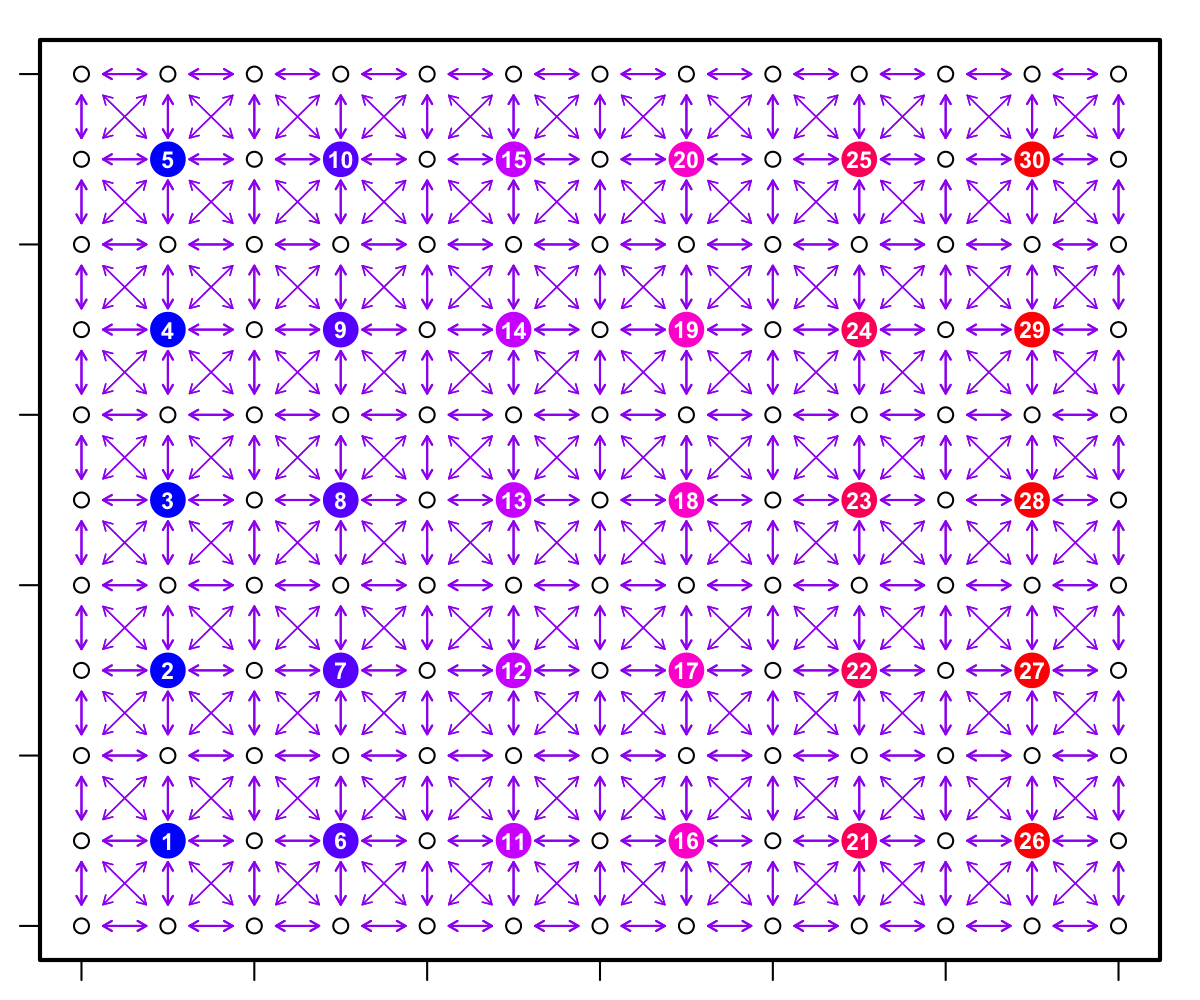
\includegraphics[width=2.8in,height=2.33in]{figs/sims/basic_lattice.png}}
		\subcaptionbox{Lattice \label{lattice_inference}}
			{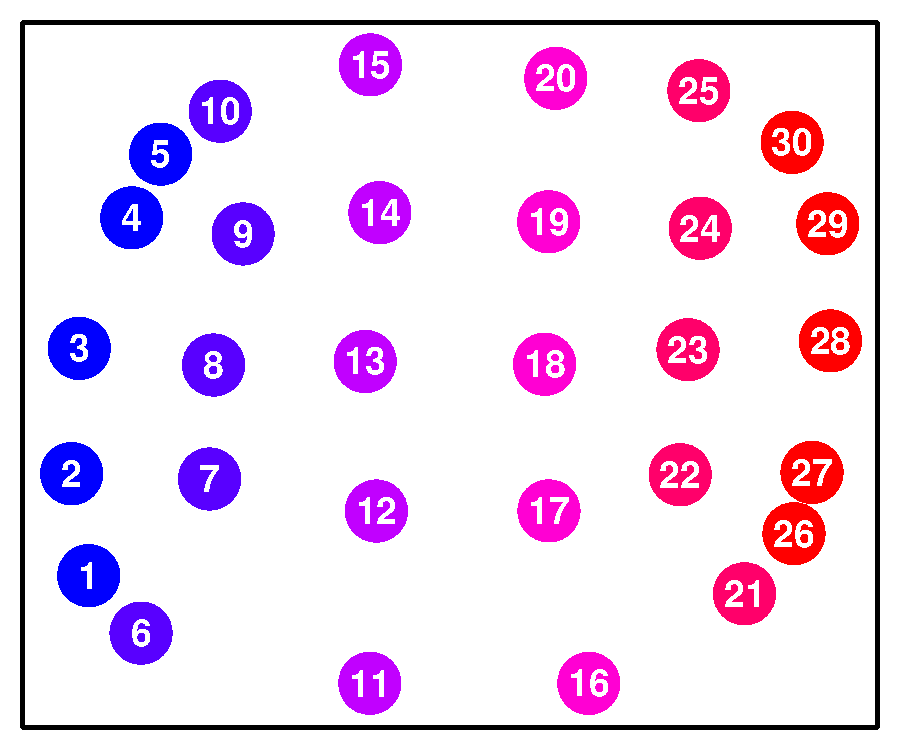
\includegraphics[width=2.8in,height=2.33in]{figs/sims/GeoGenMap_lattice.pdf}}
		\subcaptionbox{Barrier \label{barrier_inference}}
			{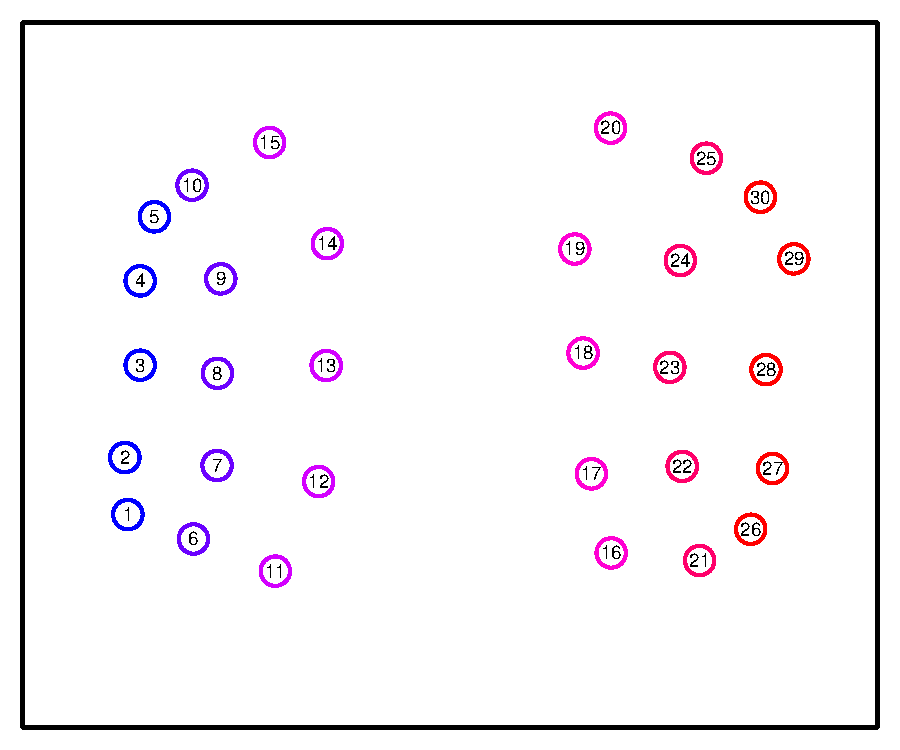
\includegraphics[width=2.8in,height=2.33in]{figs/sims/GeoGenMap_barrier.pdf}}
		\subcaptionbox{Expansion  \label{expansion_inference}}
			{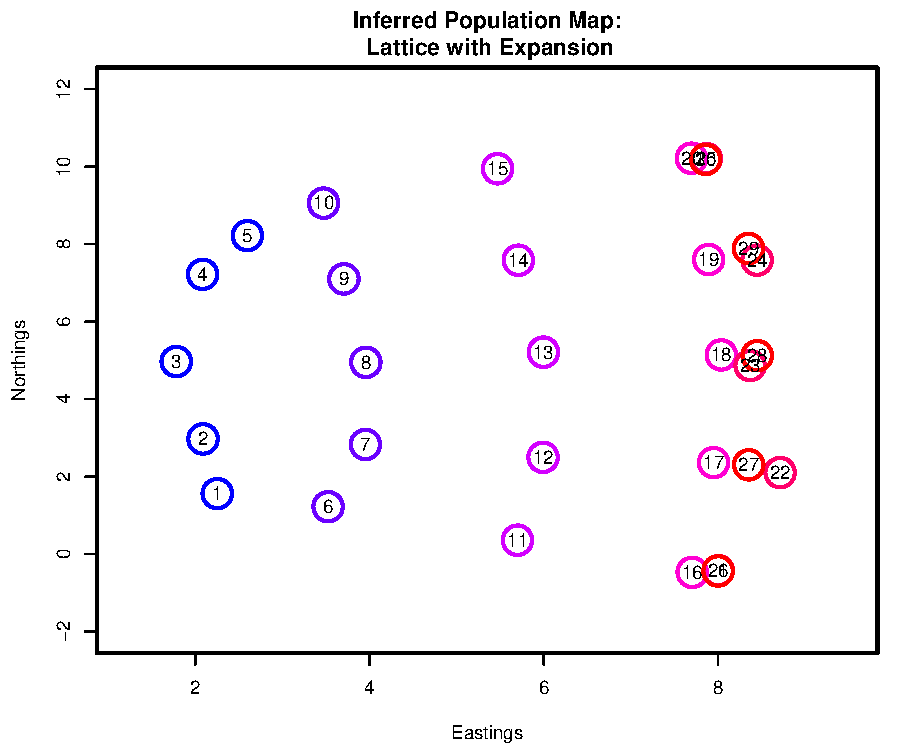
\includegraphics[width=2.8in,height=2.33in]{figs/sims/GeoGenMap_expansion.pdf}}
	\caption{Population maps inferred using SpaceMix under three different scenarios: a) configuration of simulated populations; (c) simple lattice at equilibrium; c) a lattice with a barrier across the center line of longitude; d) a lattice with recent expansion on the eastern margin.}\label{sfig:lattice_scenarios}
\end{figure}


\begin{figure}
	\centering
		\subcaptionbox{Location Inference \label{sfig:admixture_inference_CYOL}}
			{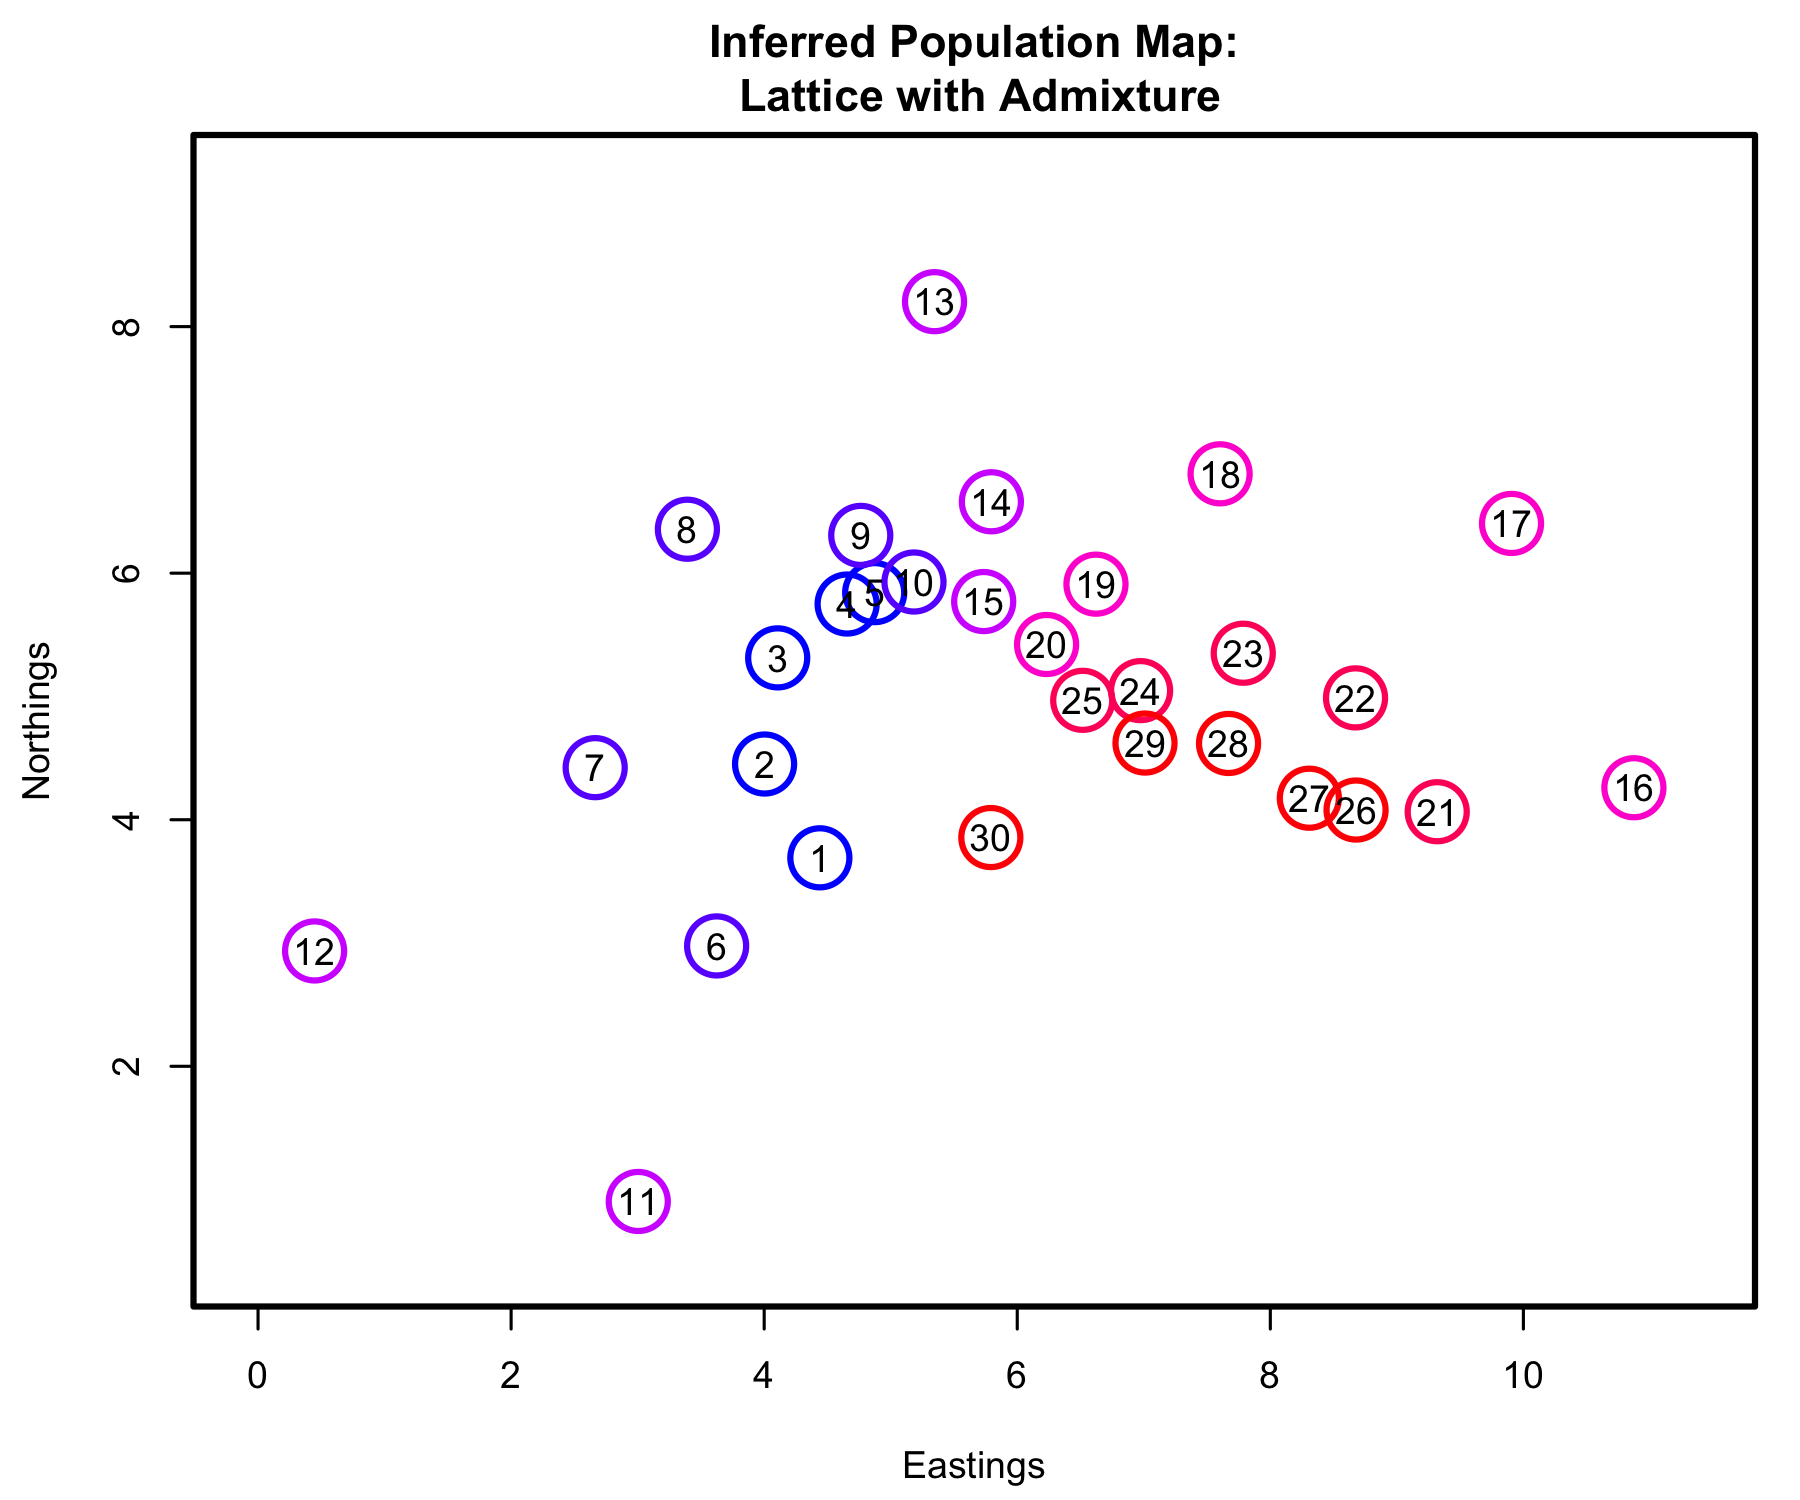
\includegraphics[width=2.4in,height=2in]{figs/sims/GeoGenMap_corner_admixture_CYOL.png}}
		\subcaptionbox{Location and Admixture Inference \label{sfig:admixture_inference_CYOL}}
			{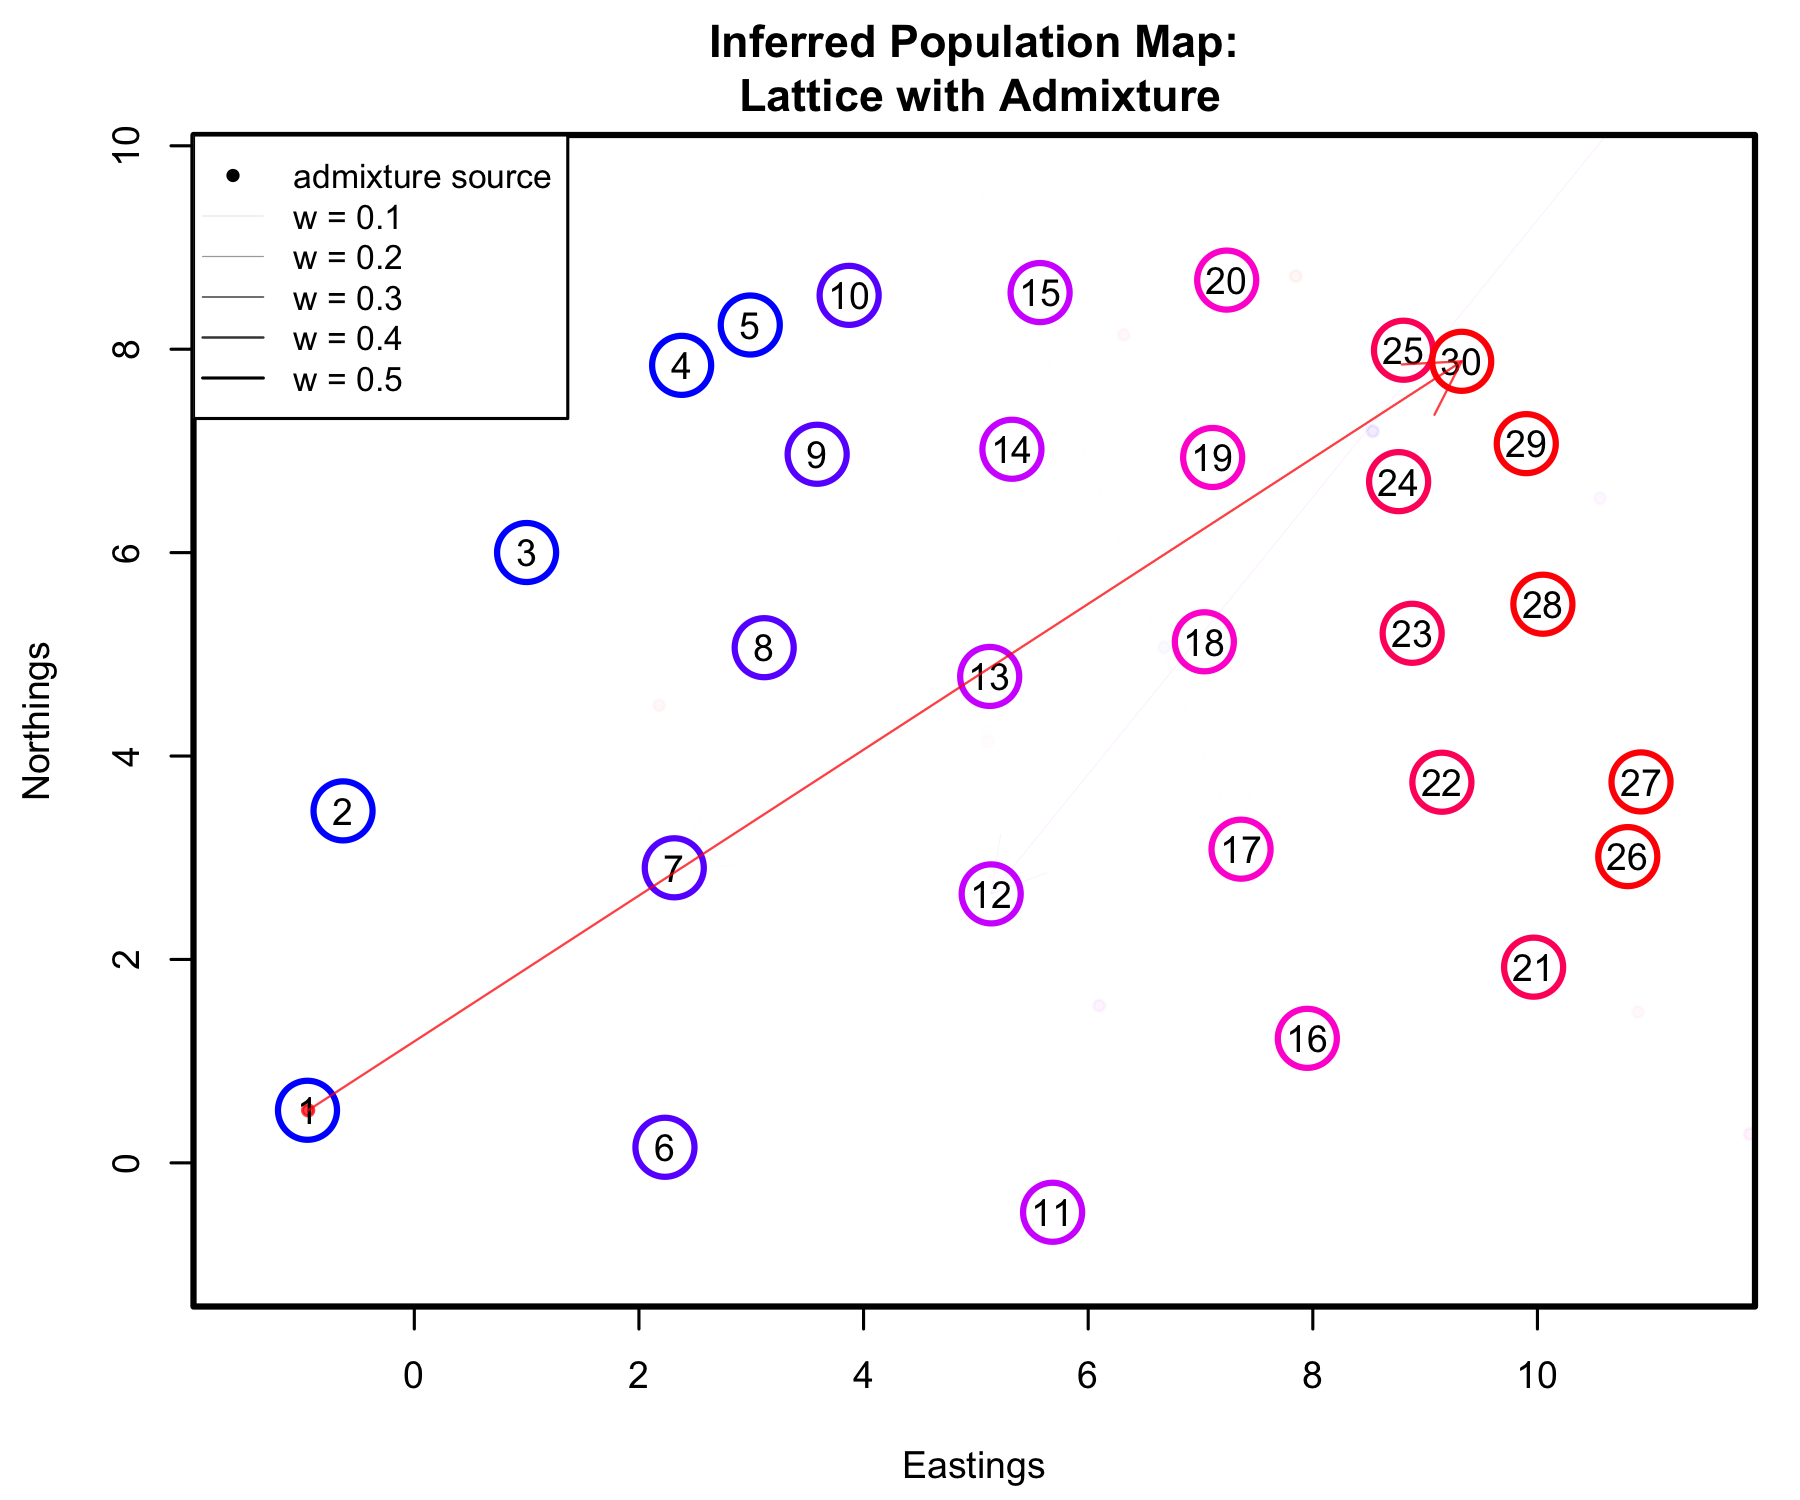
\includegraphics[width=2.4in,height=2in]{figs/sims/GeoGenMap_corner_admixture.png}}
	\caption{Inference of population locations in the scenario depicted in Figure \ref{sfig:admixture_scenario}.  Population 30 has received half of its lineages from population 1, to simulate a long distance admixture event in the very recent past. a) Inference of population locations; b) inference of both population locations and their sources of admixture}\label{sfig:corner_admixture_inference}
\end{figure}


To examine the behavior of SpaceMix when there is long distance covariance between populations, we simulated an admixture event on the stepping-stone model we had used previously.  Specifically, (using Fig. \ref{sfig:lattice_scenarios}\subref{simple_lattice} as a reference) we allowed population 30, in the northeast corner of the grid, to draw half of its ancestry from population 1, in the southwest corner.  The result of a SpaceMix analysis in which the locations of these populations were estimated is shown in Figure \ref{sfig:corner_admixture_inference}\subref{admixture_inference_CYOL}.
This signal of excess covariance over anomalously long distances is clearly difficult to accommodate within the ``choose-your-own-location" framework described above.  In Figure \ref{sfig:corner_admixture_inference}\subref{admixture_inference_CYOL}, the reader can see the torturous lengths to which the method goes to come up with a configuration of populations that accommodates their genetic relationships.  The admixed population 30 is estimated to have a location intermediate between population 1, the source of its admixture, and populations 24, 25, and 29, the nearest neighbors to the location of its non-admixed lineages.  However, this warping of space is difficult to interpret, especially in the visualization of genetic relationships in empirical data for which a researcher does not know the true demographic history.  It would therefore be of great utility to directly model the action of admixture on spatial patterns of genetic variation.

%%%%%%%%% %%%%%%%%% 
\subsection*{Inference of Spatial Admixture}
We can incorporate recent admixture directly into out inference framework.  We imagine that population $k$ draws the majority of its ancestry from $G_{k'}$, but a proportion $0 \geq w_k \leq 0.5$ of its ancestry comes from another location \kadmixsource{k}, which we refer to as its source of admixture. The mean standardized population allele frequency at locus $\ell$ in population $k$ is a weighted average of the allele frequencies at the geographic location of the sampled population chooses for itself ($p_{\ell,k'}$) and those at the coordinates of the source ($p_{\ell,\identifyadmixsource{k}}$) from which the observed population draws admixture:
\begin{equation}
w_k p_{\ell,k'} + (1-w_k) p_{\ell,\identifyadmixsource{k}} \label{eqn-admixedfreq}
\end{equation}
We can allow each of our populations to have an independent spatial source of admixture. Our $p_{\ell,k'}$ and $p_{\ell,\identifyadmixsource{k}} $ are well defined, as, given our population allele frequency covariance matrix, Eqn. \ref{eq:spatial_covariance}, we can get the distribution of allele frequencies at any point in space simply by plugging its spatial coordinates into our $\Omega(D(G))$.

%where $p_{\ell,k}$ are the model-estimated allele frequencies at locus $\ell$ at the spatial location of population $G_k$ and $p_{\ell,k*}$ are the model-estimated allele frequencies at the spatial location of the source of admixture \kadmixsource{k}. 

We can then consider the resulting parametric covariance matrix that follows from the form of the population frequencies in Eqn. \eqref{eqn-admixedfreq}. The covariance between the standardized allele frequencies of population $i$ and $j$ can be modeled as 
\begin{alignat}{3}
\label{eq:admixed_covariance_1}
\Omega_{i,j}^{(*)} = (1-w_i)(1-w_j) \Omega_{i\;,\;j\;} \; \times&\\
(w_i)(1-w_j) \Omega_{\identifyadmixsource{i},\;j\;} \; \times   \notag&\\
(w_j)(1-w_i) \Omega_{i\;,\;\identifyadmixsource{j}} \; \times   \notag&\\
(w_i)(w_j) \Omega_{\identifyadmixsource{i},\;\identifyadmixsource{j}} \; +   \notag&\\
\delta_{i,j} (\eta_i + \bar{S}^{-1}) \notag&
\end{alignat}
where $\identifyadmixsource{i}$ and $\identifyadmixsource{j}$ are the sources from which populations $i$ and $j$ are drawing their admixture with proportions $p_i$ and $p_j$, and the spatial covariance function of population frequencies, $\Omega$, is given by \eqref{eq:spatial_covariance} (this lacks the sample-specific variance terms on the diagonal). Note that we then reintroduce the nugget, $\eta_i$, and the sample size effect, $\bar{S}^{-1}$, for each population, to model drift or excess variance in population $i$ on top of that predicted by the mixture of frequencies predicted by our spatial model.  As in Eqn. \eqref{eq:spatial_covariance2}, $\delta_{i,j} $ is the indicator function $1$ if $i=j$, and $0$ otherwise. 

%parameterized by the pairwise geographic distances between each pair of populations, \emph{without} the population-specific variance terms on the diagonal (i.e., in Eqn. \eqref{eq:admixed_covariance_1}, i.e. $\Omega_{i,j} = \frac{1}{\alpha_0} \text{exp} \left(	\left( \alpha_1D_{i,j} \right)^{\alpha_2} \right)$).  

The admixed covariance between samples $i$ and $j$, $\Omega_{i,j}^{(*)}$ is then a function of all the pairwise spatial covariances between populations $i$ and $j$ and the points from which they draw admixture, $\identifyadmixsource{i}$ and $\identifyadmixsource{j}$.  Those spatial covariances in turn are a function of all combinations of pairwise distances between their locations: $G_i$, $G_i$, \kadmixsource{i}, and \kadmixsource{j}.  This parametric covariance form is illustrated in Figure \ref{sfig:admixed_cov_diagram}.

As we only get to observe the sample frequencies and we standardize our allele frequencies using the sample mean, our predicted admixture covariance matrix needs to be transformed to accommodate these sampling considerations. We can do this as before (see methods XXXX), and we again treat the likelihood of our sample covariance matrix as Wishart:
\begin{equation}
\label{eq:wishart_dist_admixed}
P(\widehat{\Omega} \mid \identifyadmixsource{\Omega}) = 
	\mathcal{W}\left(\widehat{\Omega} \mid L^{-1} \identifyadmixsource{\Omega} \left( G',\identifyadmixsource{G}, \vec{w},\vec{\alpha}\right),L \right)	\text{.}
\end{equation}
As before $G'$, $\vec{\alpha}$, $\vec{\eta}$ are treated as random variables to be estimated. Now the set of $K$ admixture sources $\identifyadmixsource{G}$ are also parameters to be estimated, along with the vector of $K$ admixture proportions $\vec{w}$. The posterior probability of these parameters can be expressed as a function of this parametric admixed covariance, $\identifyadmixsource{\Omega}$,
\begin{equation}
\label{eq:admixed_post_prob}
P(G',\identifyadmixsource{G}, \vec{p},\vec{\alpha}, \eta \mid \widehat{\Omega}, L,G) 
	\propto  
		P(\widehat{\Omega}  \mid \identifyadmixsource{\Omega}) P(\vec{\alpha}) P(G') P(\identifyadmixsource{G}) P(\vec{w}) P(\eta) 
\end{equation}
%
as specified by the parameters $w$, $\identifyadmixsource{G}$, $\vec{\alpha}$, and $\eta$, and the observed locations, $G$.  We place the same priors as stated above on $\vec{\alpha}$, $\eta$, and we now specify priors on $q$ and $\identifyadmixsource{G}$.  The admixture proportions, $w$, are capped at 0.5, to prevent populations from swapping identities with their source of admixture, and are heavily weighted towards small values to be conservative with respect to admixture inference.  Our admixture proportions are independently beta-distributed: $2 w_k \sim \beta(\alpha = 1,\beta = 100)$.  The priors on the sources of admixture, $\identifyadmixsource{G}$ are taken independently as bivariate normal spatial distributions, all with the same mean at the centroid of the observed population locations, $G$, and variance equal to twice the mean pairwise observed distance:  $\identifyadmixsource{G_k} \sim \mathcal{N}(\mu = \bar{G},\sigma = 2 \bar{D}(G))$.


%We treat the location of the source of admixture for population $k$, $\identifyadmixsource{G_k}$, and the population's admixture proportion, $p_k$, as random variables and jointly estimate them as part of our inference procedure. 

The models described above may be used in various combinations.  In the simplest model, populations may not choose their own locations, nor are they allowed to draw admixture, and the only parameters to be estimated are those of the spatial covariance function given in Eqn \eqref{eq:spatial_covariance}, and the population-specific variance terms ($\eta_k$).  In the most complex model, population locations, the locations of their sources of admixture, and the proportions of that admixture are all estimated jointly in addition to the parameters of the spatial covariance function and the population specific variances.  %The full likelihood of this most complex parameterization is given by,

An natural concern is whether all of these parameters are separately identifiable, most notability whether population locations, admixture locations and proportions can be estimated. If a population has received some level of admixture from a another population what is to stop it simply moving towards that population in geogenetic space to satisfy its increased resemblance to that population, rather than choosing admixture from that location. The recent developments to test for admixture from population allele frequencies \citep{treemix}, rely on the fact that a population tree dictates particular conditions on the covariances of allele frequency differences among particular parts of the tree. Violations of these conditions allow for admixture to be identified, and also highlight conditions under which these tests may be misled (ancient population structure). Similarly admixture is identifiable in our model as their are covariance relationships among populations that can not simply be satisified by shifting populations locations around (as demonstrated by the tortured nature of Figure \ref{sfig:admixture_inference_CYOL}). To illustrate this point consider the simple spatial admixture scenerio shown in Figure \ref{fig:toy_admixture}. Our populations A-D are arrayed spatially along a line, and there allele frequencies are specified by a simple isolation by distance model. The lines show the expected covariance that a population at a given distance to populations A, B, or D (as indicated by line color). There is recent admixture from D into B (such that 40\% of the alleles in B are drawn from D). The dots show the resulting admixed covariance between B and the three other populations, as well as B's variance (B-B) as specified by equation \eqref{eq:admixed_covariance_1}, with no nugget or sampling effect
\begin{figure}[ht!]
	\centering
	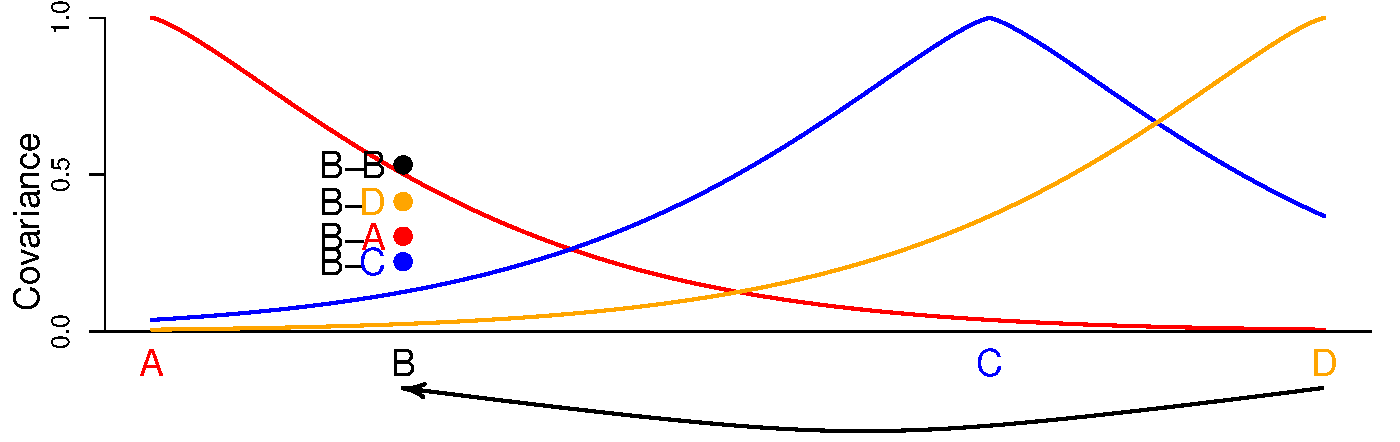
\includegraphics[width=\textwidth]{figs/Admix_covar_toy_fig.pdf}
	\caption{} \label{fig:toy_admixture}
\end{figure}
Due to the admixture B has lower covariance with A than expected given its distance, somewhat higher covariance with C, and much higher covariance with D. In addition the variance of B is lower than the other three populations, which each have variance $1$, the value of covariance when the distance is zero. This lower variance results from the fact that the frequencies at $B$ represent a mixture of the frequency at $D$ and the frequency at $B$ before the admixture. For the sake of simplicity lets assume that we hold the locations of A, B, and D constant, as well as the decay of covariance with distance (as could be the case if A-D are part of a larger analysis).  The covariance relationships of $B$ to the other populations can not be simply satisfied by moving $B$ towards D. Doing so would better match B's covariance to D, but it would then have to covary much more with C and much less with A than we observe. Moving B also does not resolve its lower variance than the other populations. Introducing admixture into the model allows it to satisify all of these conditions, it can draw ancestry from D but keep part of its resemblance to A, it also avoids B having to closer to C. Even in the absence of a sample from population C, B's covariance with A and D and its low variance could not be satisfied simply by moving B. B is better described as a linear mixture of a population close to A and D.


%%%Graham's attempts at arrows in equations
%\begin{equation}
%\source{A}~~~~B~~~~ \target{C}~~~~D
%\drawarrows
%\end{equation}
%blah blah

% \begin{equation}
%   A~~~~B\tikzmark{b} ~~~~ C~~~~\tikzmark{a}D
%   \tikz[overlay,remember picture]
%    {\draw[->,square arrow] (a.south) to (b.south);}
% \end{equation}
% blah blah
% \begin{equation}
%   A~~~~B\tikzmark{b} ~~~~ C~~~~\tikzmark{a}D
%   \tikz[overlay,remember picture]
%    {\draw[->,square arrow] (a.south) to (b.south);}
% \end{equation}
 
 
%\newcommand{\tikzmark}[1]{\tikz[overlay,remember picture] \node (#1) {};}
%\tikzset{square arrow/.style={to path={-- ++(0,-.25) -| (\tikztotarget)}}}

%\begin{equation}
 % a\tikzmark{a}x^2 + bx + c = 5\tikzmark{b}x^2 + bx + c.
 % \tikz[overlay,remember picture]
 %  {\draw[->,square arrow] (a.south) to (b.south);}
%\end{equation}
 


Using the example admixture scenario described above and used in the analysis depicted in Figure \ref{sfig:admixture_inference_CYOL}, we demonstrate the inference of populations' sources and strengths of admixture and illustrate the results in Figure \ref{sfig:corner_admixture_just_adinf}.  The reader can see that only the admixed population (population 30) is drawing admixture from the location of the source of admixture that was used to simulate the data, and that all other populations, which are not admixed, are choosing to draw admixture in only negligible amounts. \gc{run with choose your own location + admixture.

\begin{figure}[ht!]
	\centering
	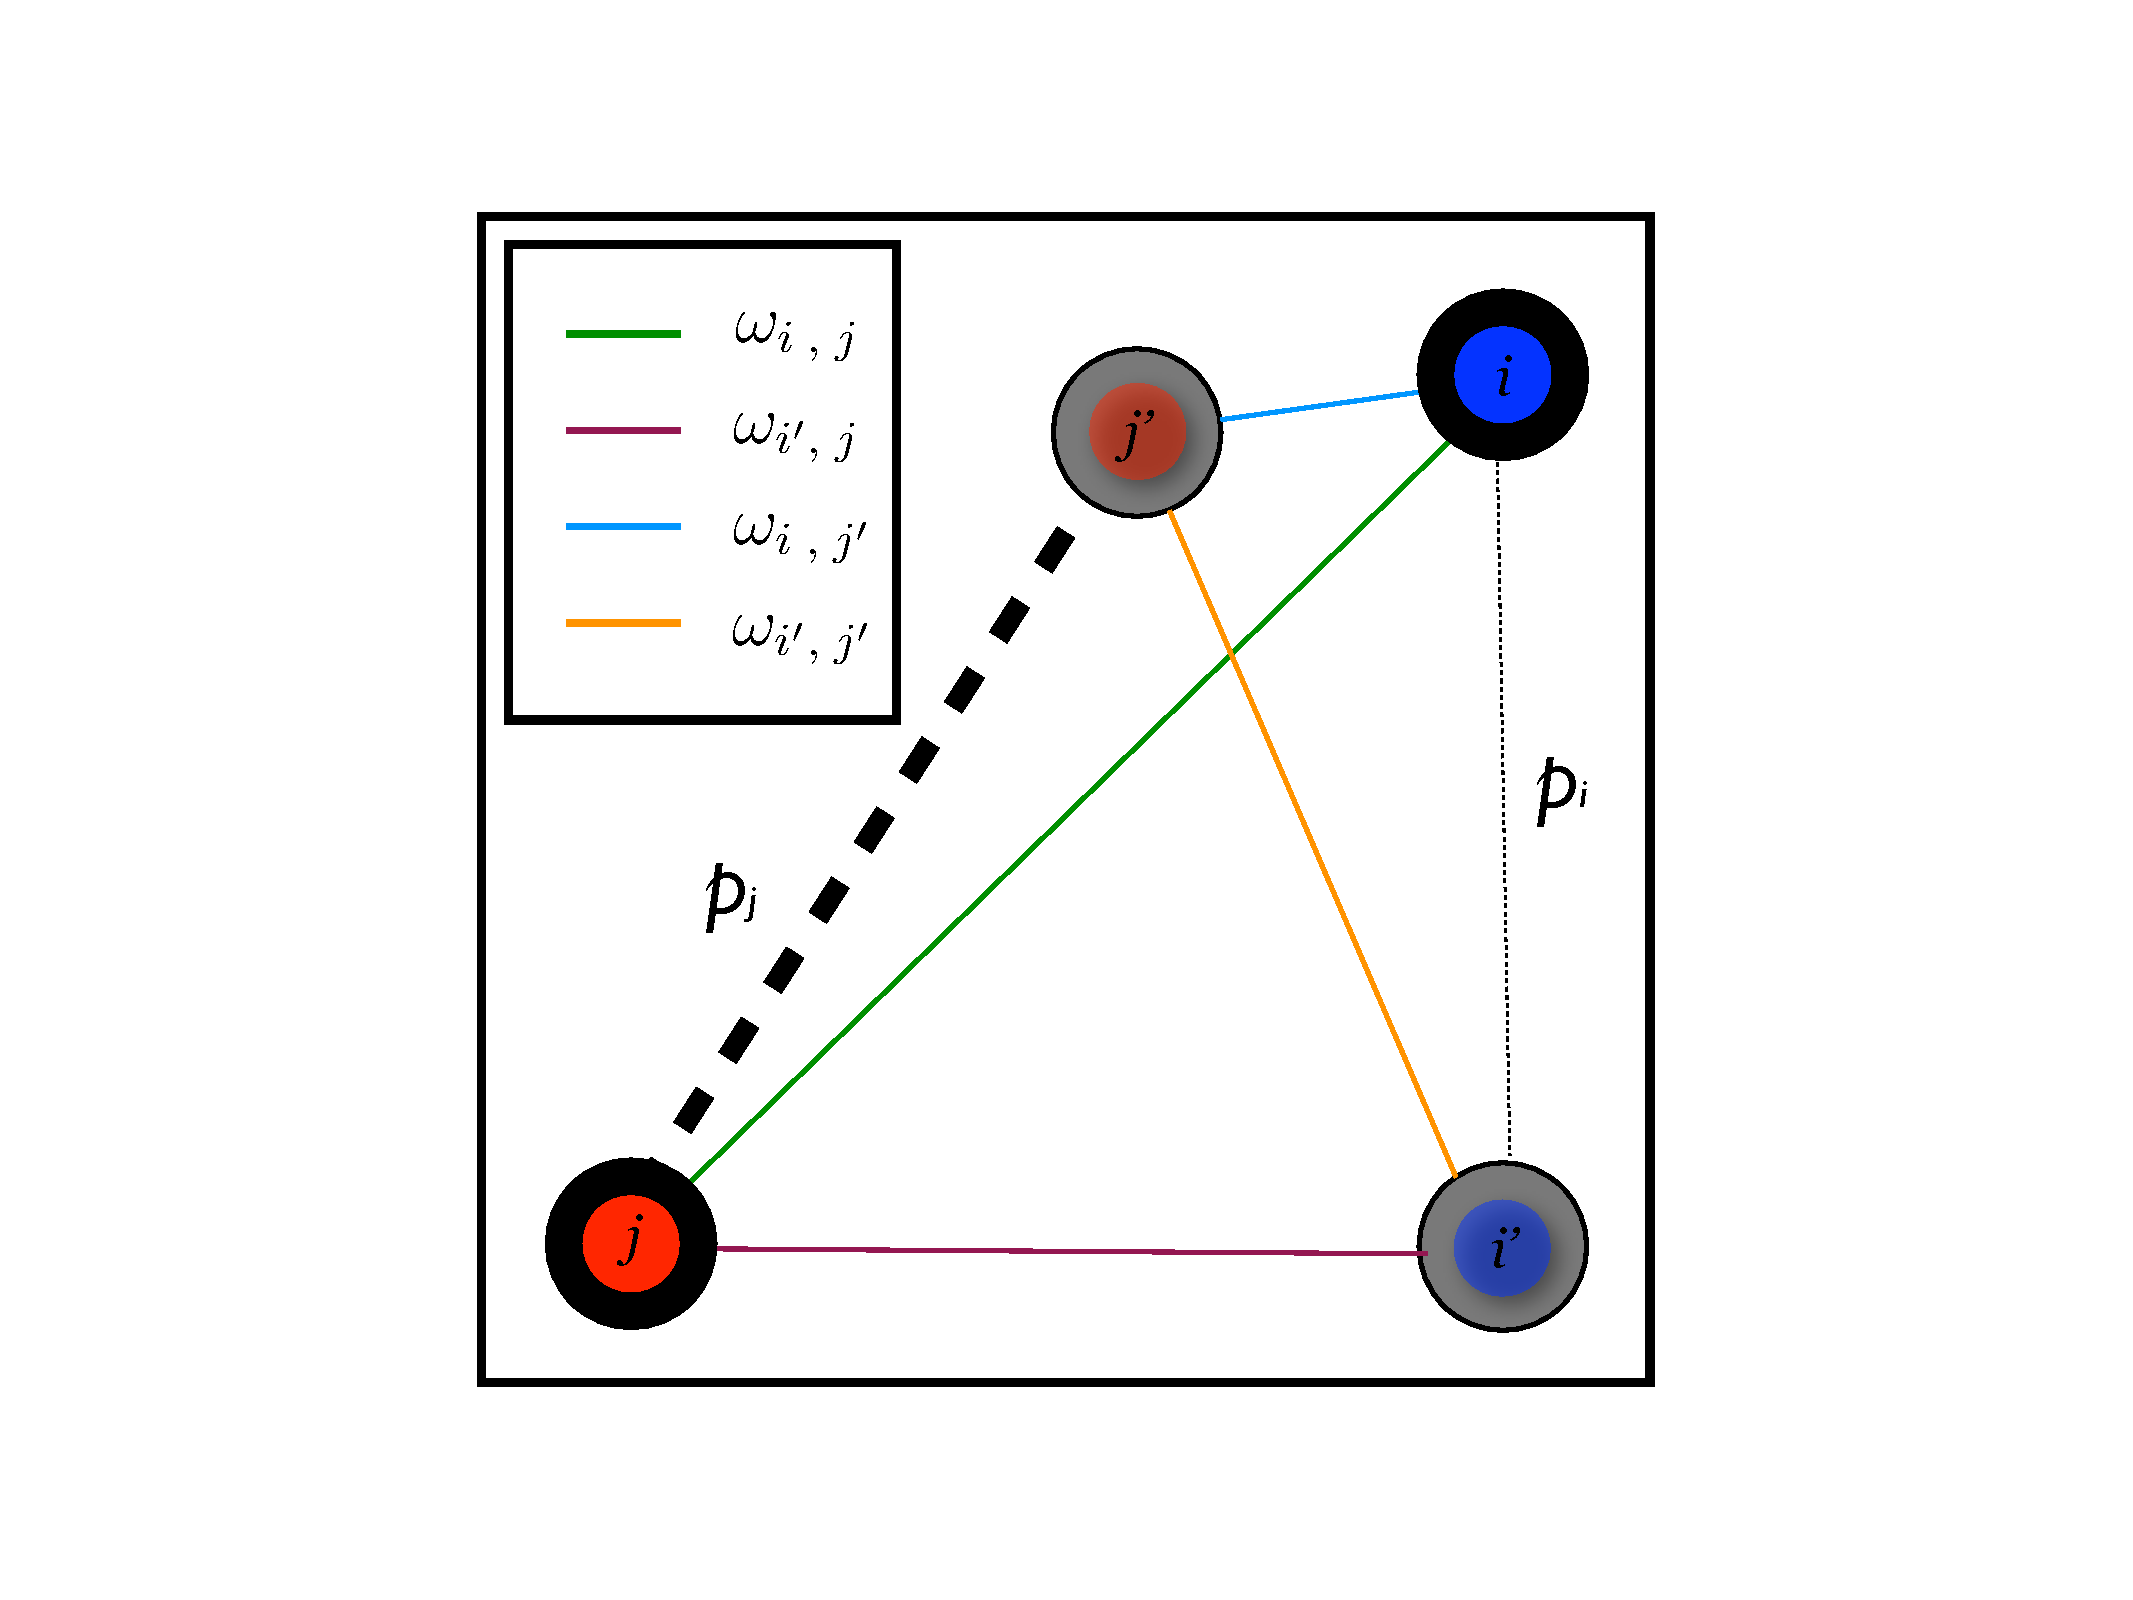
\includegraphics[width=2in,height=2in]{figs/admix_cov_fig.pdf}
	\caption{An illustration of the form of the admixed covariance given in Eqns. \eqref{eq:admixed_covariance_1} and \eqref{eq:admixed_covariance_2}.  Populations $i$ and $j$ are drawing admixture in proportions $p_i$ and $p_j$ from their respective sources of admixture, $i^{(*)}$ and $j^{(*)}$, and all pairwise spatial covariances (the $\Omega$'s) are shown.  In this cartoon example, population $j$ is drawing more admixture from its source $j^{(*)}$ than $i$ is from its source $i^{(*)}$ (i.e., $p_j > p_i$).}\label{sfig:admixed_cov_diagram}
\end{figure}


\begin{figure}[ht!]
	\centering
	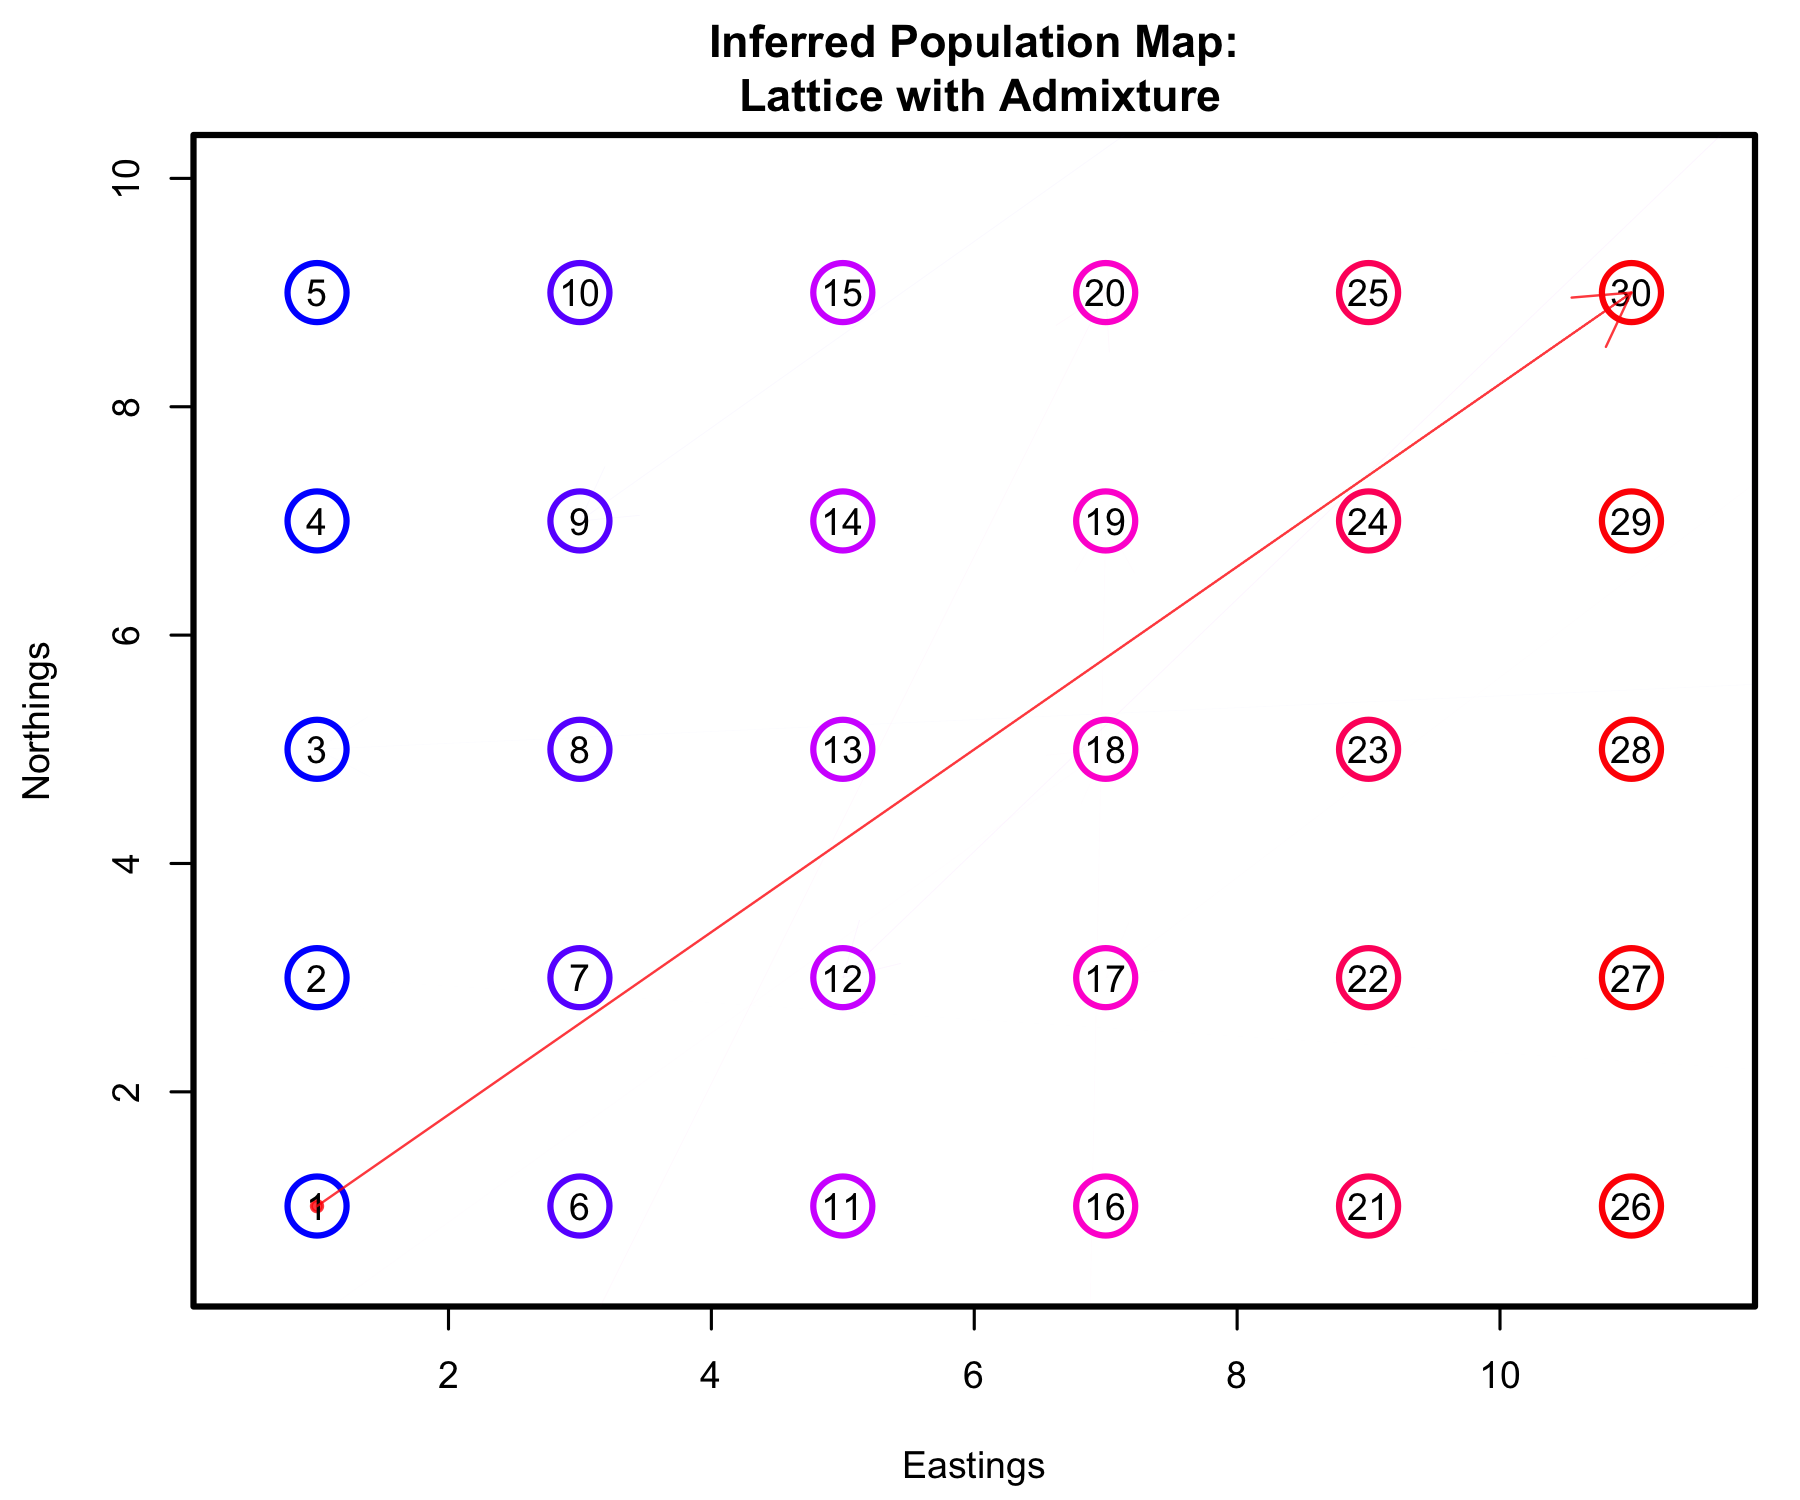
\includegraphics[width=2.4in,height=2in]{figs/sims/GeoGenMap_corner_admixture_adinf.png}
	\caption{Posterior distribution of inference of the sources and strengths of admixture for the sampled populations.  The admixed population (Population 30) is drawing admixture from the location of its source of admixture that was used to simulate the data (the location of Population 1).}\label{sfig:corner_admixture_just_adinf}
\end{figure}

%\subsection*{Models}

%\begin{equation}
%\label{eq:wishart_dist_admixed}
%P(\widehat{\Omega} \mid \identifyadmixsource{\Omega}) = 
%	\mathcal{W}\left(\widehat{\Omega} \mid L^{-1} \identifyadmixsource{\Omega} \left( G',\identifyadmixsource{G}, \vec{p},\vec{\alpha}\right),L \right)	\text{.}
%\end{equation}

%Now, the posterior probability can be expressed as a function of this parametric admixed covariance, $\identifyadmixsource{\Omega}$,
%\begin{equation}
%\label{admixed_post_prob}
%P(G',\identifyadmixsource{G}, \vec{p},\vec{\alpha}, \eta \mid \widehat{\Omega}, L,G) 
%	\propto  
%		P(\widehat{\Omega}  \mid \identifyadmixsource{\Omega}) P(\vec{\alpha}) P(G') P(\identifyadmixsource{G}) P(\vec{p}) P(\eta) 
%\end{equation}
}

To demonstrate the use of the model in which the location of each population as well as the location of its source of admixture are estimated jointly, we used the spatial stepping-stone coalescent simulation procedure described above to generate a dataset of populations on a lattice in which there is both a barrier to dispersal and a more subtle admixture event (admixture proportion = 10\%, see Fig. \ref{sfig:barr_inland_ad}\subref{barr_inland_ad_scenario}).  In the SpaceMix analysis (Fig. \ref{sfig:barr_inland_ad}\subref{barr_inland_ad_inference}), the separation of the east and west sides of the grid accommodates the effect of the barrier to migration, and the admixed population (population 23) chooses admixture from very close to its true source (population 13), and in close to the correct amount ($\bar{p} = 0.05; 95\% \text{ credible interval} = 0.02-0.08$). \gb{discuss how prior forces amount down, so it's cheaper to choose more westward pop as source}.

\begin{figure}[ht!]
	\centering
		\subcaptionbox{Lattice \label{barr_inland_ad_scenario}}
			{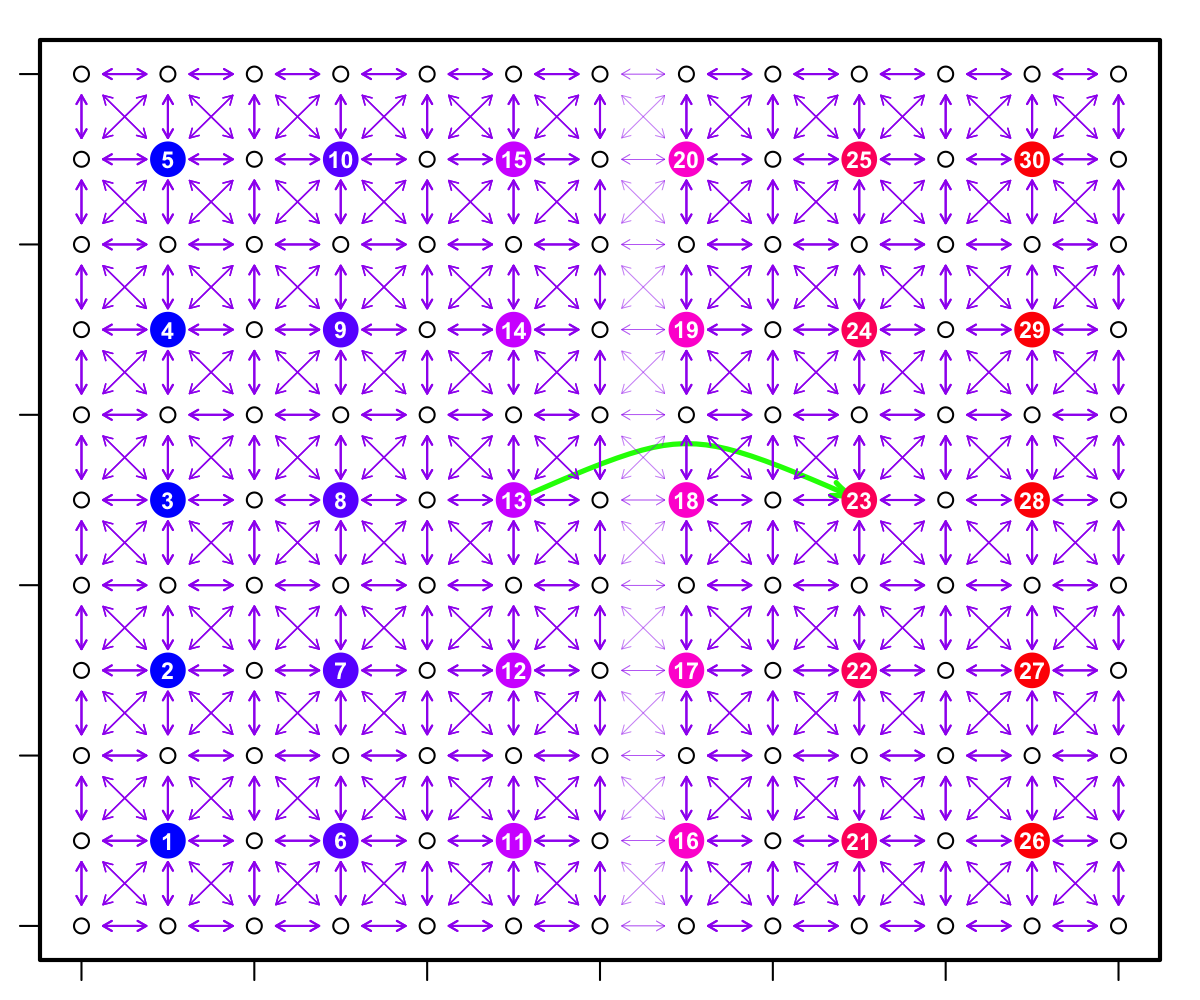
\includegraphics[width=2in,height=1.66in]{figs/sims/barr_indland_ad_lattice.png}}
		\subcaptionbox{Barrier \label{barr_inland_ad_inference}}
			{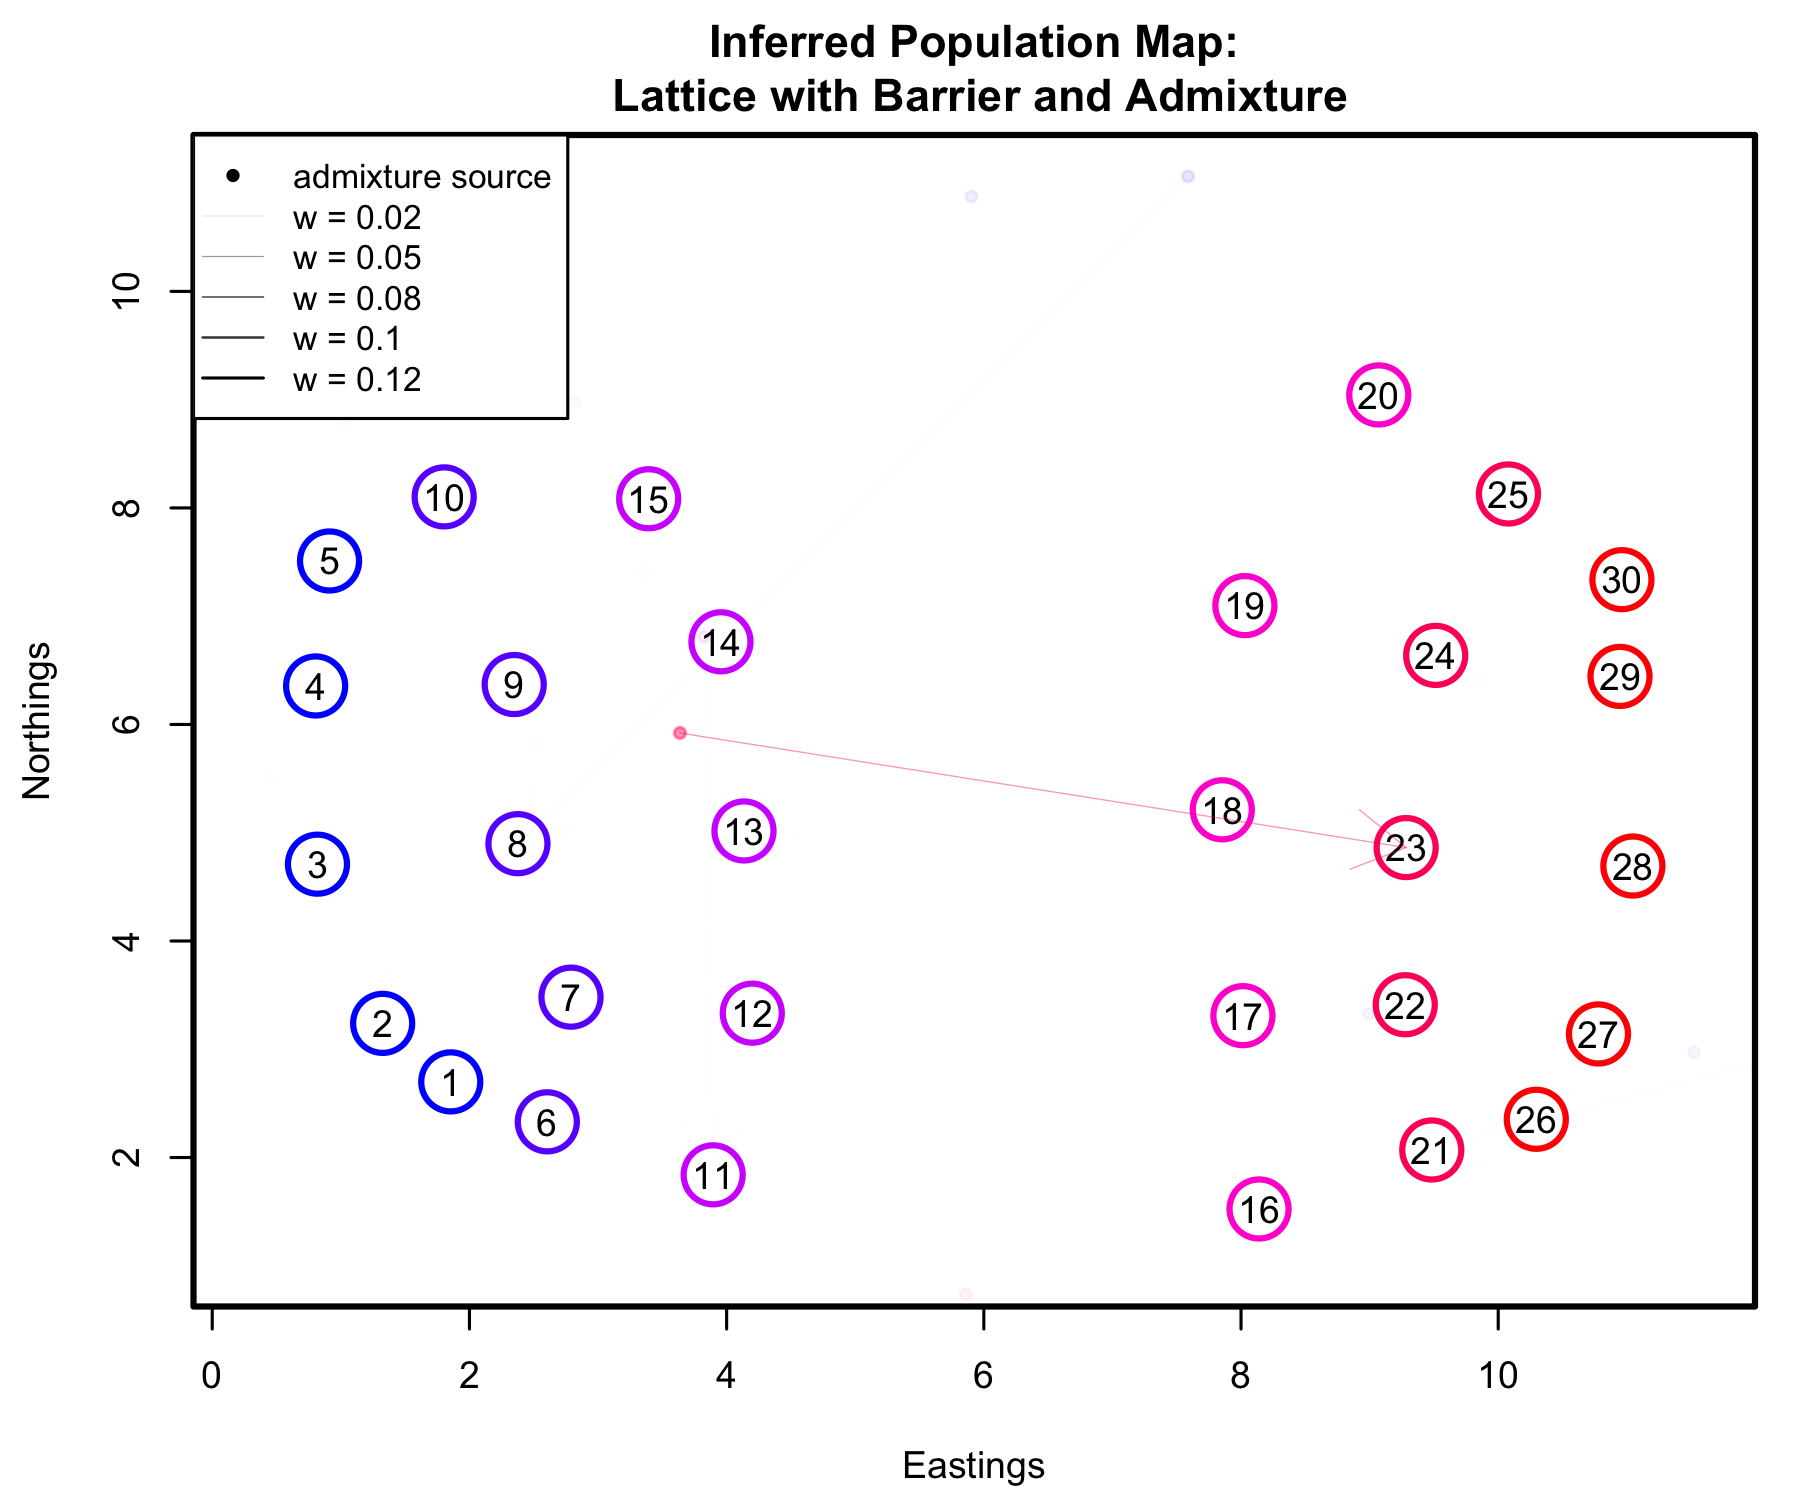
\includegraphics[width=2in,height=1.66in]{figs/sims/GeoGenMap_barr_inland_admixture_1.png}}
	\caption{Population maps inferred using SpaceMix under three different scenarios: a) simple lattice at equilibrium; b) a lattice with a barrier across the center line of longitude; c) a lattice with recent expansion on the eastern margin.}\label{sfig:barr_inland_ad}
\end{figure}
%This most complex model is, in many cases, nonetheless identifiable.  Although in certain scenarios, a population may choose a location nearer to its source of admixture, rather than 

\section*{Empirical Applications}
To demonstrate the applications of this novel method, we analysed population genomic data from two systems: the greenish warbler ring species complex, and a global sampling of contemporary human populations.

\subsection*{Greenish Warblers}  
The greenish warbler (\emph{Phylloscopus trochiloides}) species complex is broadly distributed around the Tibetan plateau, and exhibits gradients around the ring in a range of phenotypes including song, as well allele frequencies (Ticehurst (1938),Irwin et al 2001, Irwin et al 2005, Irwin et al 2008).  At the northern end of the ring in central Siberia, where the eastern and western arms of population expansion meet, there are discontinuities in call and morphology, as well as a genetic discontinuity and reproductive isolation (Irwin et al 2001, Irwin et al 2008). It is proposed that the species complex represents a ring species, in which selection and/or drift, acting in the populations as they spread northward on either side of the Tibetan plateau, have led to the evolution of reproductive isolation (REFs).  The question of whether it constitutes a ring species, in purest form, focuses on whether gene flow along the margins of the plateau has truly been continuous throughout the history of the expansion or if, alternatively, discontinuities in migration around the species complex's range have facilitated periods of differentiation in genotype or phenotype without gene flow (Mayr 1942, Mayr 1970, Coyne and Orr 2004).  However, we note that many would still classify this as a ring species even if that condition were not met, just not as a case of speciation-by-distance \citep[see][ for discussion]{}.


\gc{Based on a larger SNP dataset Alcaide et al (2014),} have suggested that the greenish warbler species complex constitutes a `broken' ring species, in which there have been historical discontinuities in gene flow that facilitated the evolution of reproductive isolation between adjacent forms.  Because the questions in this system are fundamentally both geographic and genetic in nature, it is eminently SpaceMix-able, and, within this spatial framework, we performed a number of analyses to investigate the geographic context of population differentiation in the greenish warbler species complex. For these analyses, we used the dataset from Alcaide et al (2014), which consisted of 95 individuals sampled at 22 distinct locations and sequenced at 2,334 SNPs, of which 2,247 were bi-allelic and retained for SpaceMix runs. 

\begin{figure}
	\centering
		\subcaptionbox{Warbler subspecies distribution map \label{irwin_map}}
			{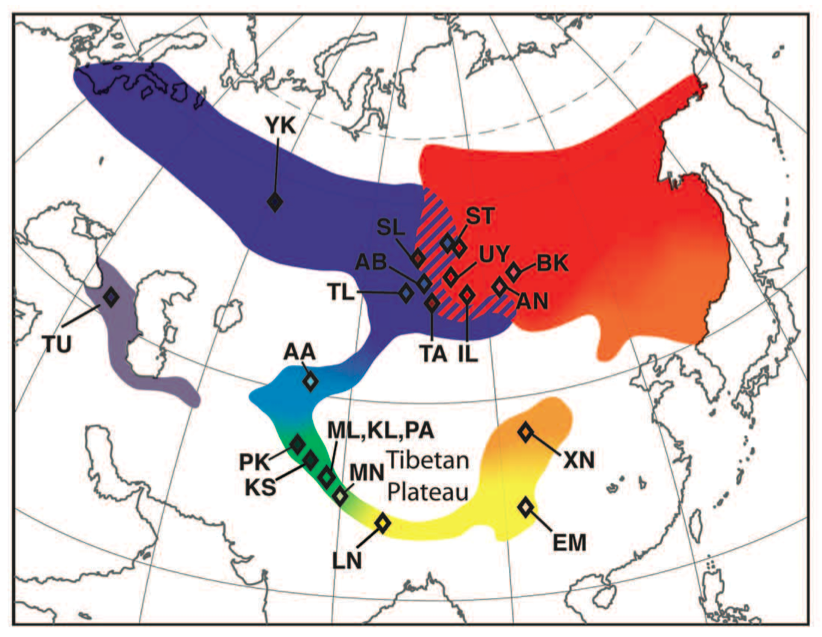
\includegraphics[width=2.4in,height=2in]{figs/warblers/Irwin_warbler_map_figure.png}}
		\subcaptionbox{Inferred admixture proportions and population nuggets \label{warb_pop_adnug}}			
			{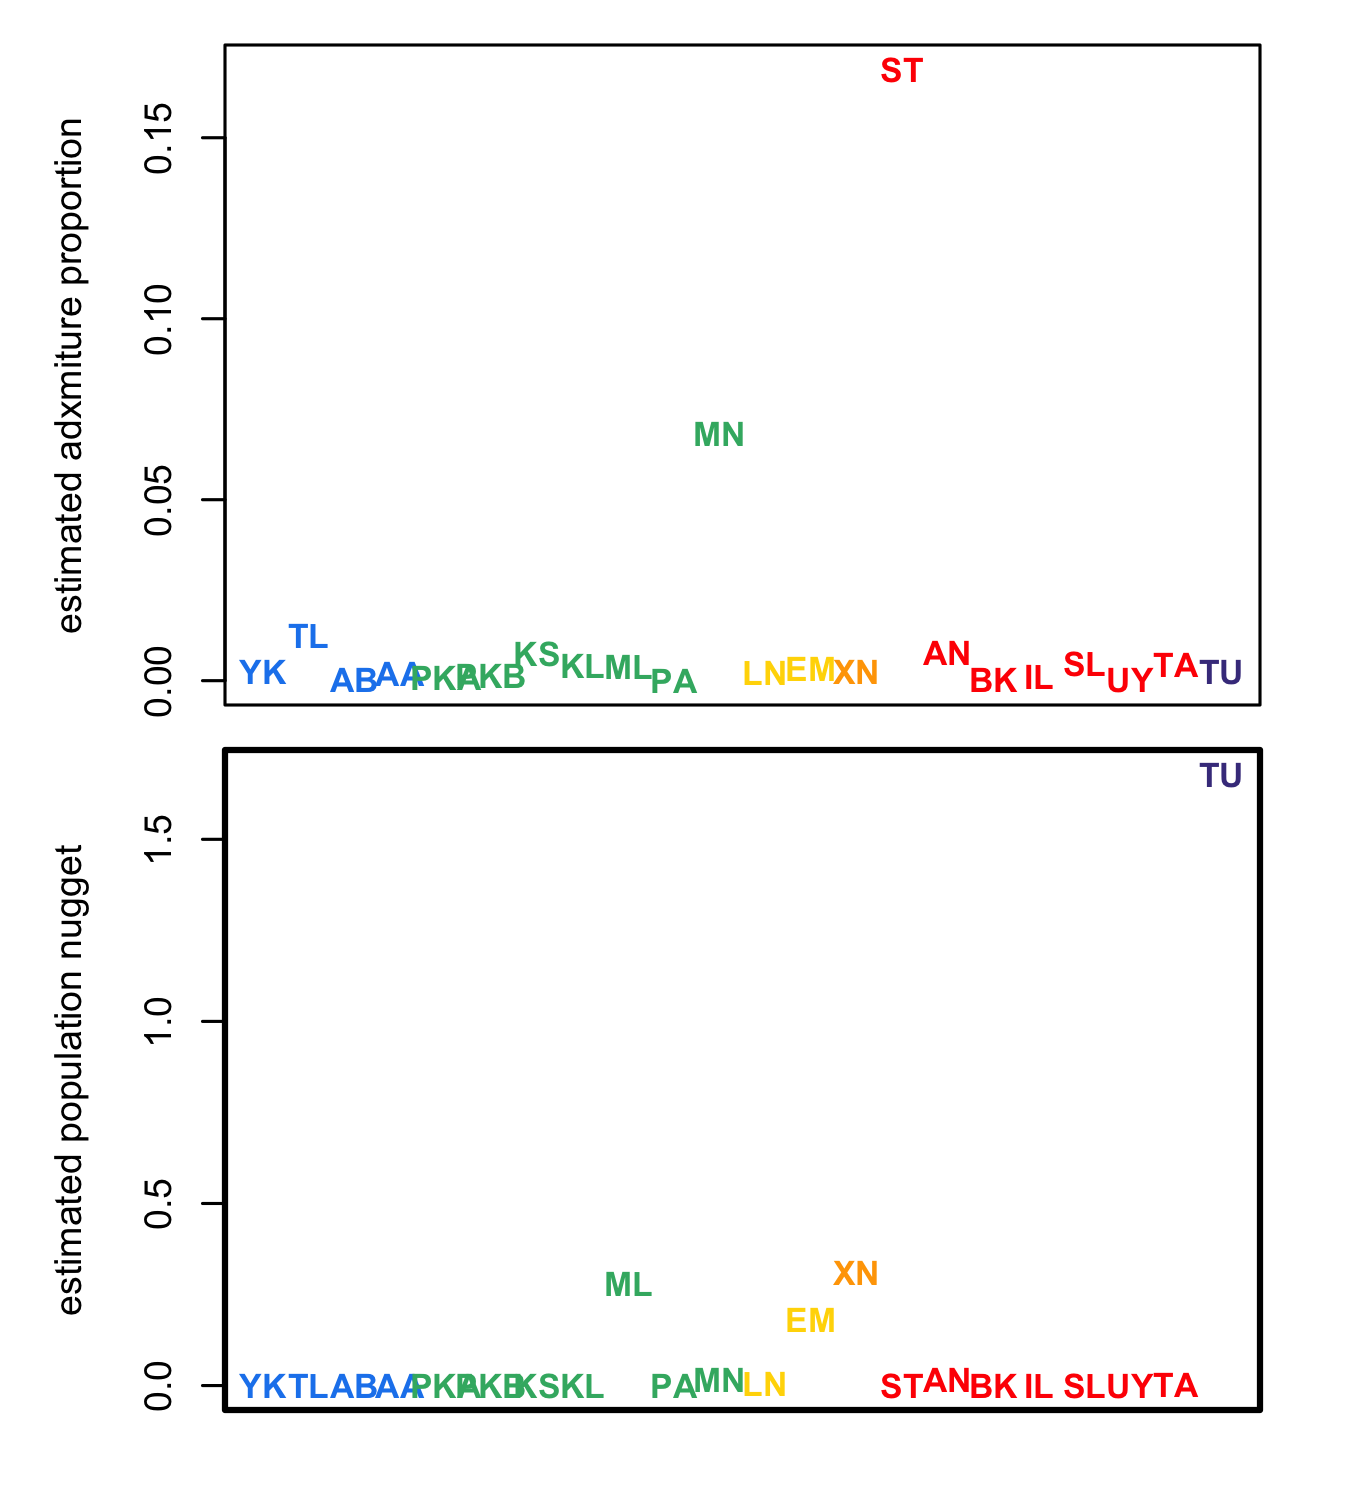
\includegraphics[width=2.4in,height=2in]{figs/warblers/population_warbler_admix_values_nugget.png}}
		\subcaptionbox{Map inferred using SpaceMix \label{warb_pop_no_arrows}}
			{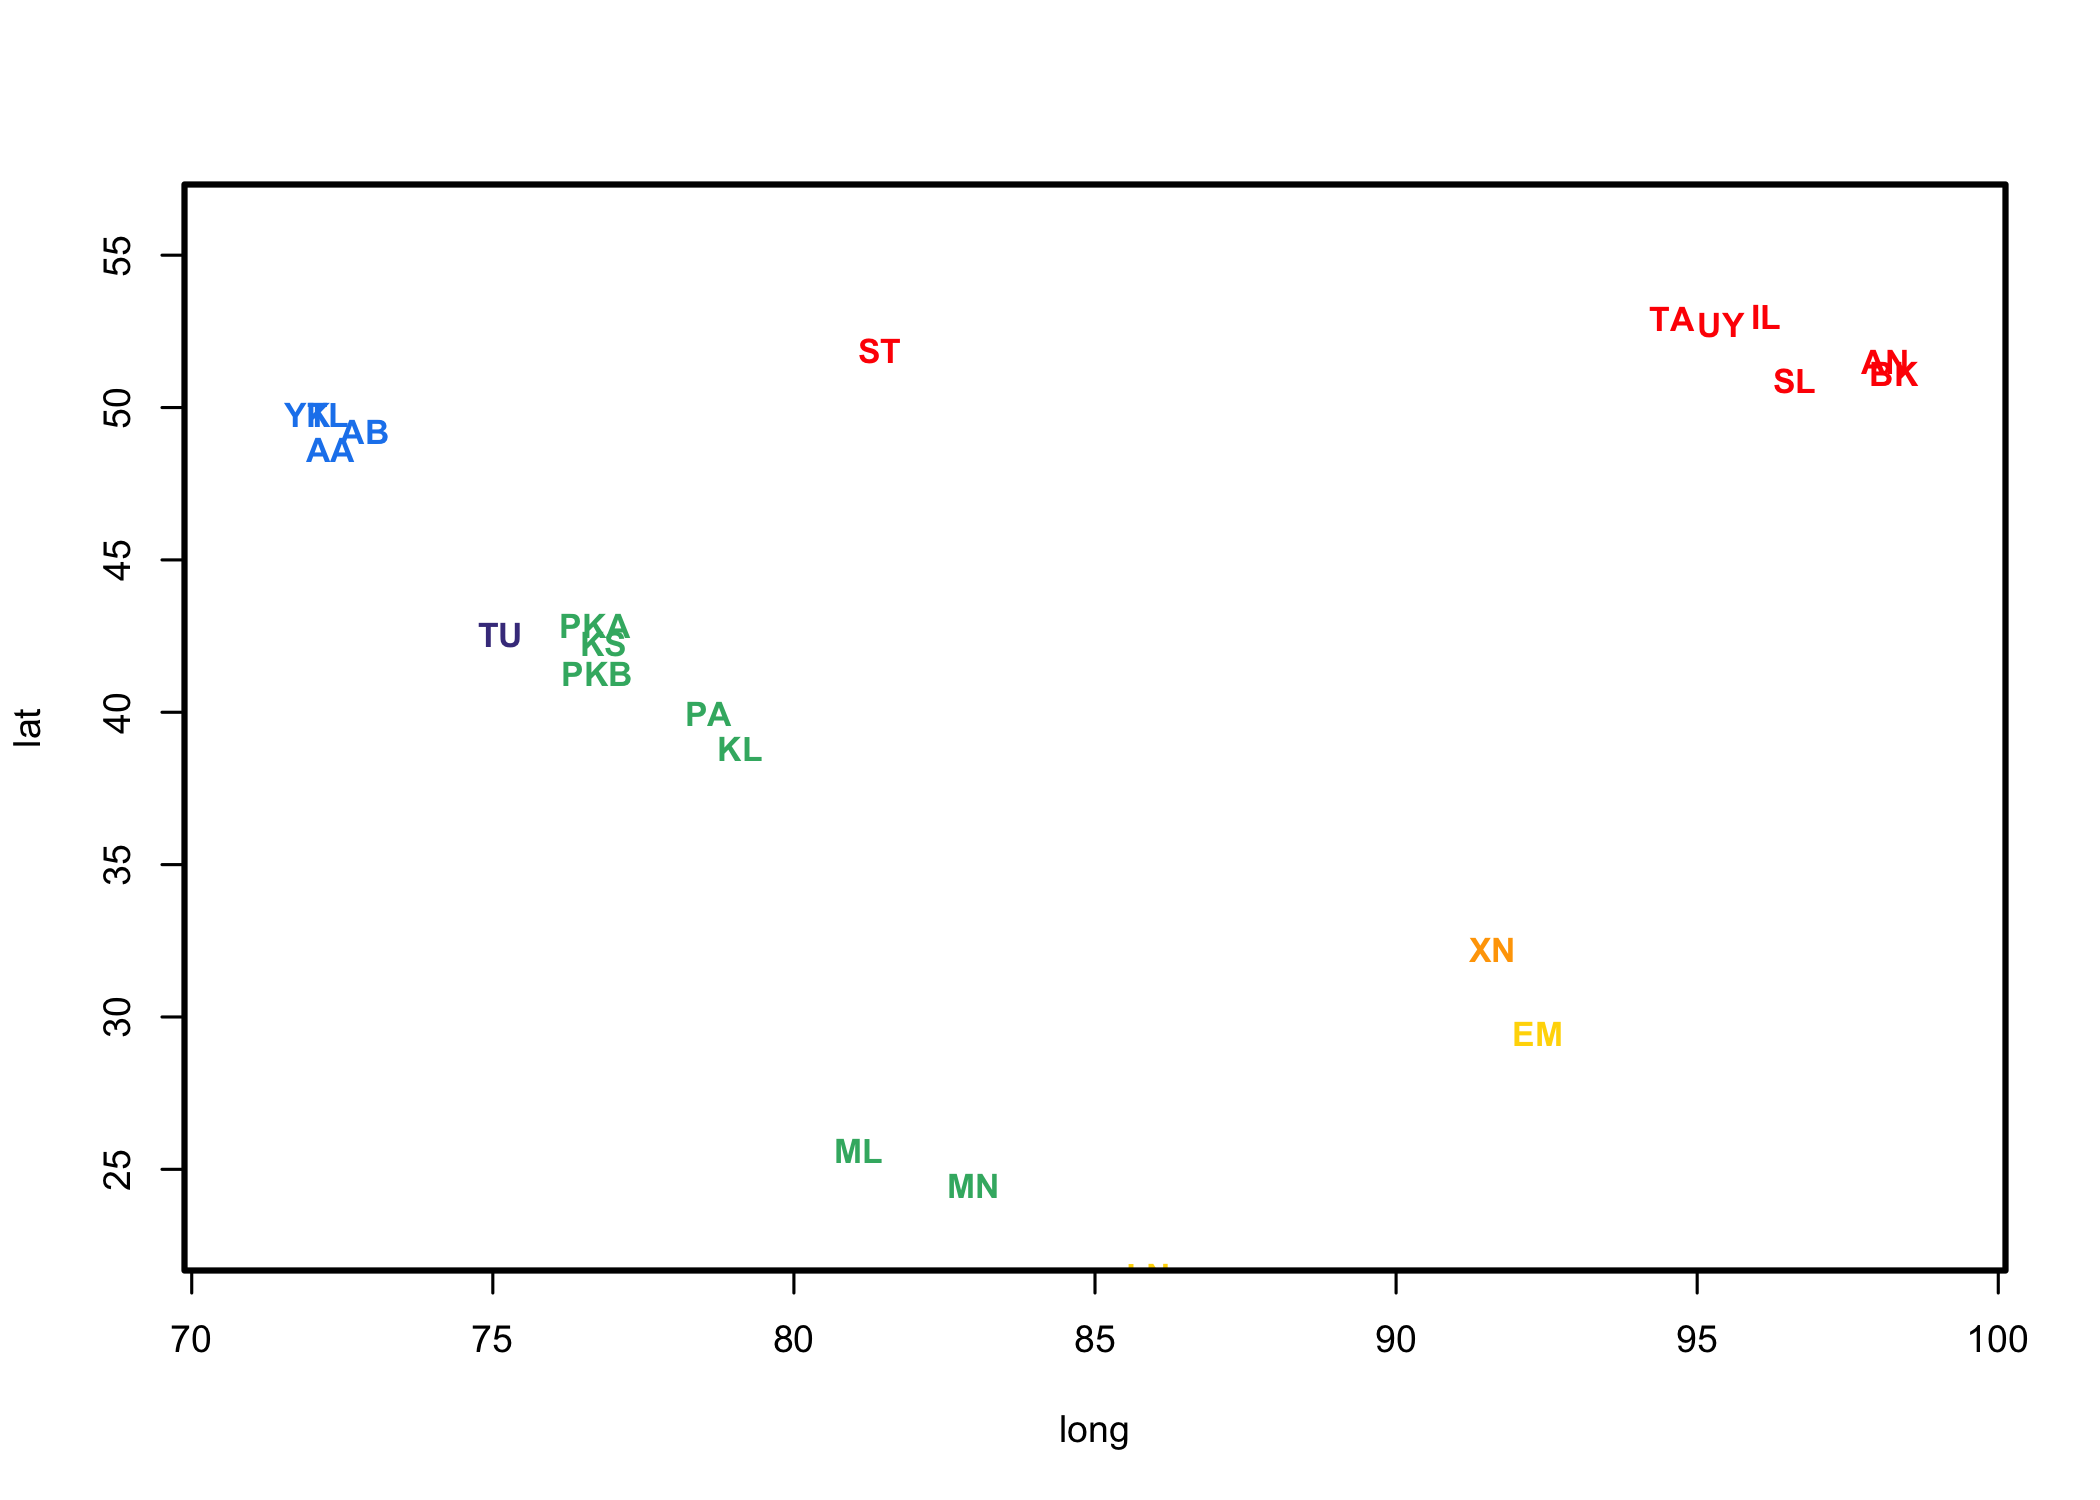
\includegraphics[width=2.4in,height=2in]{figs/warblers/population_warbler_map_no_arrows.png}}
		\subcaptionbox{Map inferred using SpaceMix with admixture arrows shown \label{warb_pop_arrows}}
			{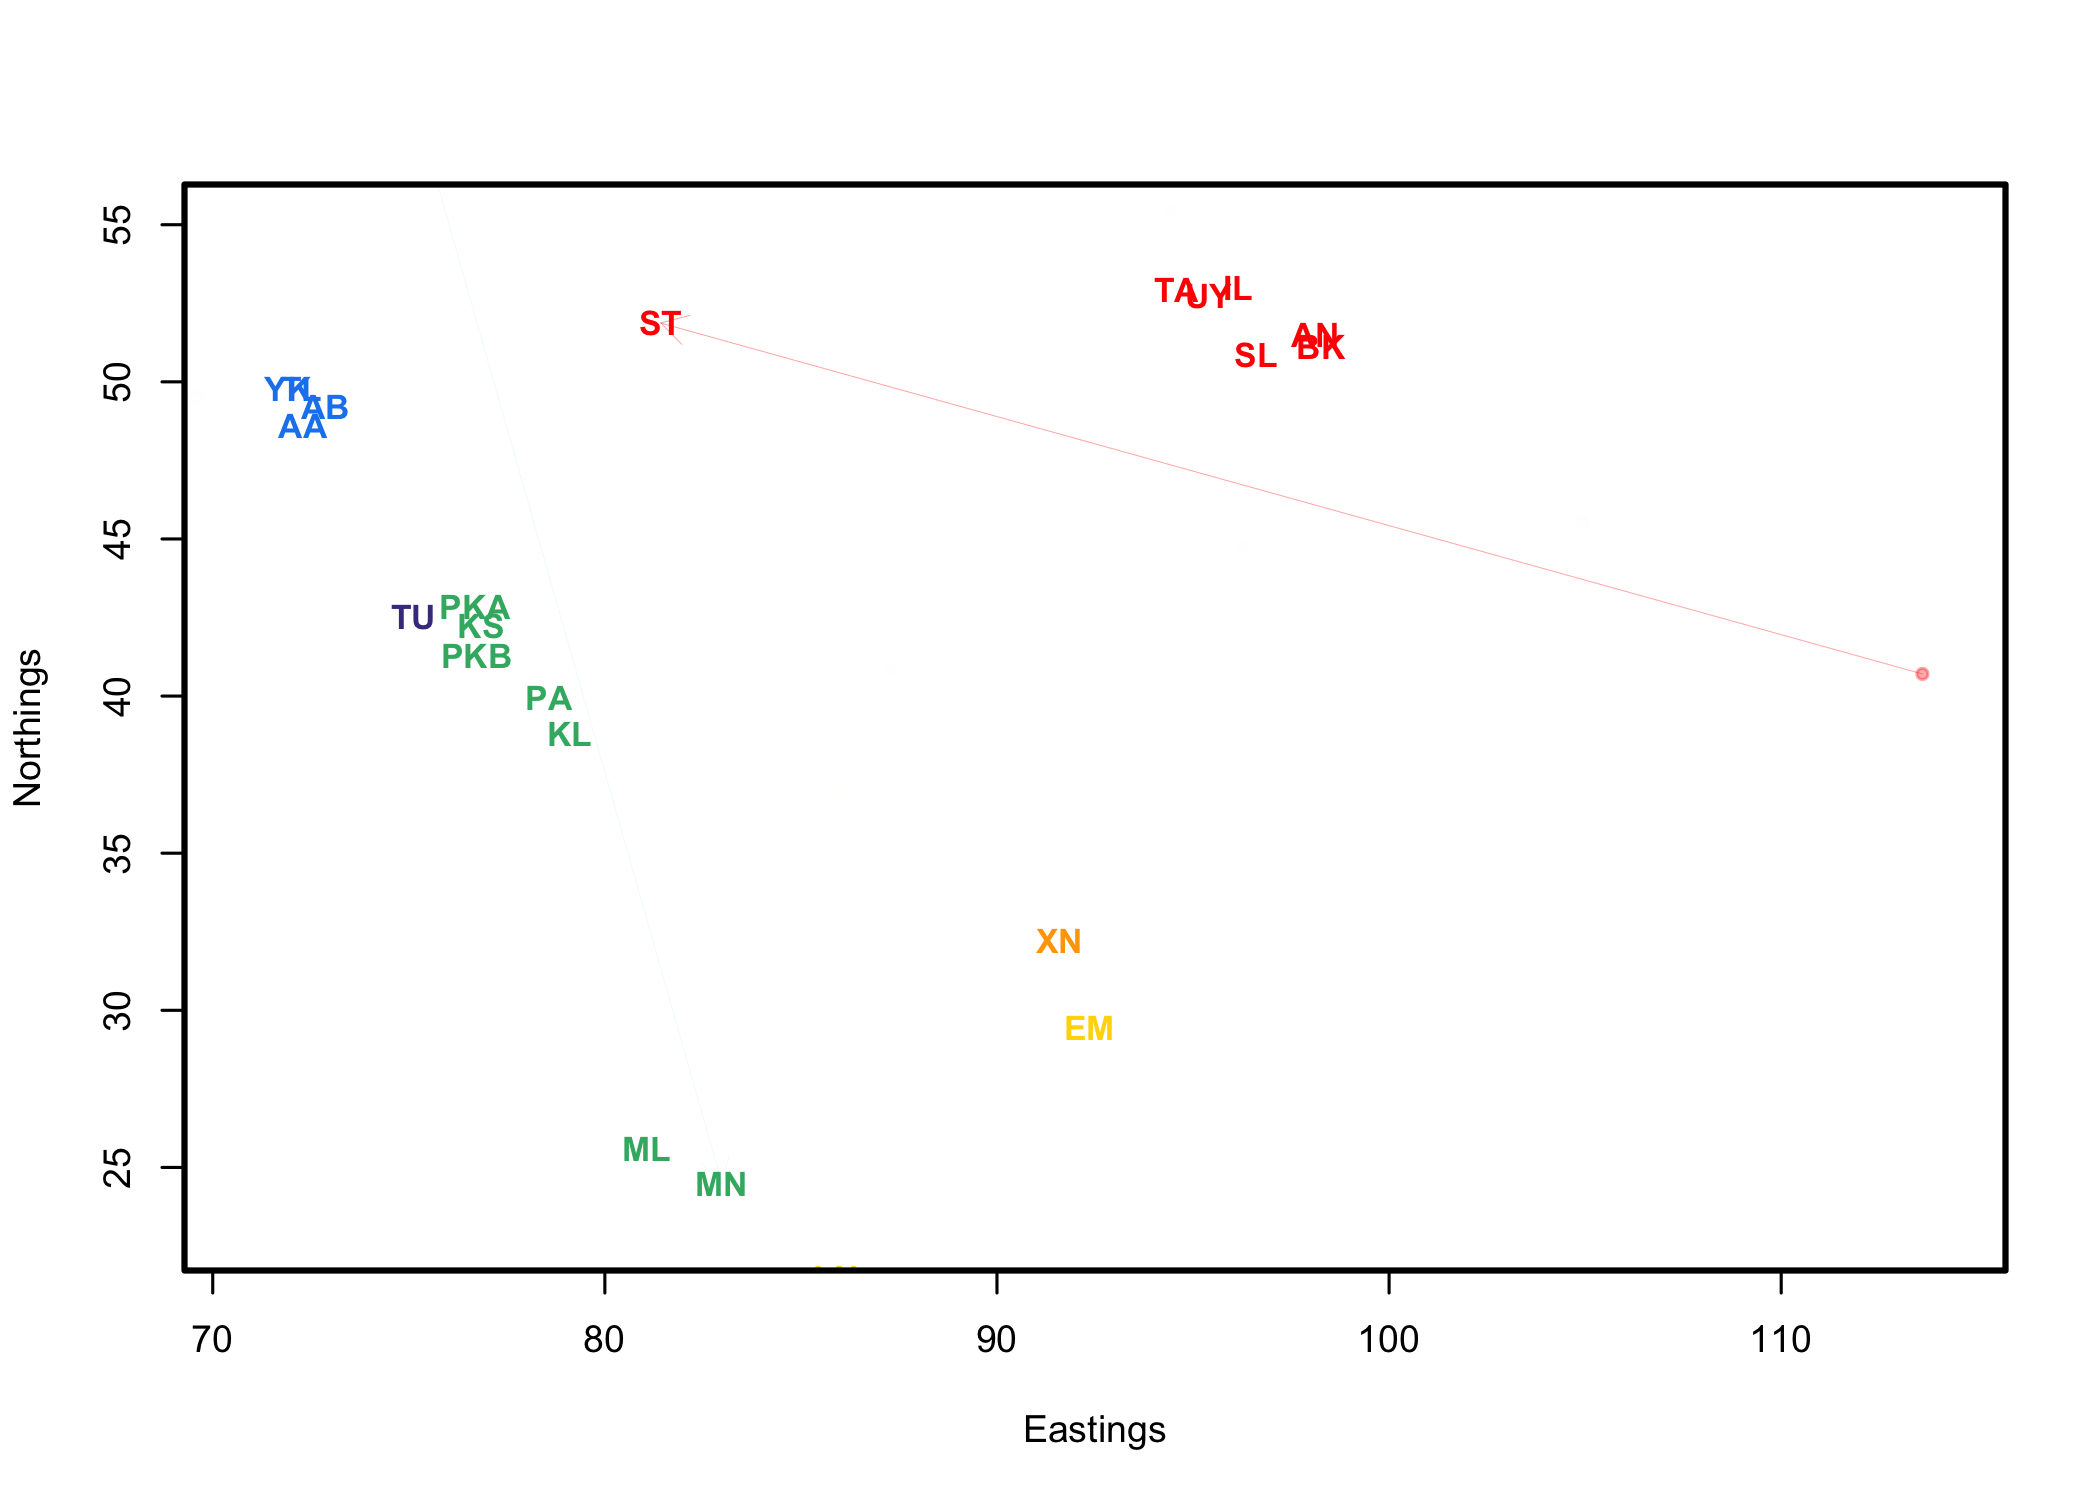
\includegraphics[width=2.4in,height=2in]{figs/warblers/population_warbler_map_randpr1.png}}
	\caption{Greenish warbler subspecies distributions contrasted with maps of all 22 sampled populations inferred using SpaceMix.  For clarity of presentation, the inferred coordinates and parameter values are taken from the single draw of the MCMC with the highest posterior probability and have have been Procrustes transformed around the coordinates of the lattice used to simulate the data. (a) Greenish warbler subspecies distribution map (from Irwin et al NNN).  (b) Inferred population admixture proportions and nugget parameters. (c) Inferred population map without admixture arrows shown, with population labels colored as in (a). (d) Inferred population map with admixture arrows (with thickness proportional to inferred admixture proportion) shown, with population labels colored as in (a). }\label{sfig:warbler_pops}
\end{figure}

\gc{run method w. no admixture. I think we should define the random priors in the methods above, as it's not specific to any of the analyses}

\gc{We first ran spacemix on the population dataset, with no admixture, setting the prior locations of the populations at random (as described above).} The inferred map (Figure \ref{sfig:warbler_pops}) largely recapitulates the geography of the sampled populations.  Populations choose locations around a large ring, with ordering similar to that of their true geographic locations.  The Turkish population (\textit{Phylloscopus trochiloides} ssp. \textit{nitidus}) clustered with the populations in the subspecies \textit{ludlowi}, but also chose a relatively high nugget parameter, reflecting the independent drift it does not share with its \textit{ludlowi} neighbors.  The Yekat population of \textit{viridanus} individuals clusters closely with the other, less far-flung \textit{viridanus} individuals, indicating that differentiation within that subspecies is not commensurate with the amount of IBD expected for samples separated by that much distance. 

In the north, where the twin waves of expansion around the Tibetan Plateau are hypothesized to meet, the inferred \gc{geogenetic} distance between populations identified as \textit{Phylloscopus trochiloides} ssp. \textit{plumbeitarsus} and ssp. \textit{viridanus} was \gc{much} greater than their observed geographic separation, reflecting the reproductive isolation between these adjacent forms \gc{{\bf POINT to graph showing this in supp}.  Interestingly, the ST population, which consists of six individuals sampled in Stolby, Russia, chooses a location intermediate between the \textit{plumbeitarsus} and \textit{viridanus} groups. The Stolby sample is composed of three individuals that belong to the eastern \textit{plumbeitarsus} and three individuals that belong to the western \textit{viridanus} \cite{Alcaide et al (2014)}. In the case where no admixture is allowed this population is forced to adopt an intermediate position to incorporate its admixed nature. }

%However, where the population-level analysis shows the Stolby population intermediate between the \textit{viridanus} and \textit{plumbeitarsus} clusters, the individual-level analysis reveals that the Stolby population (n=6)

We then ran the method allowing admixture, and again discuss the random priors results. The Stolby population chooses the highest admixture proportion, with a mean of 0.19 \textbf{95\% credible intervals}.  Multiple runs agreed well on the level of admixture of the Stolby (see caption of Supplementary Figure \ref{sfig:warbler_pop_compare}). What does vary across runs, is whether the Stolby population chooses to locate itself by the \textit{viridanus} cluster and draw admixture from near the \textit{plumbeitarsus}  cluster or vise versa, however, this is to be expected given the 50/50 nature of the sample (Supplementary Figure \ref{sfig:warbler_pop_compare}). 

%\gc{Graham: dont feel like we need the three analyses in main text.} Across the three independent analyses (two with the observed population locations as spatial priors on the locations, $G'$, that they choose for themselves, one with random locations as spatial priors), the inferred values of admixture proportion are consistent (95\% credible intervals:  0.146-0.233, 0.154-0.242, 0.146-0.238).  However, both the position that the Stolby population chooses for itself and the region from which it draws admixture varies between runs (Figure \ref{sfig:warbler_pop_compare}).  In two of the analyses, the Stolby population moves to a position proximate to the \textit{viridanus} cluster and chooses admixture from a point beyond the \textit{plumbeitarsus} cluster, and in one analysis, this pattern is reversed.  

\begin{figure}
	\centering
		\subcaptionbox{\label{warb_pop_realpr1}}
			{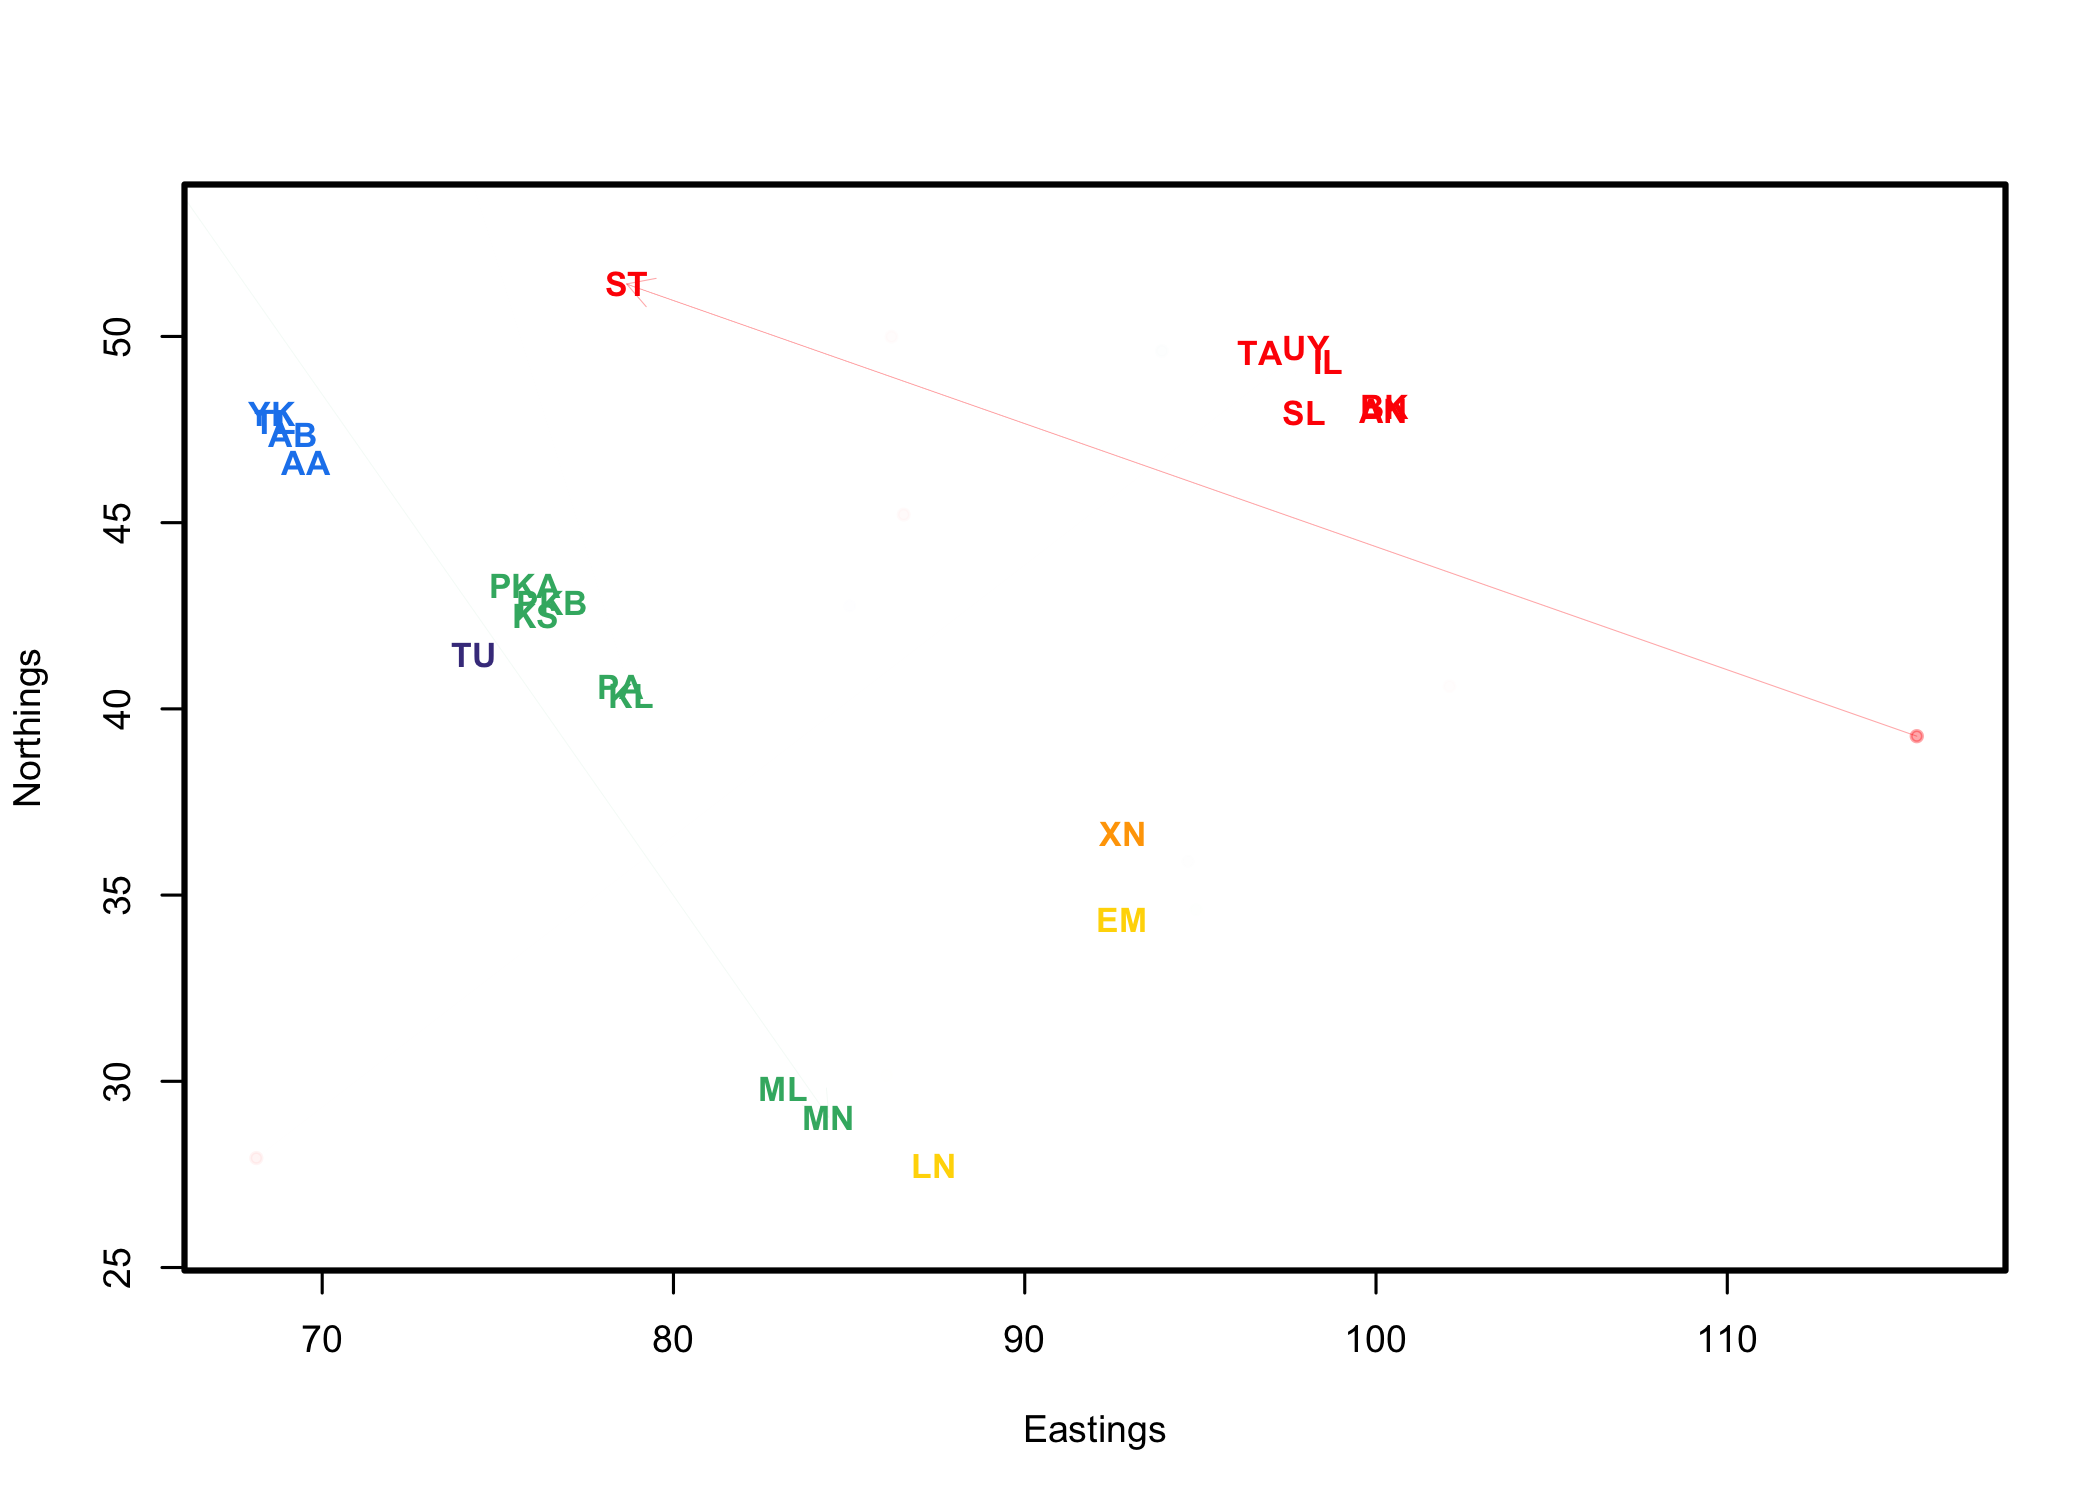
\includegraphics[width=1.85in,height=1.54in]{figs/warblers/population_warbler_map_realpr1.png}}
		\subcaptionbox{\label{warb_pop_realpr2}}			
			{\includegraphics[width=1.85in,height=1.54in]{figs/warblers/population_warbler_map_realpr2.png}}
		\subcaptionbox{\label{warb_pop_randpr1}}
			{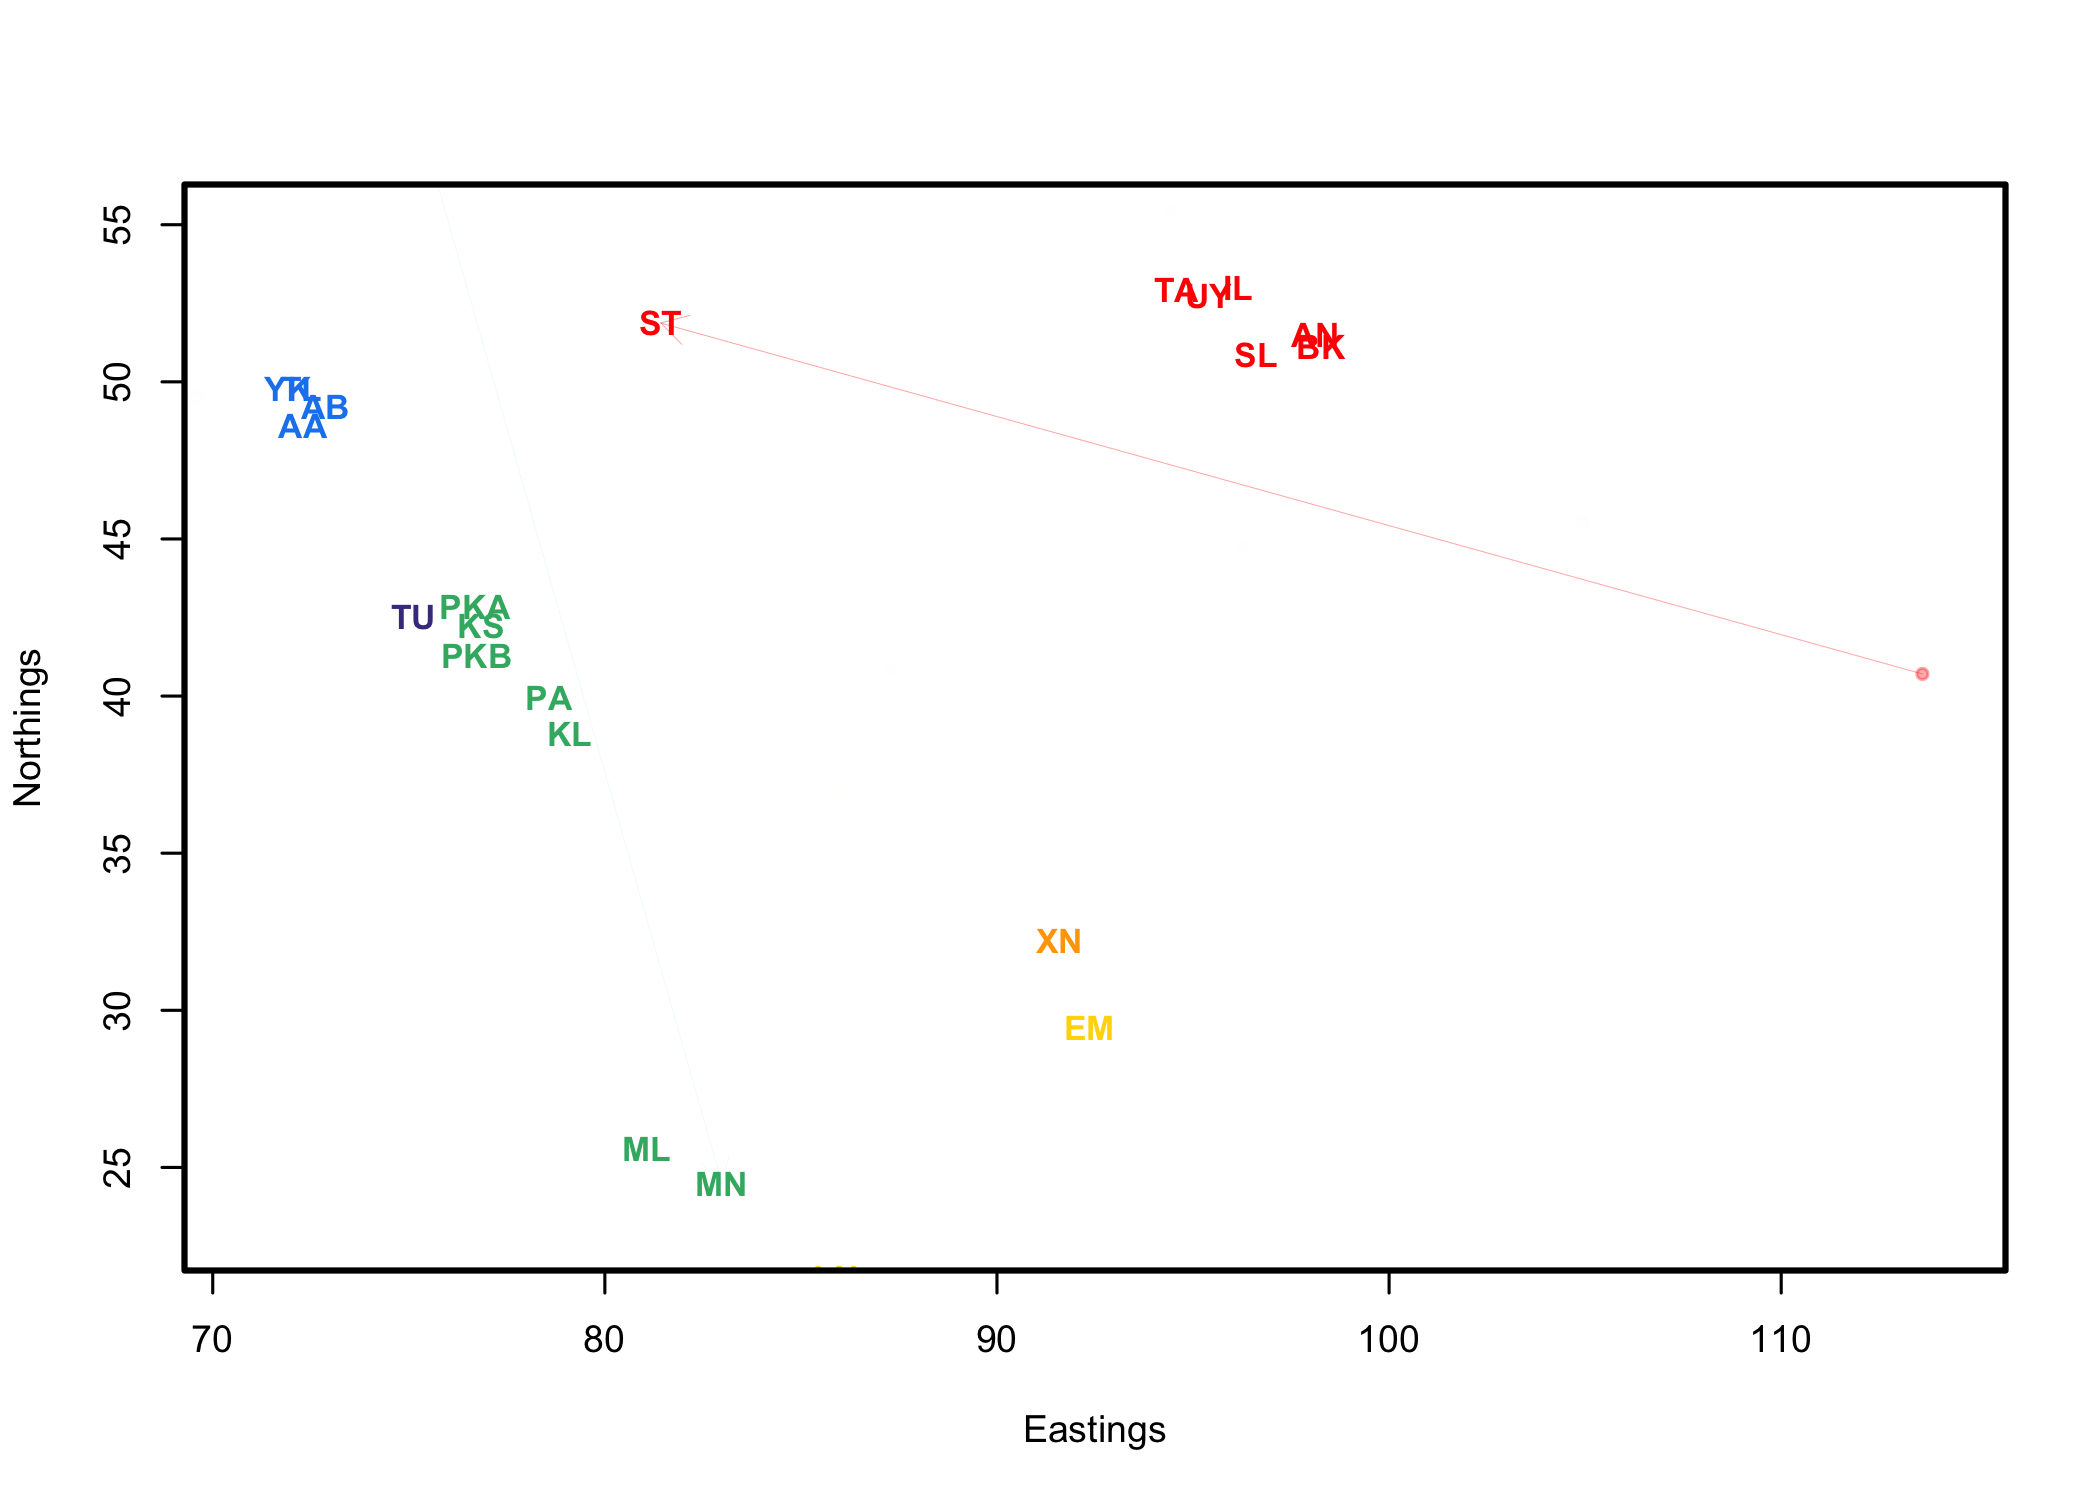
\includegraphics[width=1.85in,height=1.54in]{figs/warblers/population_warbler_map_randpr1.png}}
	\caption{Comparison of inferred maps from three independent analyses.  (a,b) Results from analysis using observed locations as priors on population locations.  (c) Results from analysis using random, uniformly distributed locations within the observed range of latitude and longitude as priors on population locations.}\label{sfig:warbler_pop_compare}
\end{figure}

Because \textit{a priori} assigned population membership may be artificial (individuals from more than one population may be sampled at a single site), we repeated these analyses on an individual level.  In these analyses, the sample size in each `population' was 2 (for the two alleles in a diploid), and each individual chose its own location as well as the location of its source of admixture, the proportion of that admixture, and its nugget.  As with the analysis on multi-sample populations, the results \gc{approximately} mirror the geography of the individuals.  \gc{Individuals choose very low levels of admixture...}

%The order of individuals' estimated locations around the Plateau is largely concordant with their true locations, and, in most cases, individuals sampled from the same population cluster closely together, as would be expected if samples collected at a single site are draws from a population that is locally panmictic.  

\begin{figure}
	\centering
		\subcaptionbox{Inferred map of warbler individuals \label{warb_ind_map}}
			{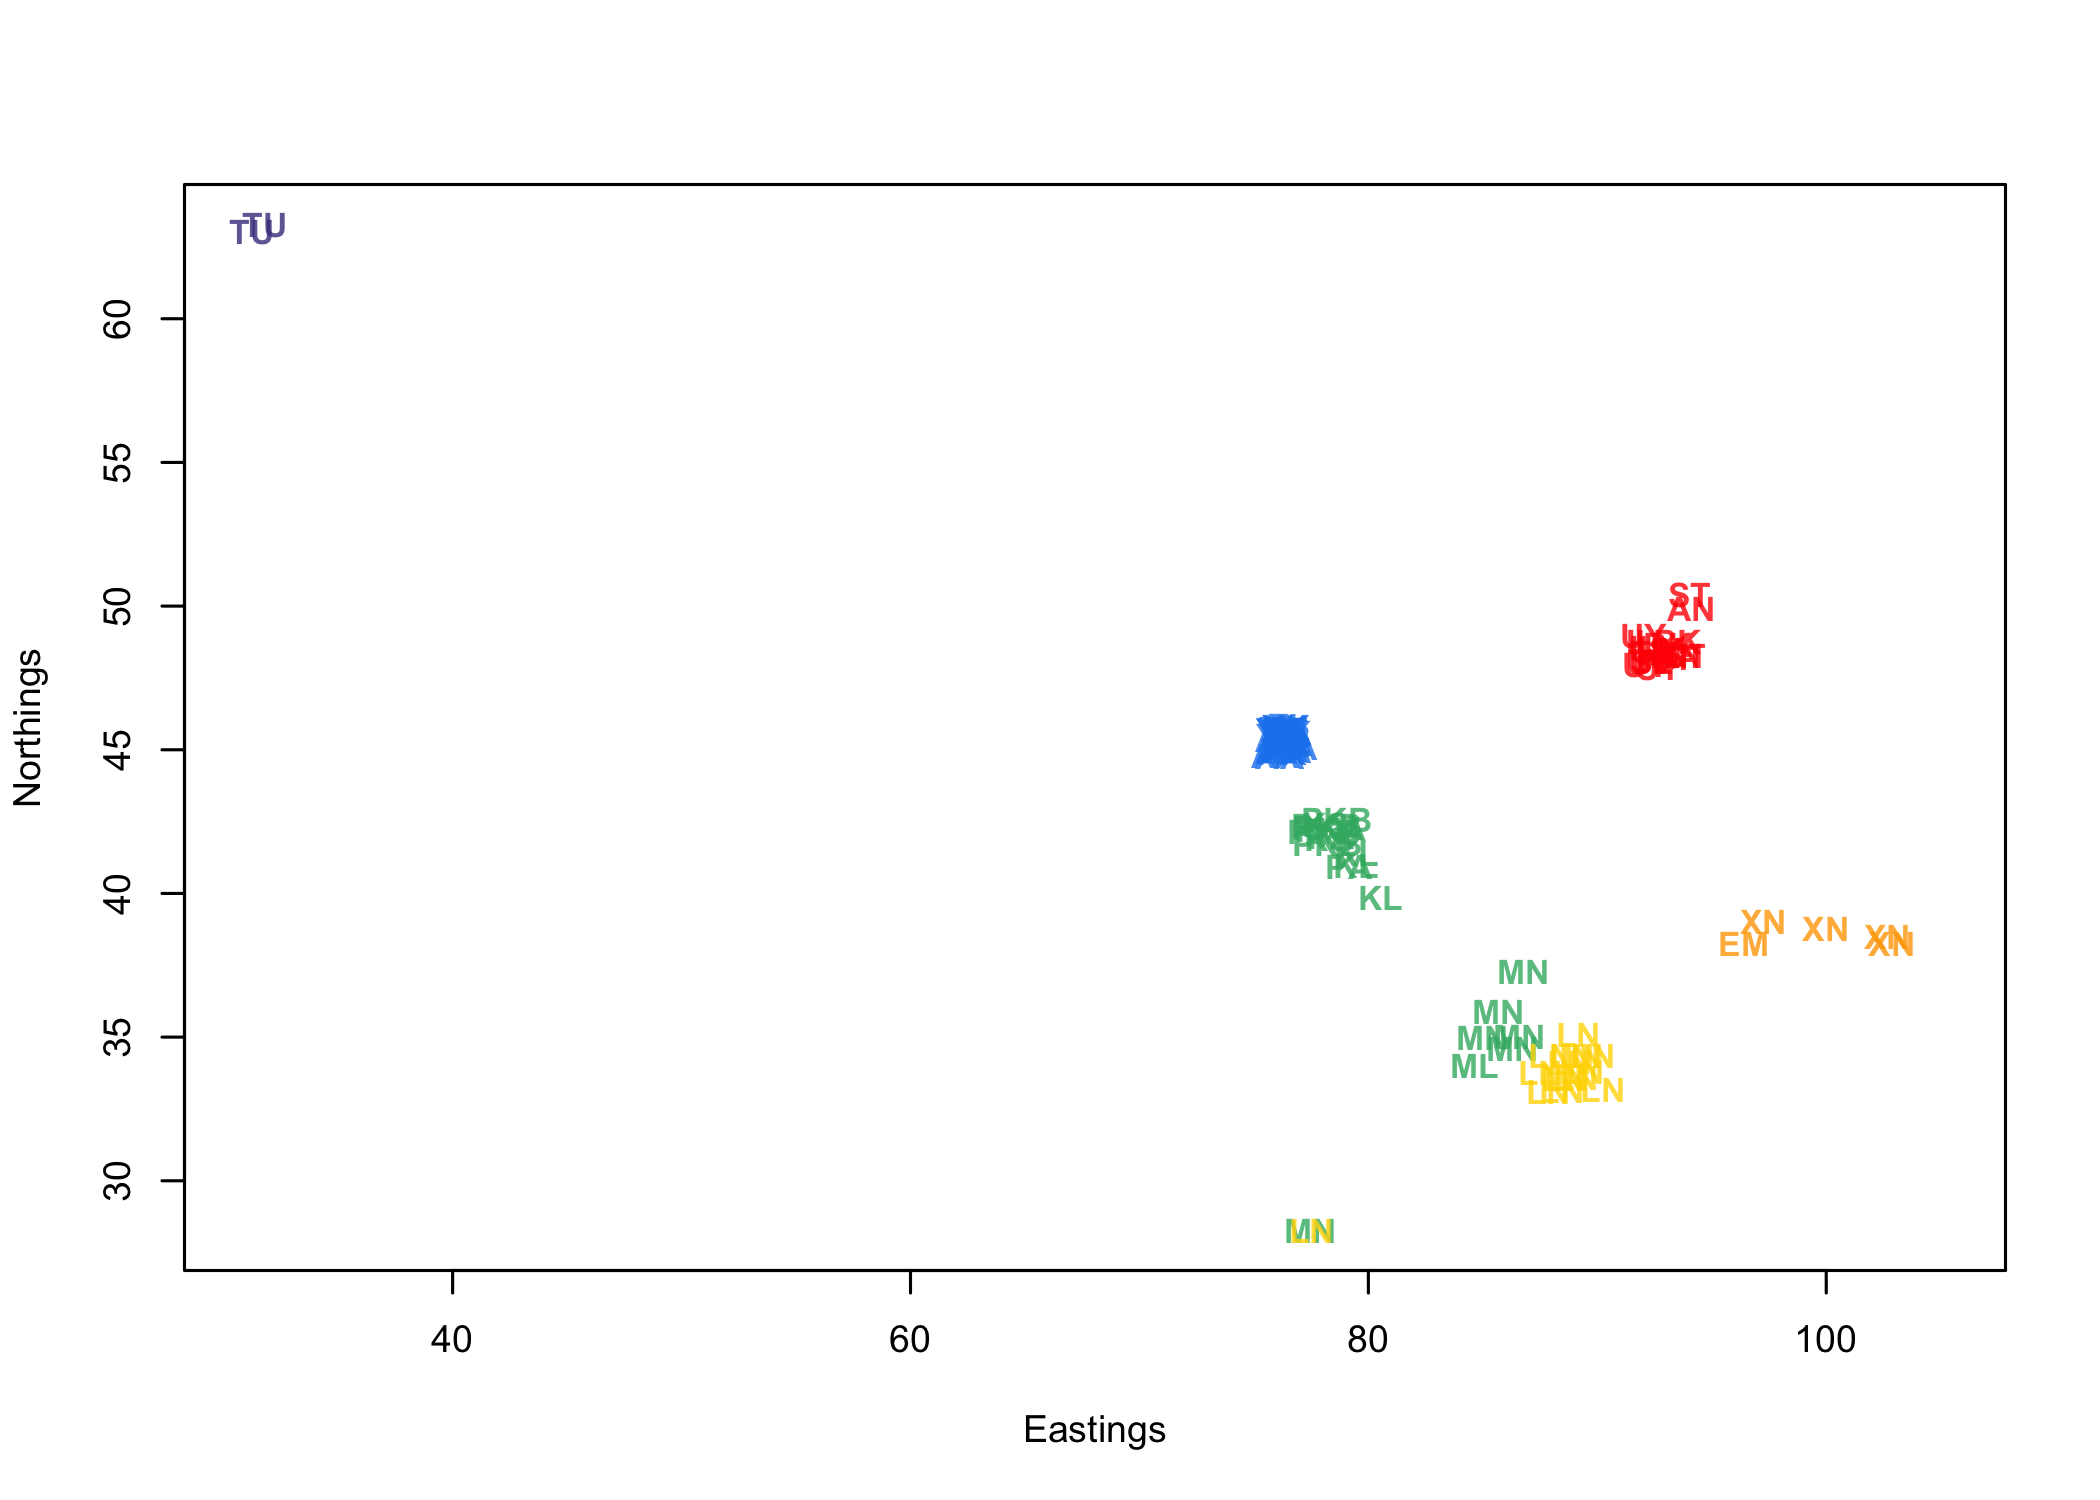
\includegraphics[width=2.8in,height=2.3in]{figs/warblers/individual_warbler_map_noarrows_randpr1.png}}
		\subcaptionbox{Closeup of non-\textit{nitidus} samples \label{warb_ind_map_closeup}}
			{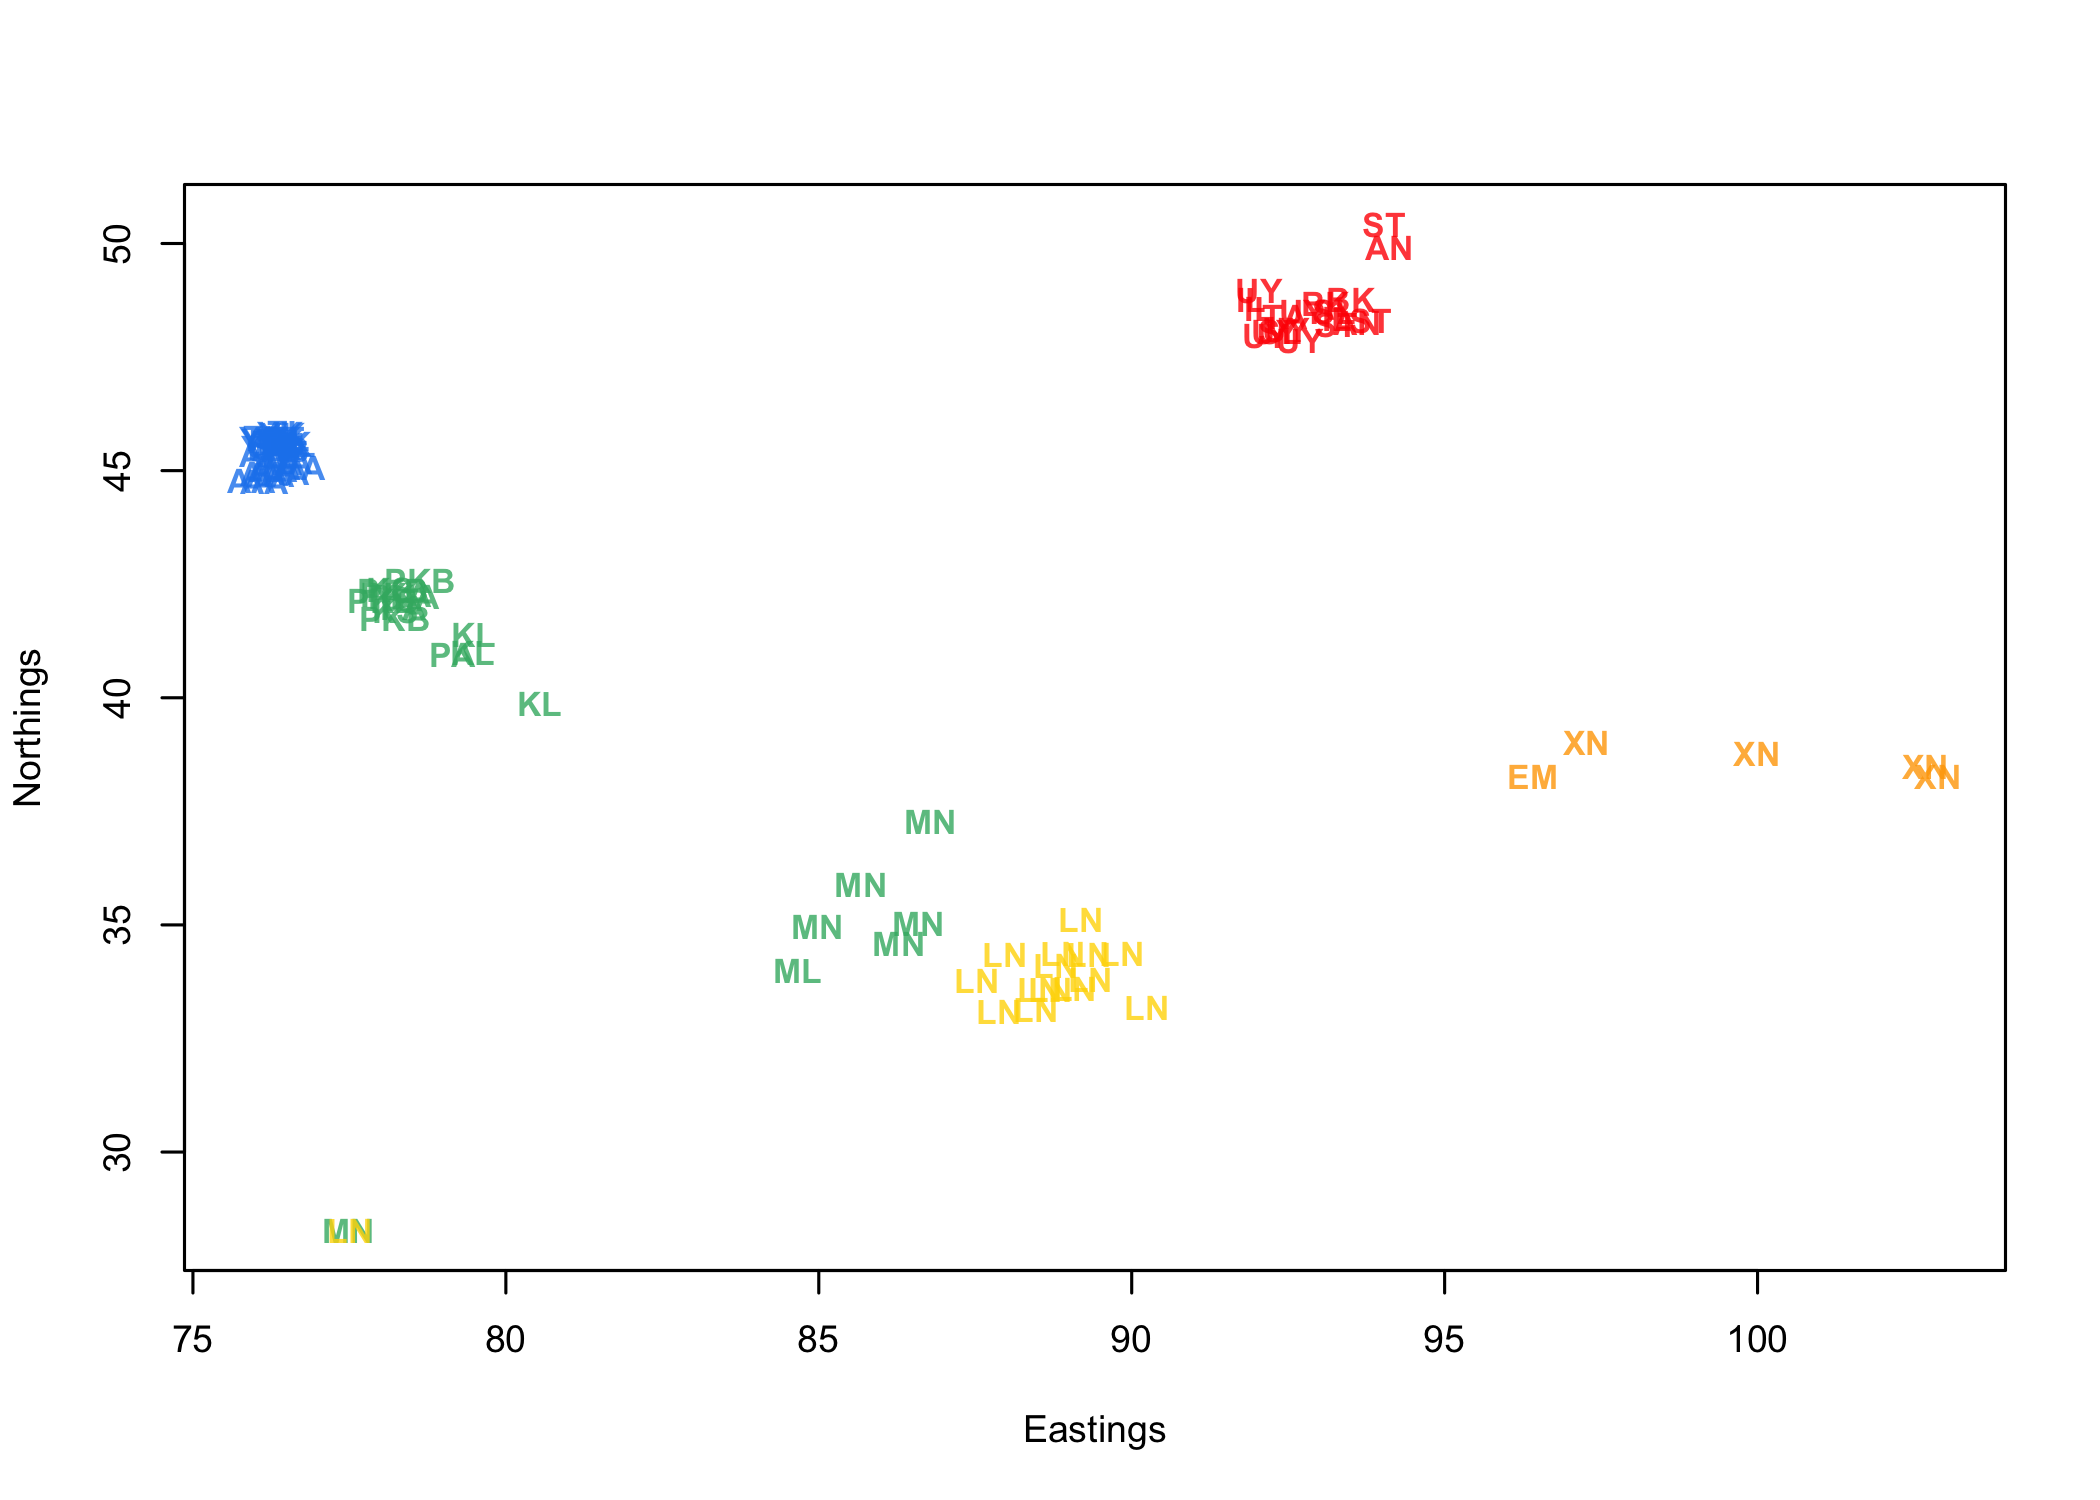
\includegraphics[width=2.8in,height=2.3in]{figs/warblers/individual_warbler_map_noarrows_closeup_randpr1.png}}
	\caption{Inferred maps for individual warbler individuals, colored by subspecies. (a) complete map including Turkish \textit{nitidus} samples.  (b) close up of all non-\textit{nitidus} samples.}\label{sfig:warbler_inds}
\end{figure}

There are a number of obvious departures in the individual inferred geogenetic map from the observed map. The most obvious again is the clear split between \textit{viridanus} and \textit{plumbeitarsus} individuals in the north at the contact zone of the two waves of expansion.  This is clearer now than in the population-based analysis as individuals from the Stolby population have moved to near their respective \textit{viridanus} \textit{plumbeitarsus}  clusters. 

Despite the fact that \textit{viridanus} and \textit{plumbeitarsus} individuals have moved away from each other in our geogenetic map, they are still closer to each other than we might expect if their drift is truely independent (e.g. our populations could form along a line). This horseshoe, with \textit{viridanus} and \textit{plumbeitarsus} at its tips, is steady within and among runs of the MCMC and choice of position priors (see Supplementary clouds NNN). Is this biologically meaningful? A somewhat similar horseshoe shape appears when a principal components (PC) analysis is conducted and individuals are ploted on the first two PCs (Alcaide et al (2014), see our Supp. Figure NNN). However, as discussed by Novembre \& Stephens such patterns in PC analysis can arise for somewhat unintuitive reasons. If populations are simulated under a one dimensional stepping stone model, then plotting individuals on the first two PCs results in a horseshoe (e.g. see Supp. Figure NNN) not because of any particular gene flow connection between the tips but rather because of the othogonality requirement of PCs (see Novembre \& Stephens for more discussion). When spacemix is applied to one dimensional stepping stone data, the placement of samples is consistent with a line. In addition when we run Spacemix on the greenish warbler individuals specifying their location priors to fall along a straight line, with samples located at their approximate postions around the horseshoe, the posterior positons of the populations still curl up to form a horseshoe. The proximity of \textit{viridanus} and \textit{plumbeitarsus}  in geogenetic space may be due to gene flow between the tips of the horseshoe north of the Tibetan Plateau. This conclusion is in agreement with that of Alcaide et al (2014) who observed evidence of hybridization between \textit{viridanus} and \textit{plumbeitarsus} using assignment methods.

A second difference between the observed and inferred maps is a pair of individuals, one identified as \textit{P. t. ludlowi} (Lud-MN3), one as \textit{P. t. trochiloides} (Tro-LN11), that choose locations very close to one another and also away from the other individuals sampled at their locations. Examing pairwise sequence difference shows that these two individuals show unusually recent common ancestry (see SuppMat Figure NNN), and therefore are likely expressing their shared ancestry (drift unshared with other \textit{ludlowi} and \textit{trochiloides} individuals) by choosing locations that are close to each other and far from their respective clusters of individuals that were sampled at the same sites. \gc{move the commented out bit below to the caption of the pairwise seq. plot. }

The SpaceMix map also diverges from the observed map in the distribution of individuals from the subspecies \textit{ludlowi}.  These samples were taken from seven sampling locations along the southwest margin of the Tibetan Plateau, but, in the SpaceMix analysis, partition into two main clusters, one near the \textit{trochiloides} cluster, and one near the \textit{viridanus} cluster.  This break between samples from the same subspecies, which is concordant with the findings of Alcaide et al (2014), makes the \textit{ludlowi} cluster unusual compared to the estimated spatial distributions of the other subspecies (see SuppMat Figure NNN).

\begin{figure}
	\centering
	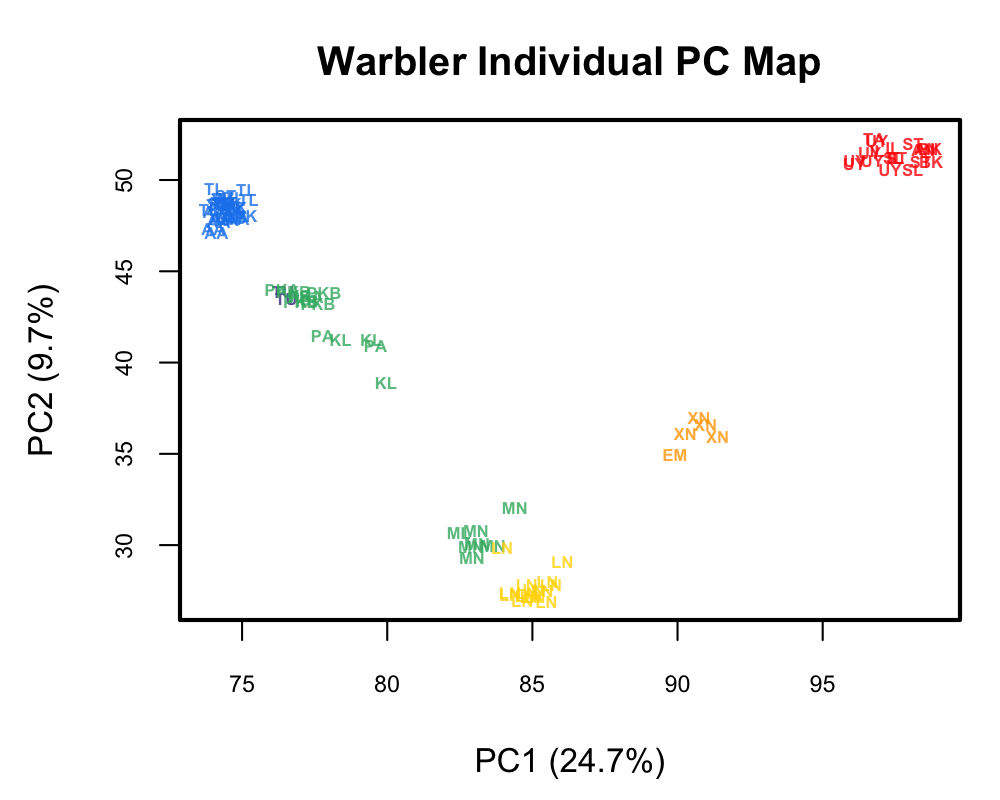
\includegraphics[width=2.4in,height=2in]{figs/warblers/warb_ind_PC_map.png}
	\caption{The map of warbler individuals derived from a Principal Components analysis.}\label{warb_ind_PC_map}
\end{figure}

%
\newpage
\subsection*{Human Populations}
The geography of human population structure is a complex product of the forces of migration, drift, and selection acting on both local and global scales.  Recent work in this area has demonstrated that the signature of these forces can be read in the genomes of modern humans (e.g. Novembre et al 2008, Ralph \& Coop 2013, Moorjani, Reich, ARG folks, Hellenthal et al 2014).  This research has revealed that patterns of spatial genetic differentiation across human populations are byzantine in their complexity, varying across both space (Ralph \& Coop 2013) and time (Skoglund et al 2012, 2014), and shaped by culture (Reich et al 2009, Atzmon et al 2010, Moorjani et al 2011), landscape (Bradburd, Ralph, Coop 2013), and environment (Beall et al 2010, Bigham et al 2010).  To visualize the patterns these processes have induced, we set out to create a geogenetic map for a worldwide sample of modern human populations.  

Specifically, our research questions were: 
\begin{enumerate}
\item What is the geography of human population structure?  Which populations cluster with which, and how does the geogenetic map contrast with the observed geography?
\item Can the map we estimate reconstruct the many of the important expansion events in human pre-history, including the out-of-Africa expansion, the colonizations of Oceania, and the colonization of the Americas via Beringia?
\item Which human populations are most greatly admixed, and from where?  Will the SpaceMix results confirm the admixture findings of previous studies?
\end{enumerate}

\begin{figure}
	\centering
	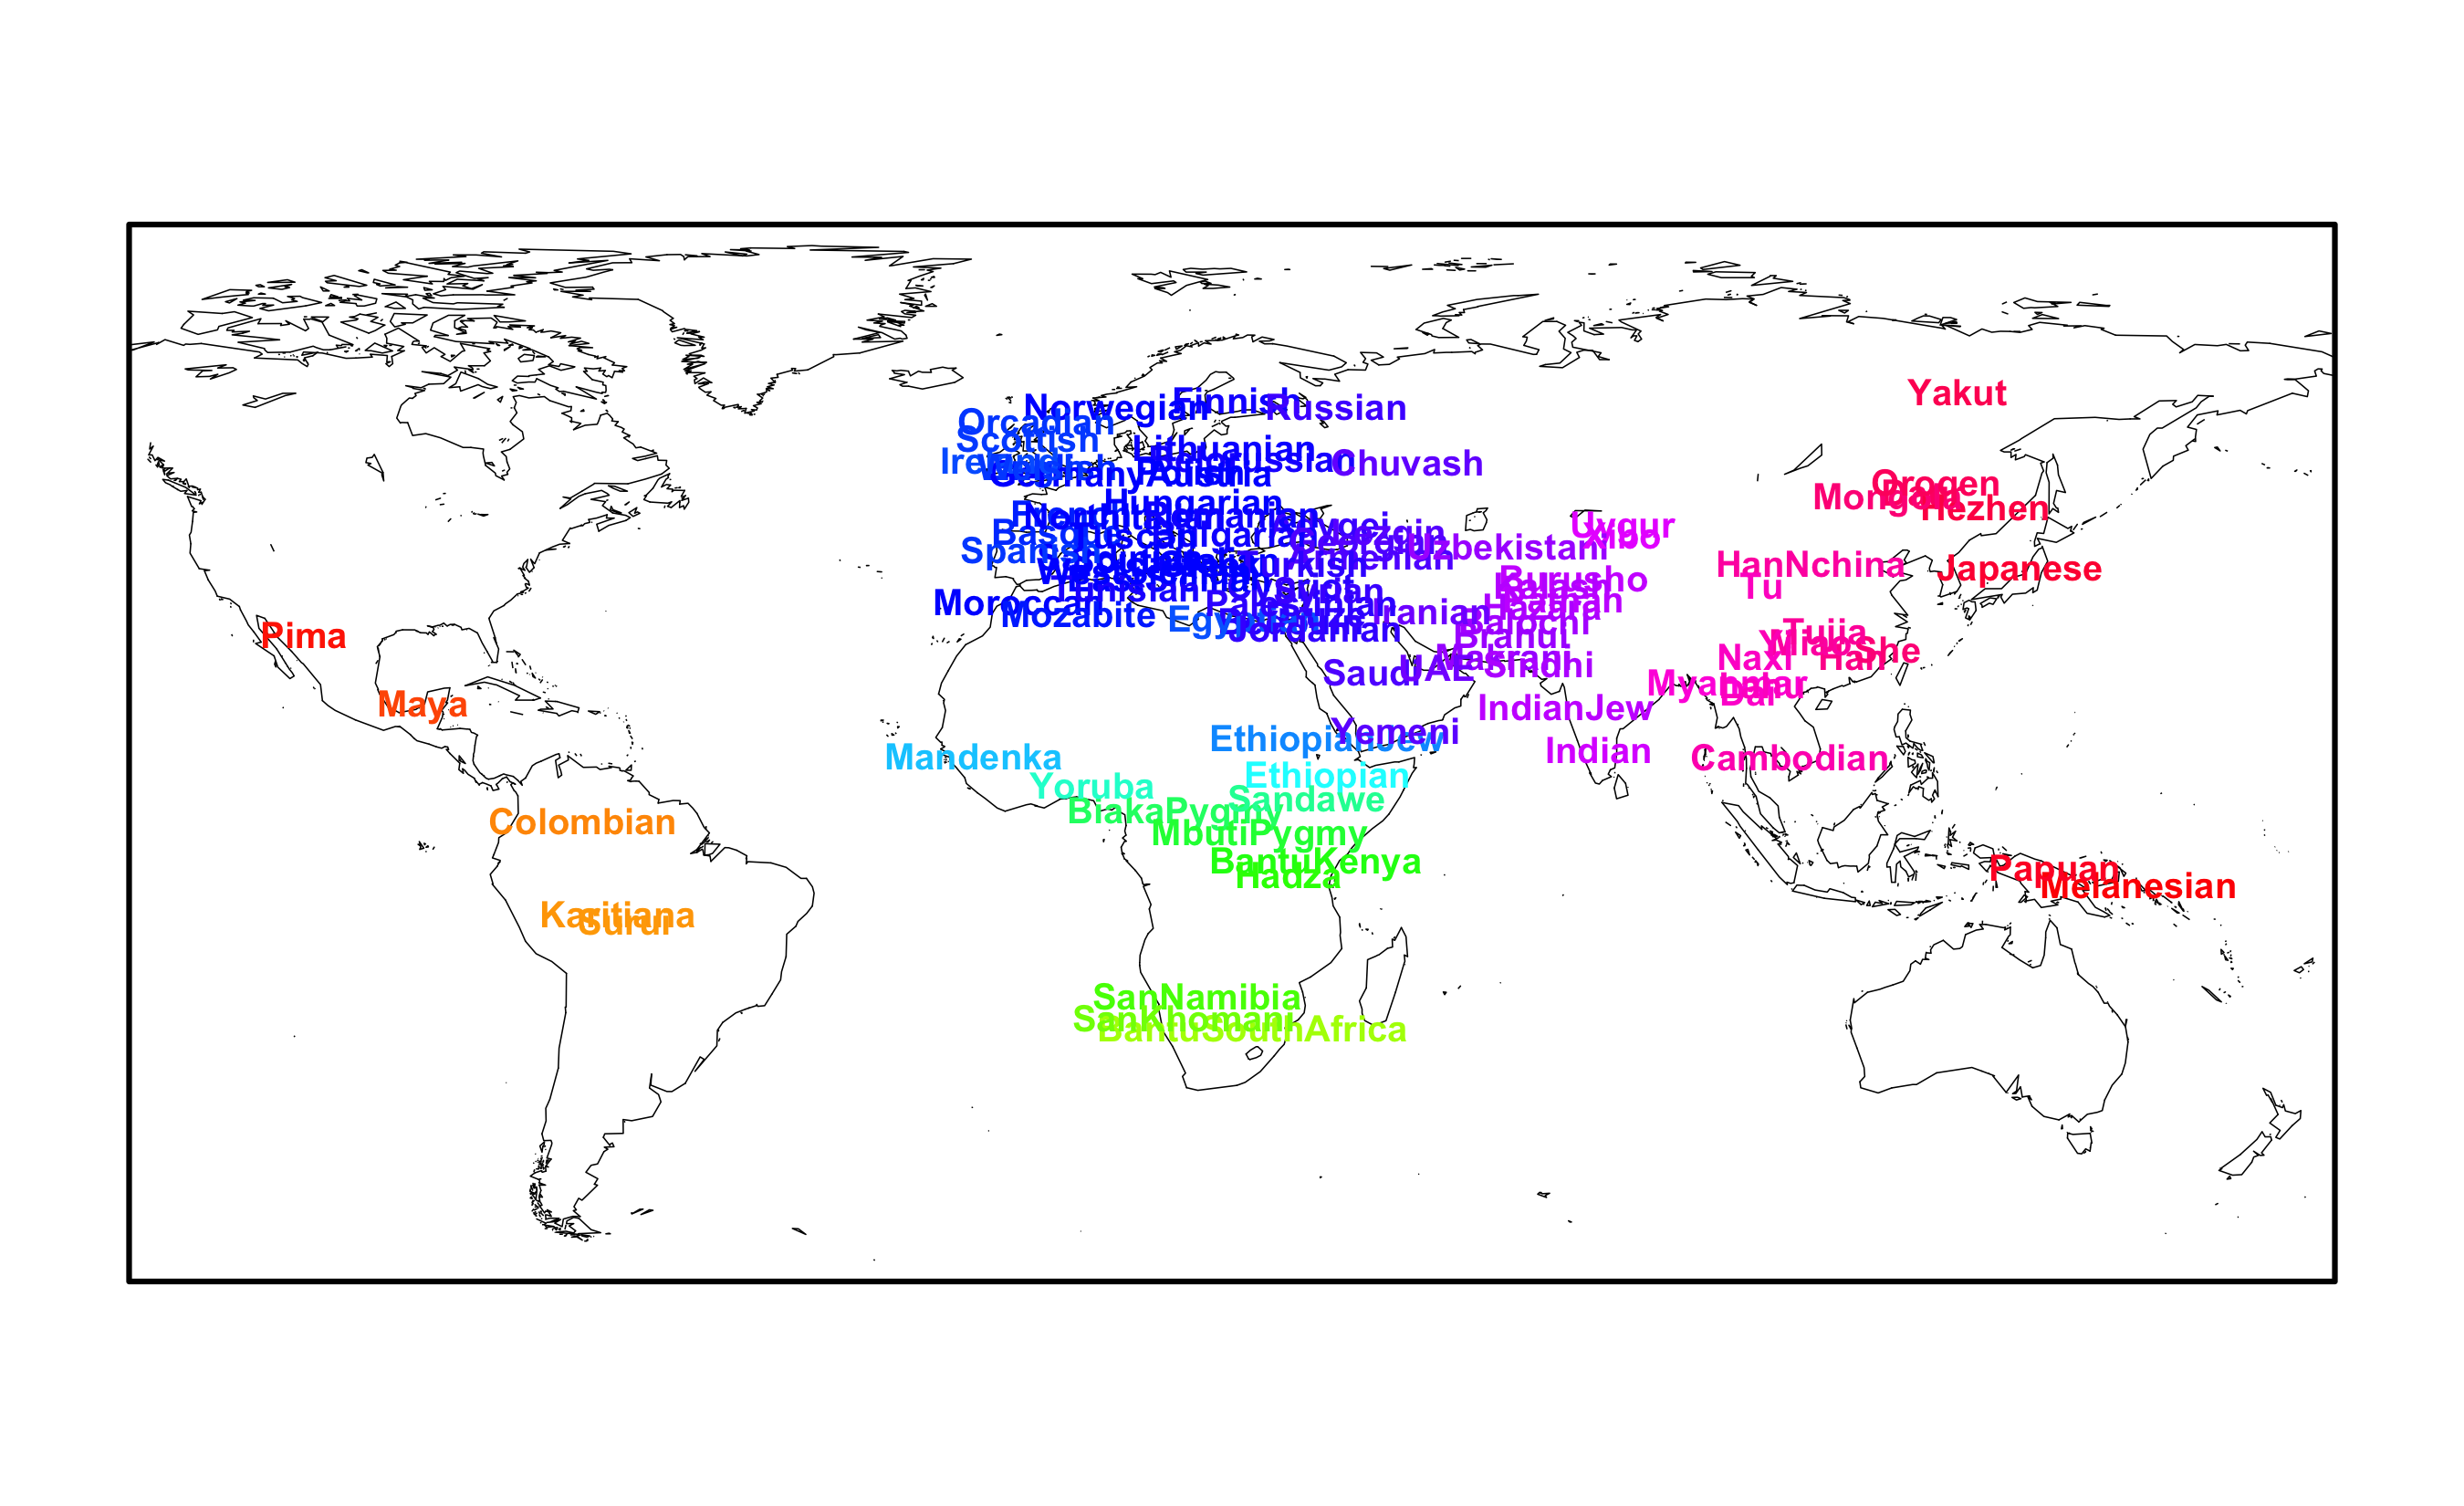
\includegraphics[width=4in,height=2.4in]{figs/globetrotter/globe_world_map_text.png}
	\caption{The map of sampled human populations}\label{globe_world_map}
\end{figure}

\gc{Not totally clear why we are taking 10k SNPs}
To answer these questions, we used a random subset of 10,000 SNPs from the SNP dataset of Hellenthal et al (2014), which is comprised of 1490 sampled in 95 populations (see Fig. \ref{globe_world_map} for map of sampling), as well as the latitude and longitude attributed to each population.  We ran two sets of SpaceMix analyses: in the first, we estimated population locations, and in the second, we estimated population locations, and their admixture sources and amounts.

In the analysis in which populations choose their own locations, the map roughly recapitulates the geography of the samples (Fig. \ref{sfig:globe_noad_maps}).  Populations generally cluster with populations sampled on their continent, and the relative placement of populations is similar to that of their observed geography.  Sub-Saharan African populations are distributed in a manner consistent with their sampled latitude, with the San populations in the south and the Ethiopian populations closest to the Eurasian populations.  North African populations, such as the Moroccan, Tunisian, and Egyptian populations, cluster with Middle Eastern populations such as the Yemeni and the UAE, and are quite close to both the Ethiopian populations and the western European populations, such as the Sicilians, the Cypriots, the Tuscans, and the Sardinians.  Within Eurasia, we see populations grouping roughly in the order of their longitude on the continent, with British, continental European, and Russian populations at the western margin, and Han, Japanese, and Southeast Asian populations such as the Cambodians, the Lahu, and Myanmar on the eastern margin.  Interspersed between are populations of the Sub-continent, such as the Indian, Indian Jewish, and Sindhi populations, as well as populations from farther north in Eurasia that choose intermediate locations between European and East Asian populations, such as the Uygur, the Hazara, the Uzbekistani, and the Chuvash.  Populations from the Americas cluster together and choose a location close to the East Asian populations, as do populations from Oceania.

\begin{figure}
	\centering
		\subcaptionbox{Inferred map of human populations \label{globe_all_noad_map}}
			{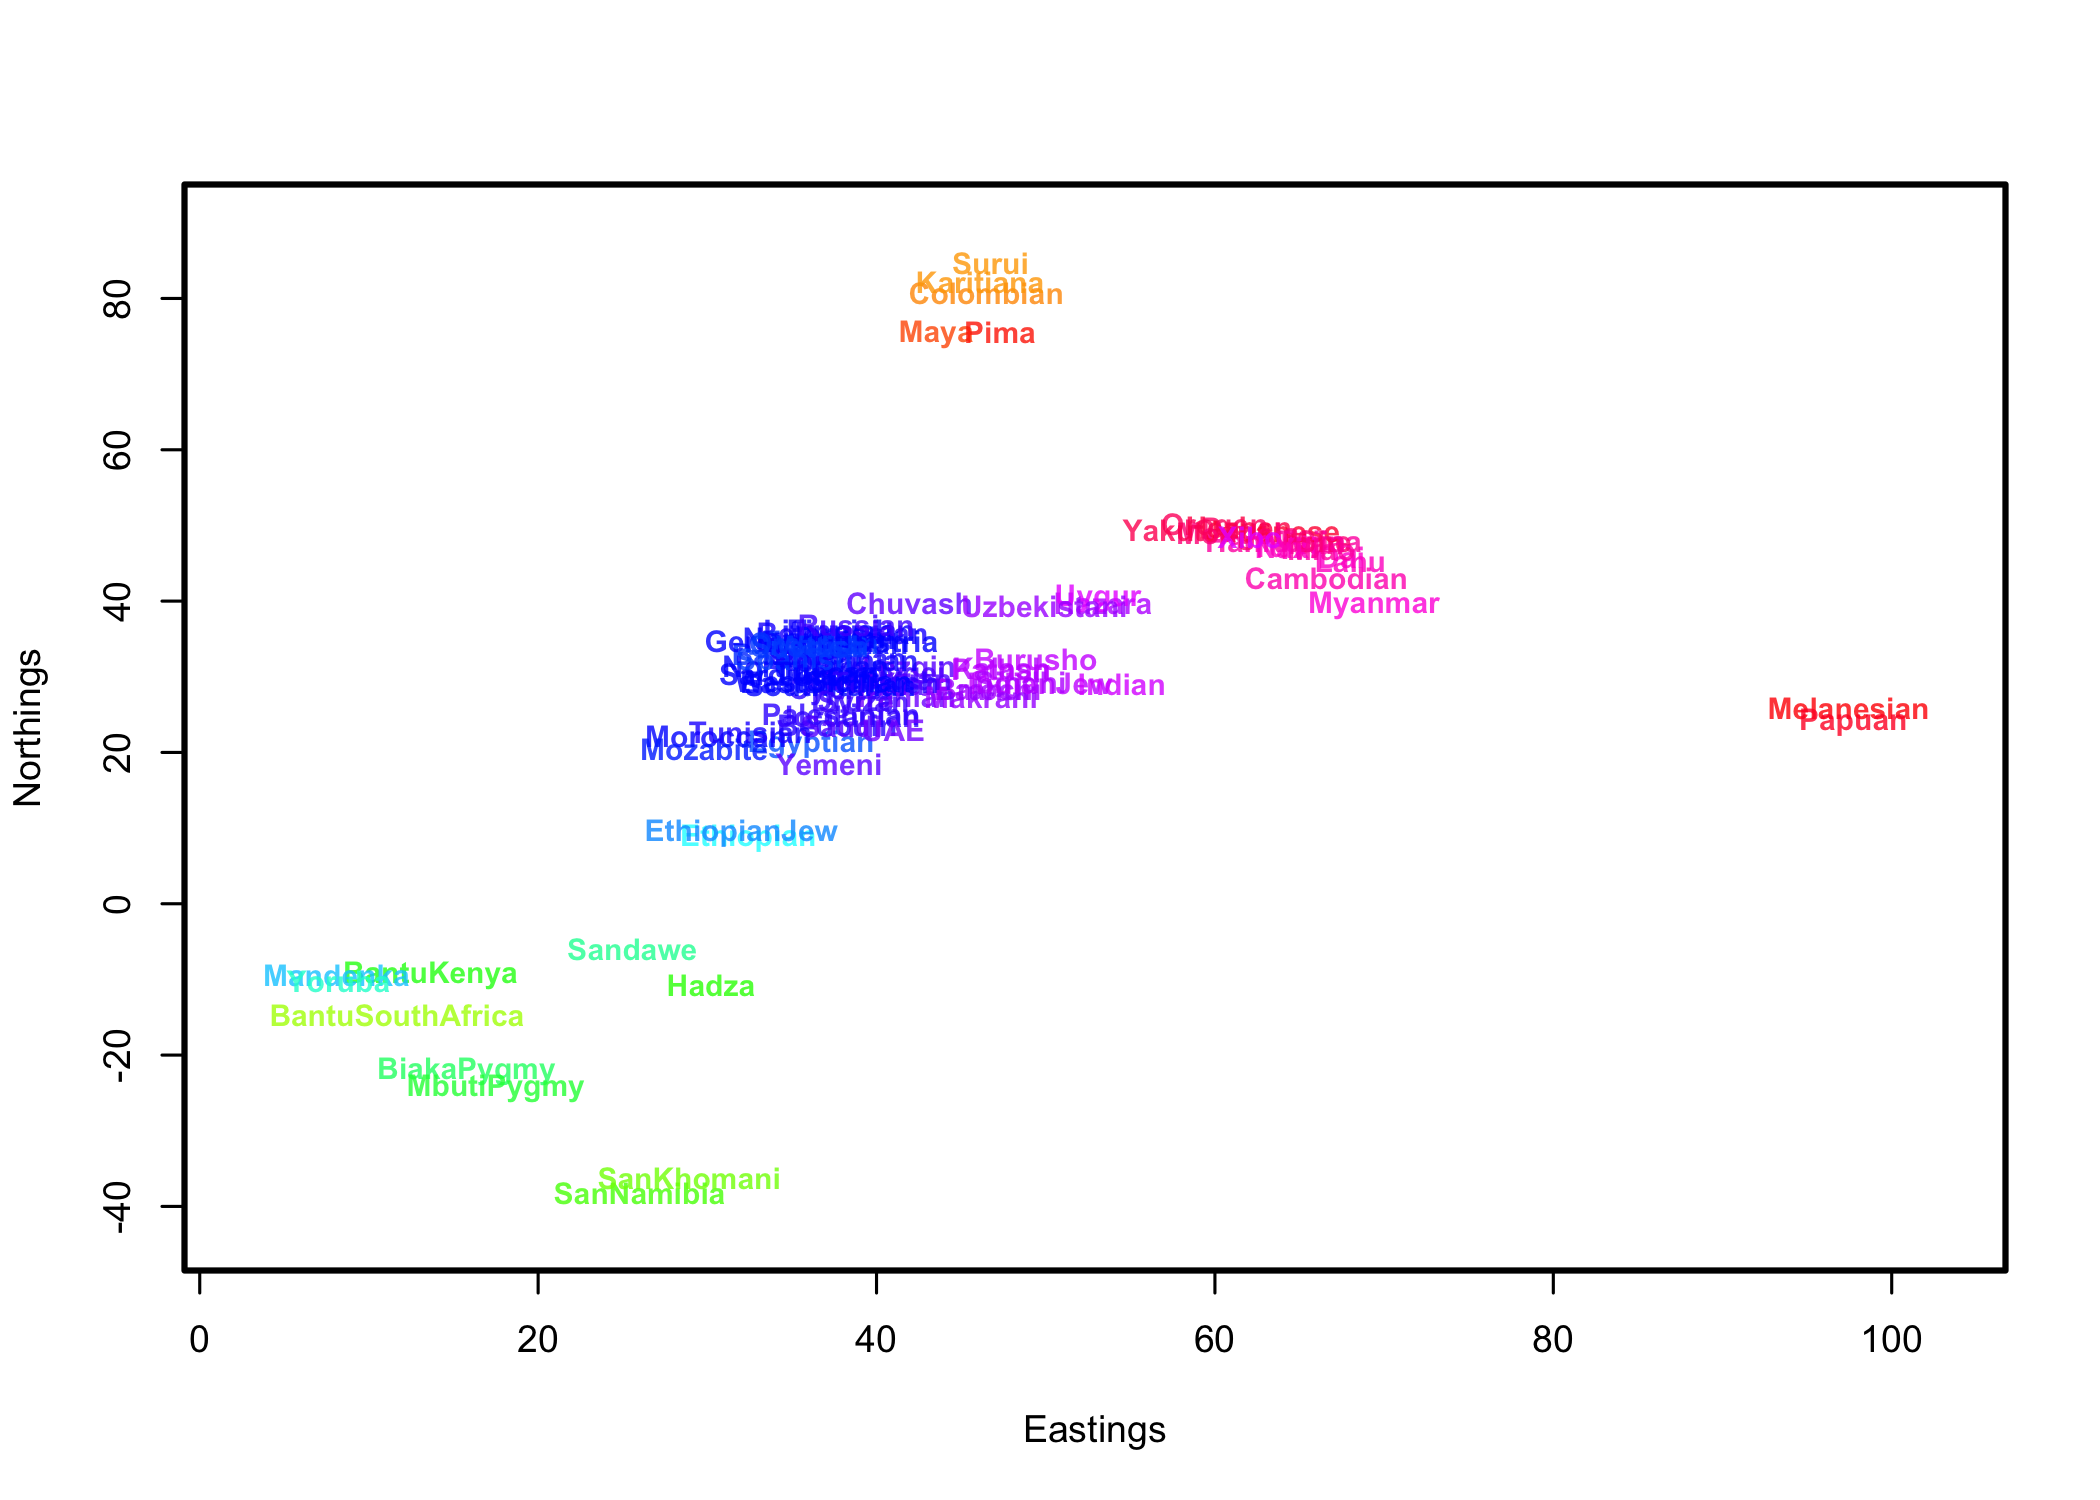
\includegraphics[width=2.8in,height=2.3in]{figs/globetrotter/globe_NoAd_map.png}}
%		\subcaptionbox{Closeup of African populations \label{globe_africa_noad_map}}
%			{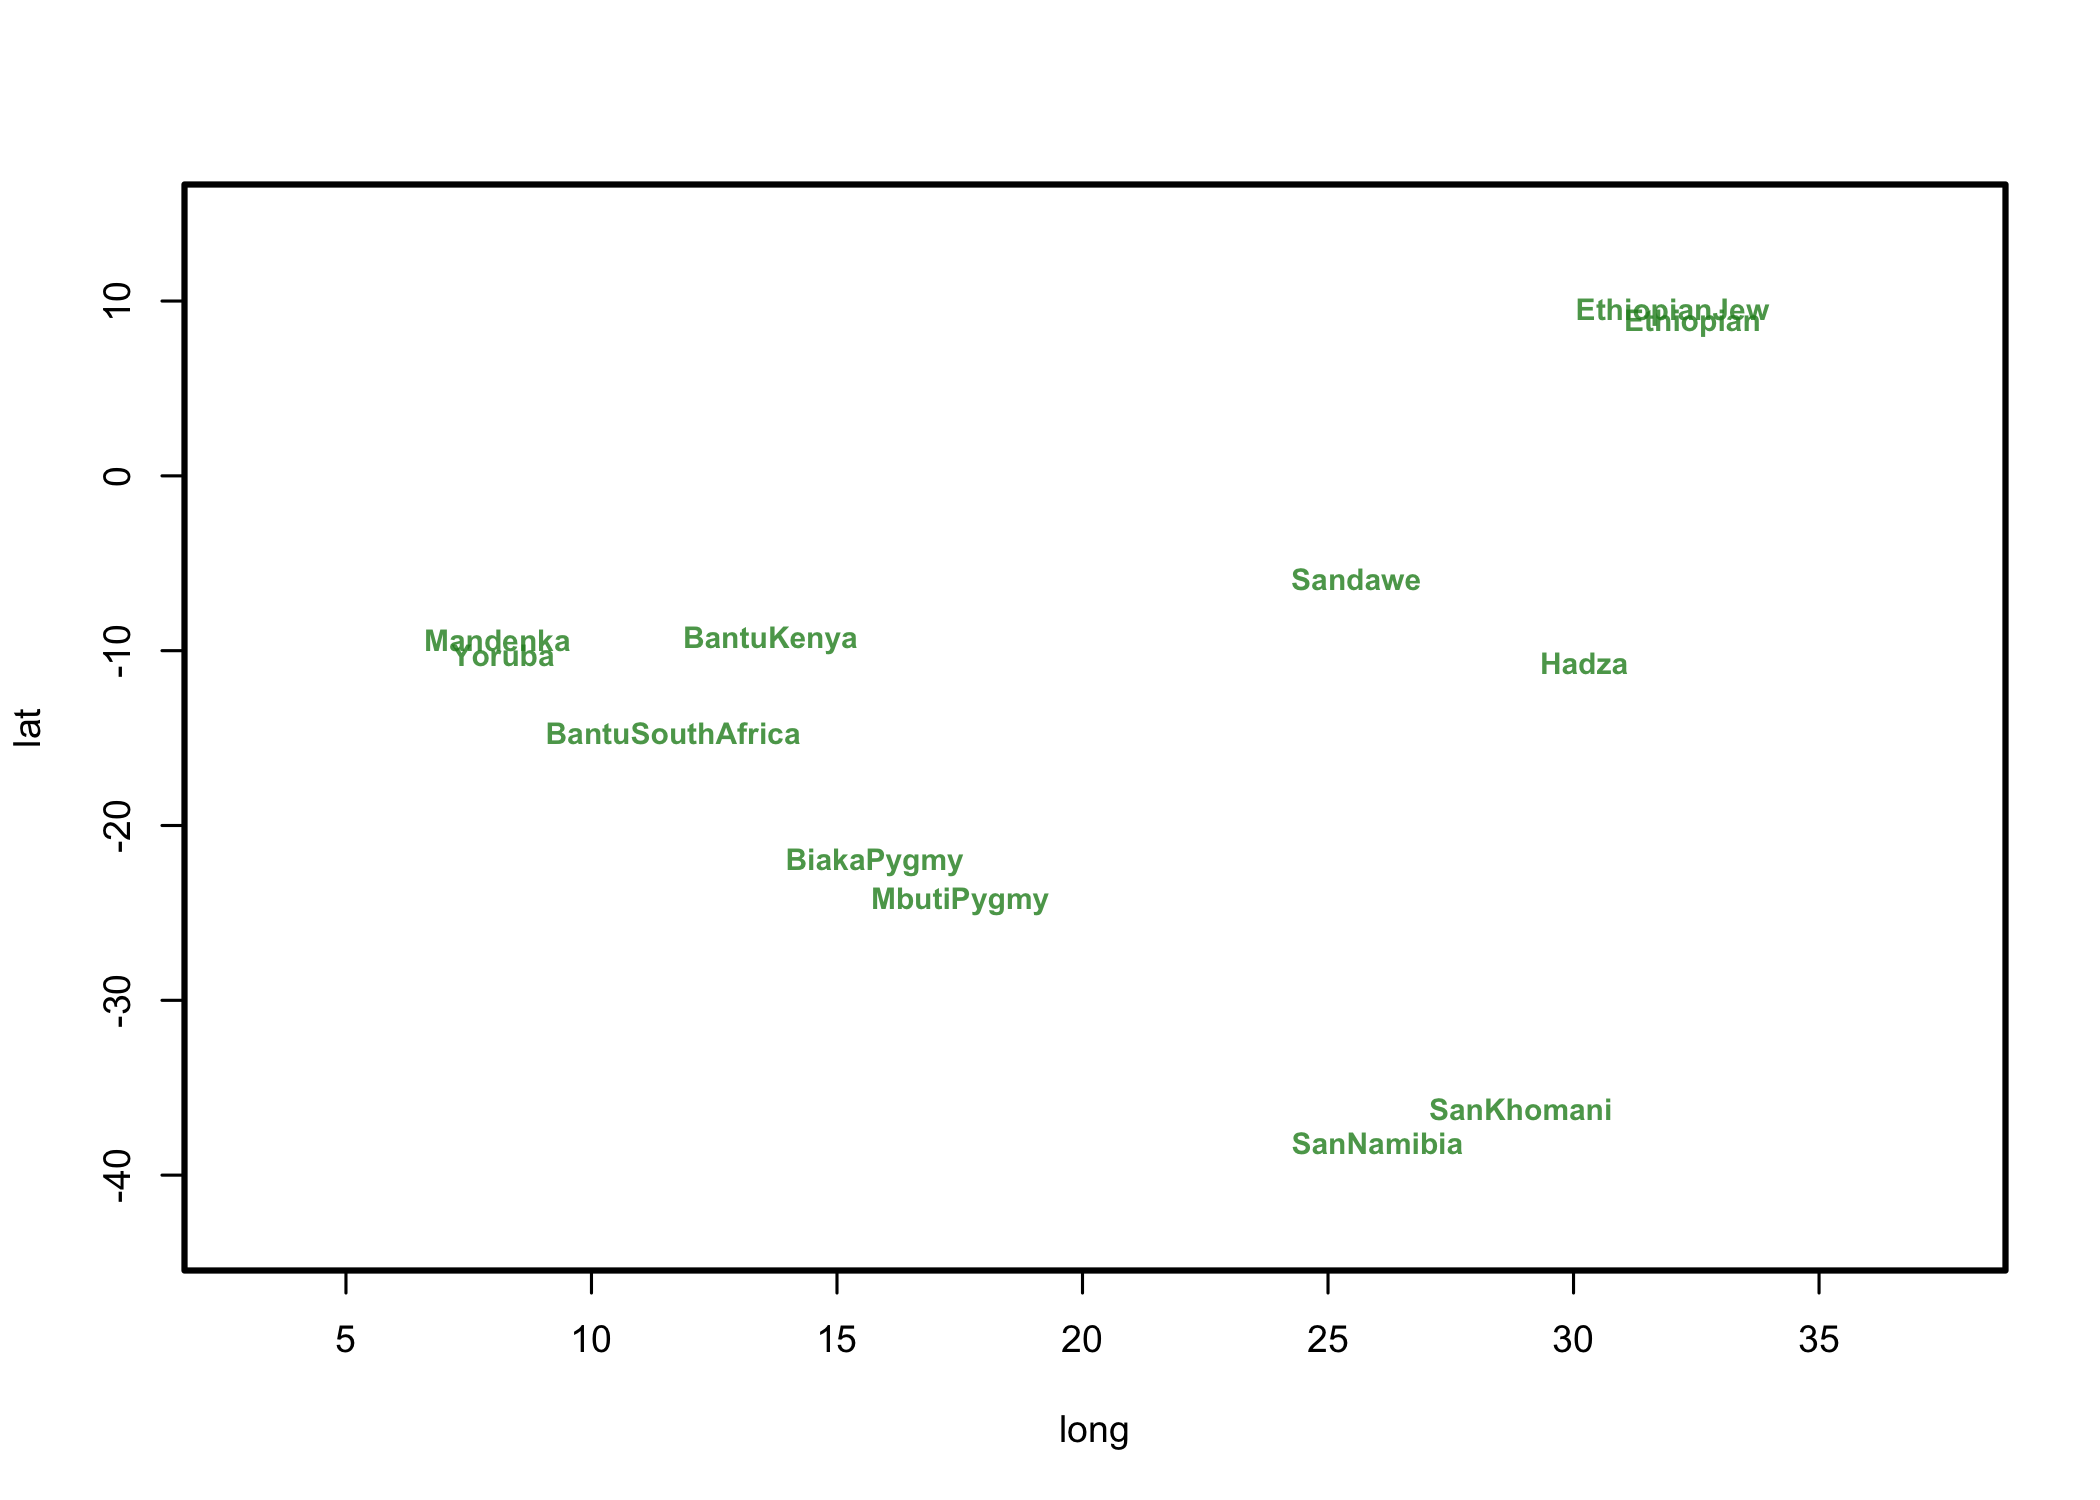
\includegraphics[width=2.8in,height=2.3in]{figs/globe_Africa_NoAd_map.png}}
%		\subcaptionbox{Closeup of non-Africa populations \label{globe_notafrica_noad_map}}
%			{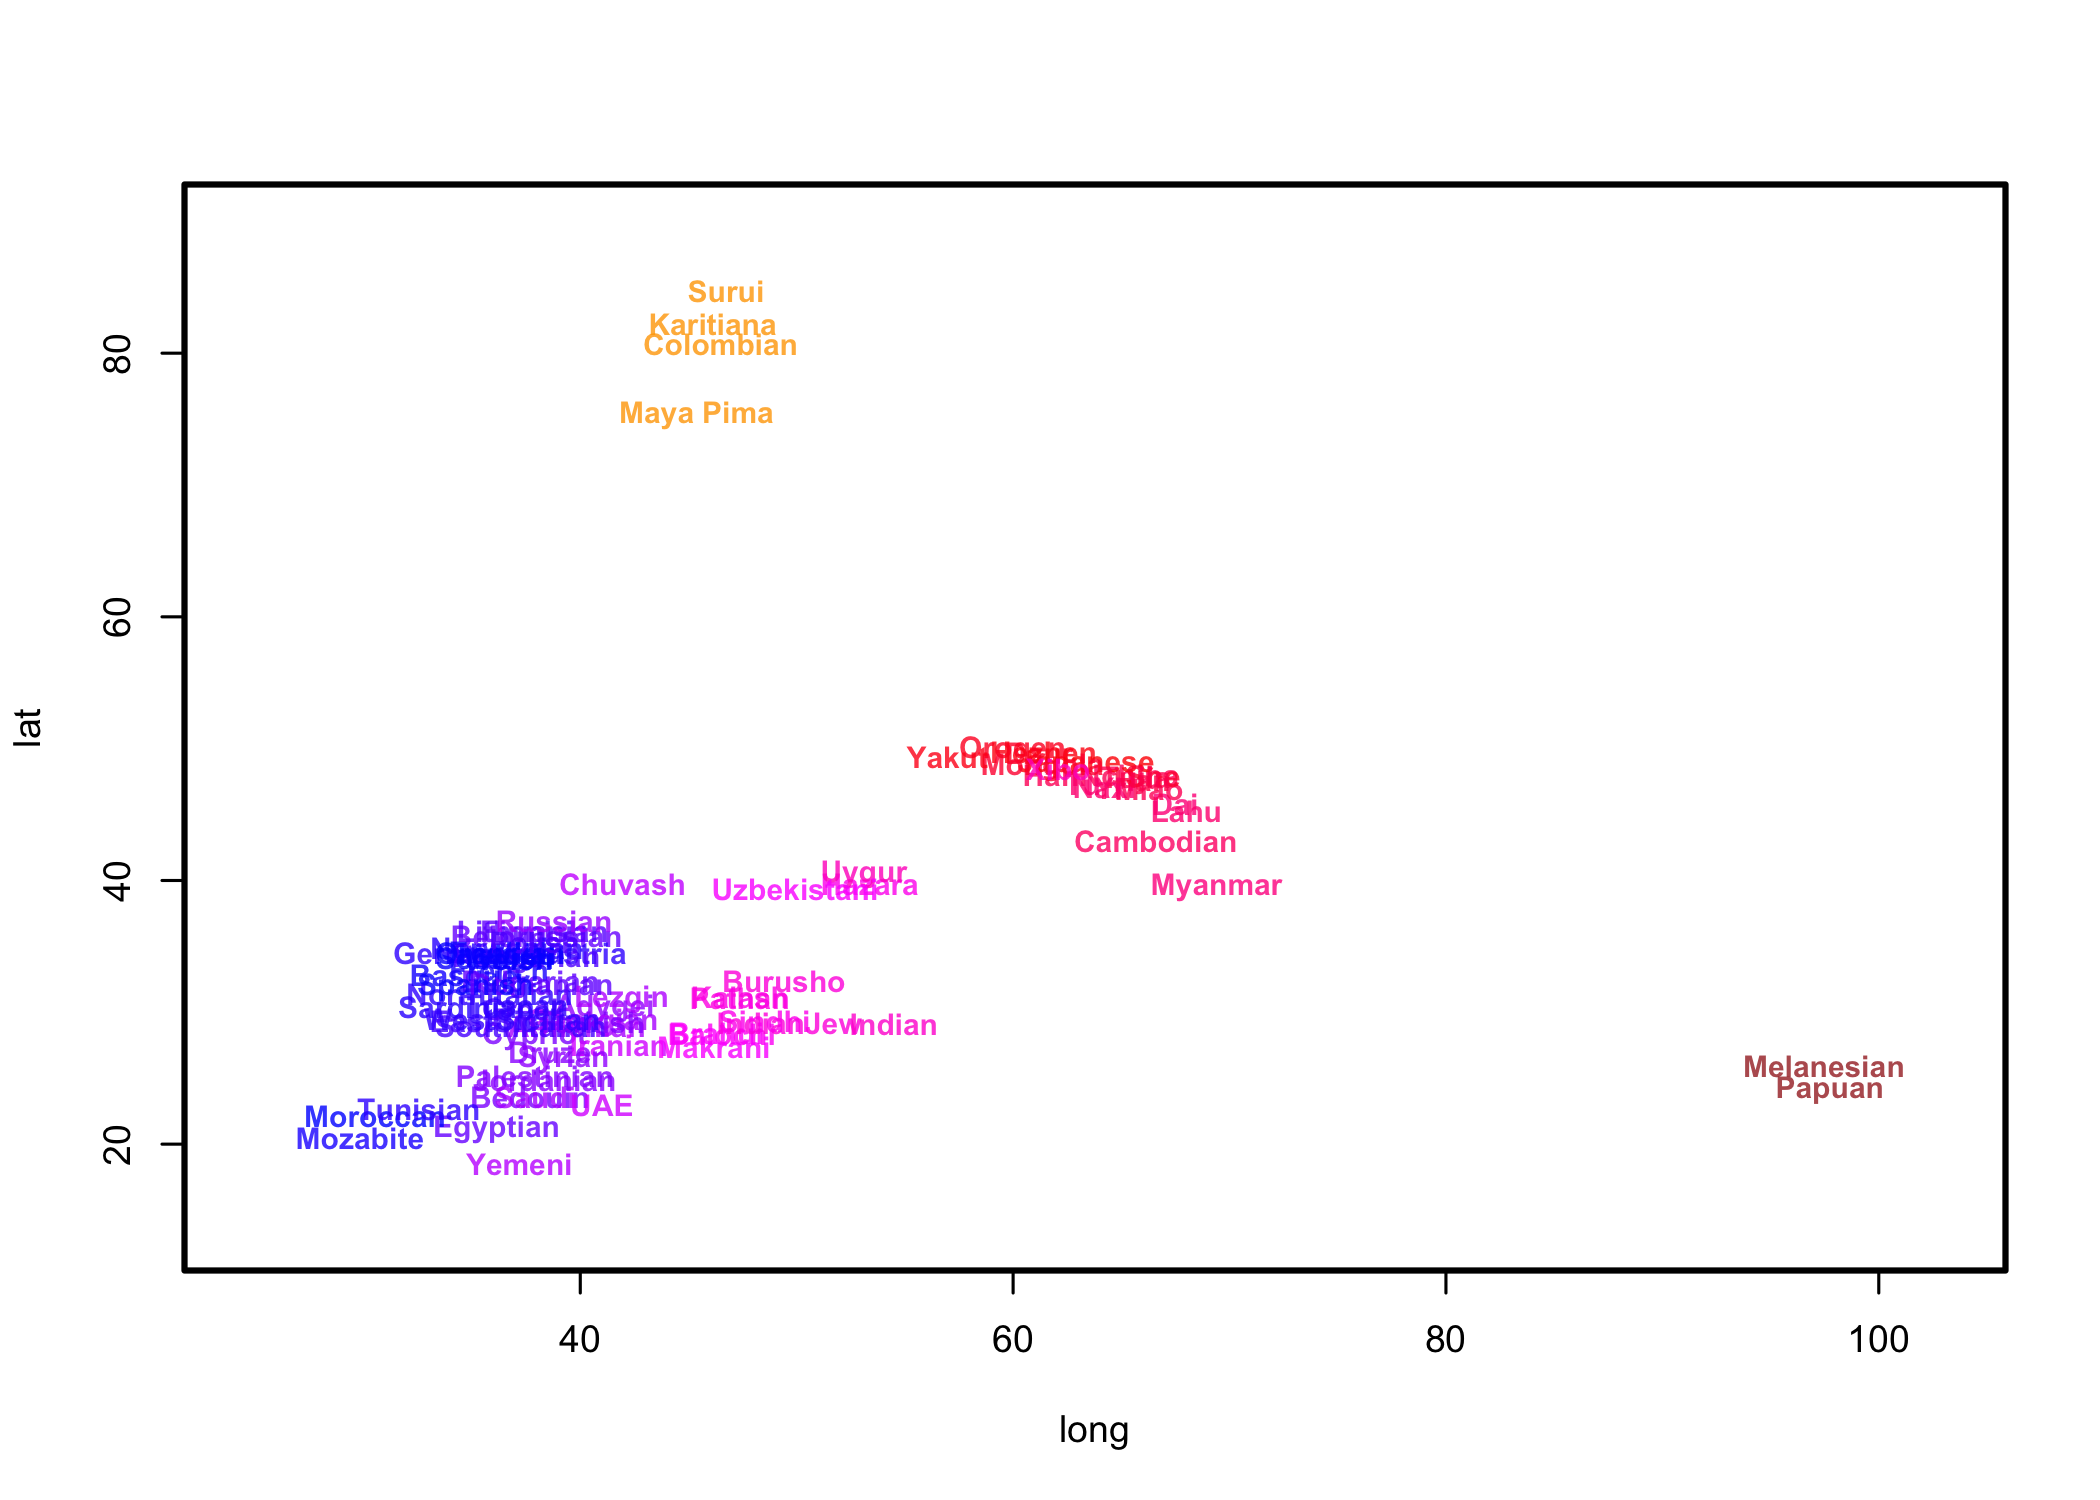
\includegraphics[width=2.8in,height=2.3in]{figs/globe_Eurasia_Americas_Oceania_NoAd_map.png}}
		\subcaptionbox{Closeup of Eurasian populations \label{globe_eurasia_noad_map}}
			{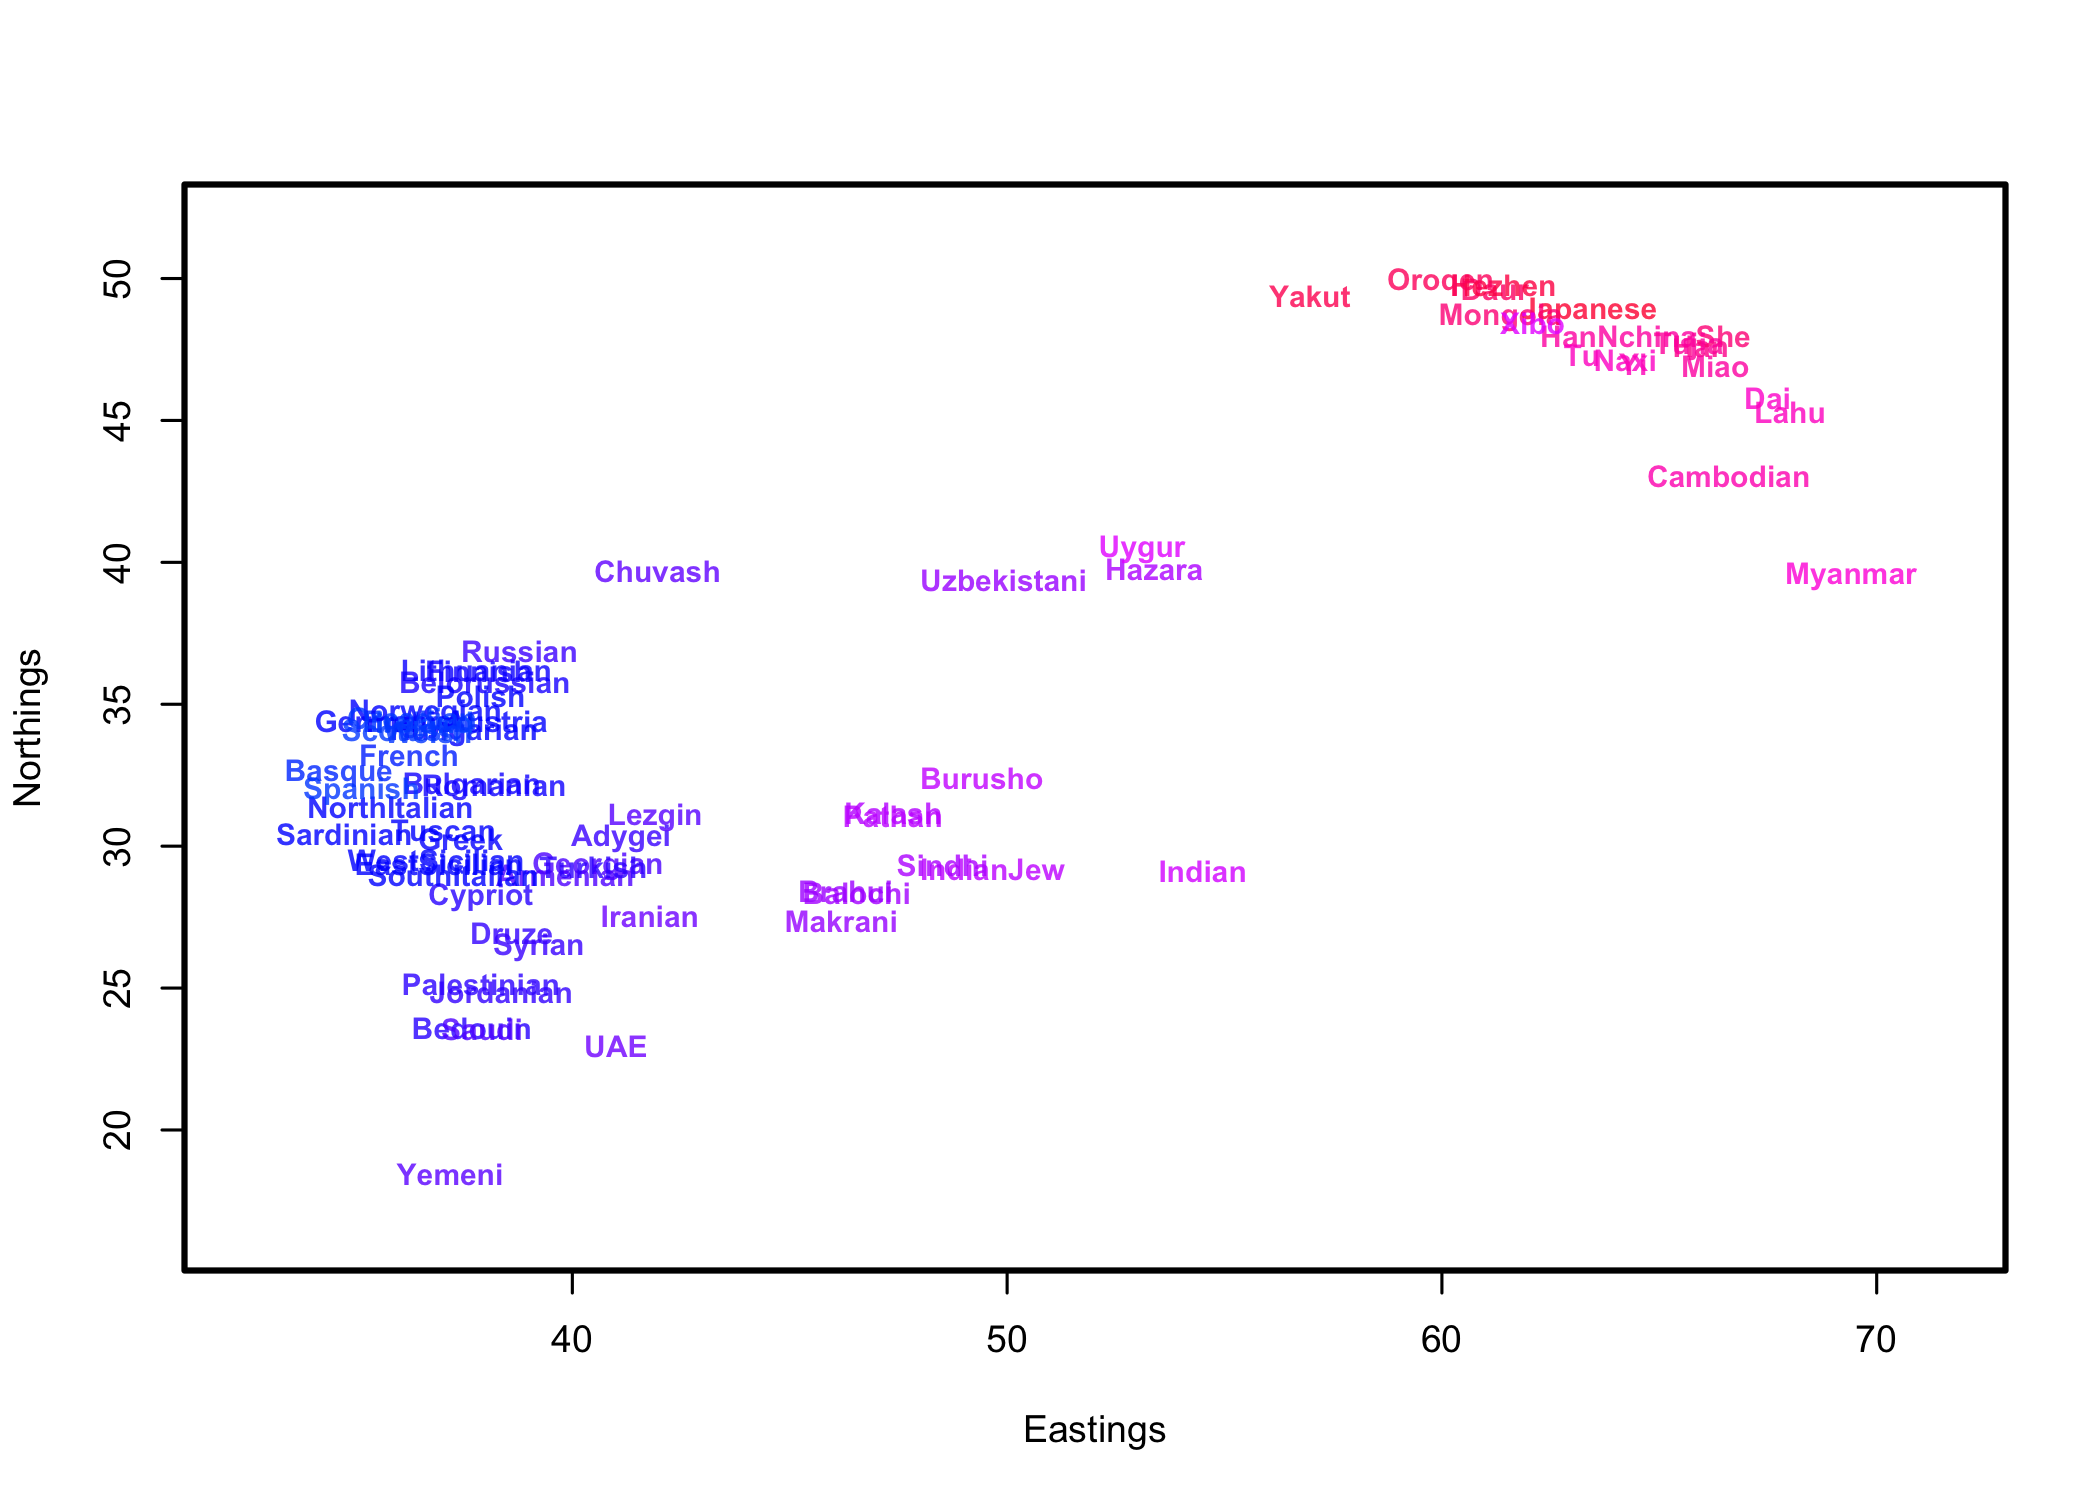
\includegraphics[width=2.8in,height=2.3in]{figs/globetrotter/globe_Eurasia_NoAd_map.png}}
	\caption{Map of human populations, inferred without admixture. (a) complete map; (b) close up of Eurasian 
populations.}\label{sfig:globe_noad_maps}
%(b) close up African populations; (c) close up of all non-African populations;
\end{figure}

We also recover evidence for several major population expansions and colonization routes in human pre-history.  We can see evidence of these expansions by examining the relationship between observed and estimated pairwise distance between the daughter populations of a putative expansion event.   As can be seen in \ref{sfig:lattice_scenarios}\subref{expansion_inference}, populations that have recently expanded on the landscape are less differentiated both from each other and from their parent population than would be expected from their geographic separation, and this fact is reflected in the decreased ratio between estimated and observed pairwise distances between members of an expansion event.

In the SpaceMix analysis of the human genetic data, the scale of inferred inter-population distance within Africa is much greater than that between any other group (see Fig. \ref{sfig:globe_noad_distcomp}), and the slope of the relationship between observed and estimated distances between populations on each continent decays with distance from Africa.  This pattern is consistent with a history of human colonization events characterized by serial bottlenecks, including an out-of-Africa expansion, an expansion into East Asia, and twin expansions into the Americas and Oceania (REFS) .  In addition, we see that both the populations in the Americas and in Oceania cluster close to the East Asian populations, but that the two clusters are on opposite sides.  The proximity of these groups to the East Asians represents the fact that both groups were ancestrally East Asian (REF?), but that the expansion events induced independent drift trajectories in both waves of colonization.  

We also see intriguing evidence for potential admixture in the placement of the Chuvash, Uzbekistani, Hazara, and Uygur populations, which choose locations intermediate between Europe and East Asia, as well as in the placement of the Moroccan, Mozabite, and Ethiopian populations, which are choosing locations between the western Eurasian cluster and the African cluster.  To investigate possible patterns of admixture further, we ran a SpaceMix analysis in which we estimated, for each population, a location, a source of admixture, and the magnitude of that admixture.
Ran the method with admixture


In figure XXX we show   . Some arrows are hard to see, but still likely biologically meaningful for example the Maya draw from  

The iggest change is the positioning of Sub-Saharan African samples with respect to the rest of the world.  Including admixture means that samples that fell intermediate between  Sub-Saharan Africa and North Africa and the middle east now move closer to one or the other.  The Ethiopian and Ethiopian Jewish samples move to be relatively closer to the Sub-Saharan samples than the North African samples (mention Hadza and Sandawe).  While the North African populations (Egyptian, Tunisian, Morocan, Mozabite) move to join the middle eastern populations (positioning in rough accord with their sampling location along north-Africa). The relatively large distances between these groups reflects the fact that ,,,

Now instead of occupying an intermediate position the two Ethiopian samples draw a substantial proportion of their ancestry ($\sim 40\%$) from close to where the Egyptian sample has positioned itself in the the middle East cluster. The Sandawe population also draw a substantial portion of their ancestry from the middle east cluster.  Where's the Hadza going? Reciprocally, our North African samples (Egyptian, Tunisian, Morocan, Mozabite), having moved to join the middle eastern populations draw ancestry from close to the Ethiopian samples. Interestingly the Bantu South African sample, though the move to join the other Bantu populations, draws admixture from close to the (Kohi?) San populations. This is consistent with previous signals ....

SanKhomani draws admixture from near syria.

The middle eastern sample () draw admixture from close to the location chosen by the Ethiopian samples, close to where the North African samples draw admixture from. It seems potentially likely that this spread of populations represents North African influence. 

The Sindi, Makrani and Brahui draw admixture from close to the location of the Bantu samples.Balochi and Kalash draw admixture from some distance away from African populations.

Europe, not much but spanish, East and West Sicilian samples all draw small amounts of admixture from close the Ethiopian samples (presumably north African ancestry component). 

The other dominant signal of admixture is between East and West Eurasia. The majority of samples maintain their relative positions within each of these groups. However, the Uzbekistani and Hazara samples move to be closer to the East Asian samples, while drawing a substantial admixture proportion from close to the Georgian and Armenian samples have located themselves. While conversely the  Uyrgur sample moves to be close to the Burusho, Kalash, and Pathan. The Tu (who locate to East Asia) draw small amount of ancestry from close to where the Uygur have positioned themselves.
The Chuvash move close to Russian and Lithuanian, drawing admixture from close to the Yakut; the Turkish sample also draws a smaller amount of admixture from here. There are a number of other East-West connections the Russian, Adygei samples have admixture from a location ``north'' of our East Asian samples.  Cambodia draws admixture from close to the Eygptian sample (also seen by Treemix). 


Need to work out what to say about folks drawing admixture away from everyone else.

Burusho draws admixture away from everyone.
Xibo from weirdly ``north west'' of Europe.  

Pathan draws from where india also draws admixture from.








\begin{figure}
	\centering
		{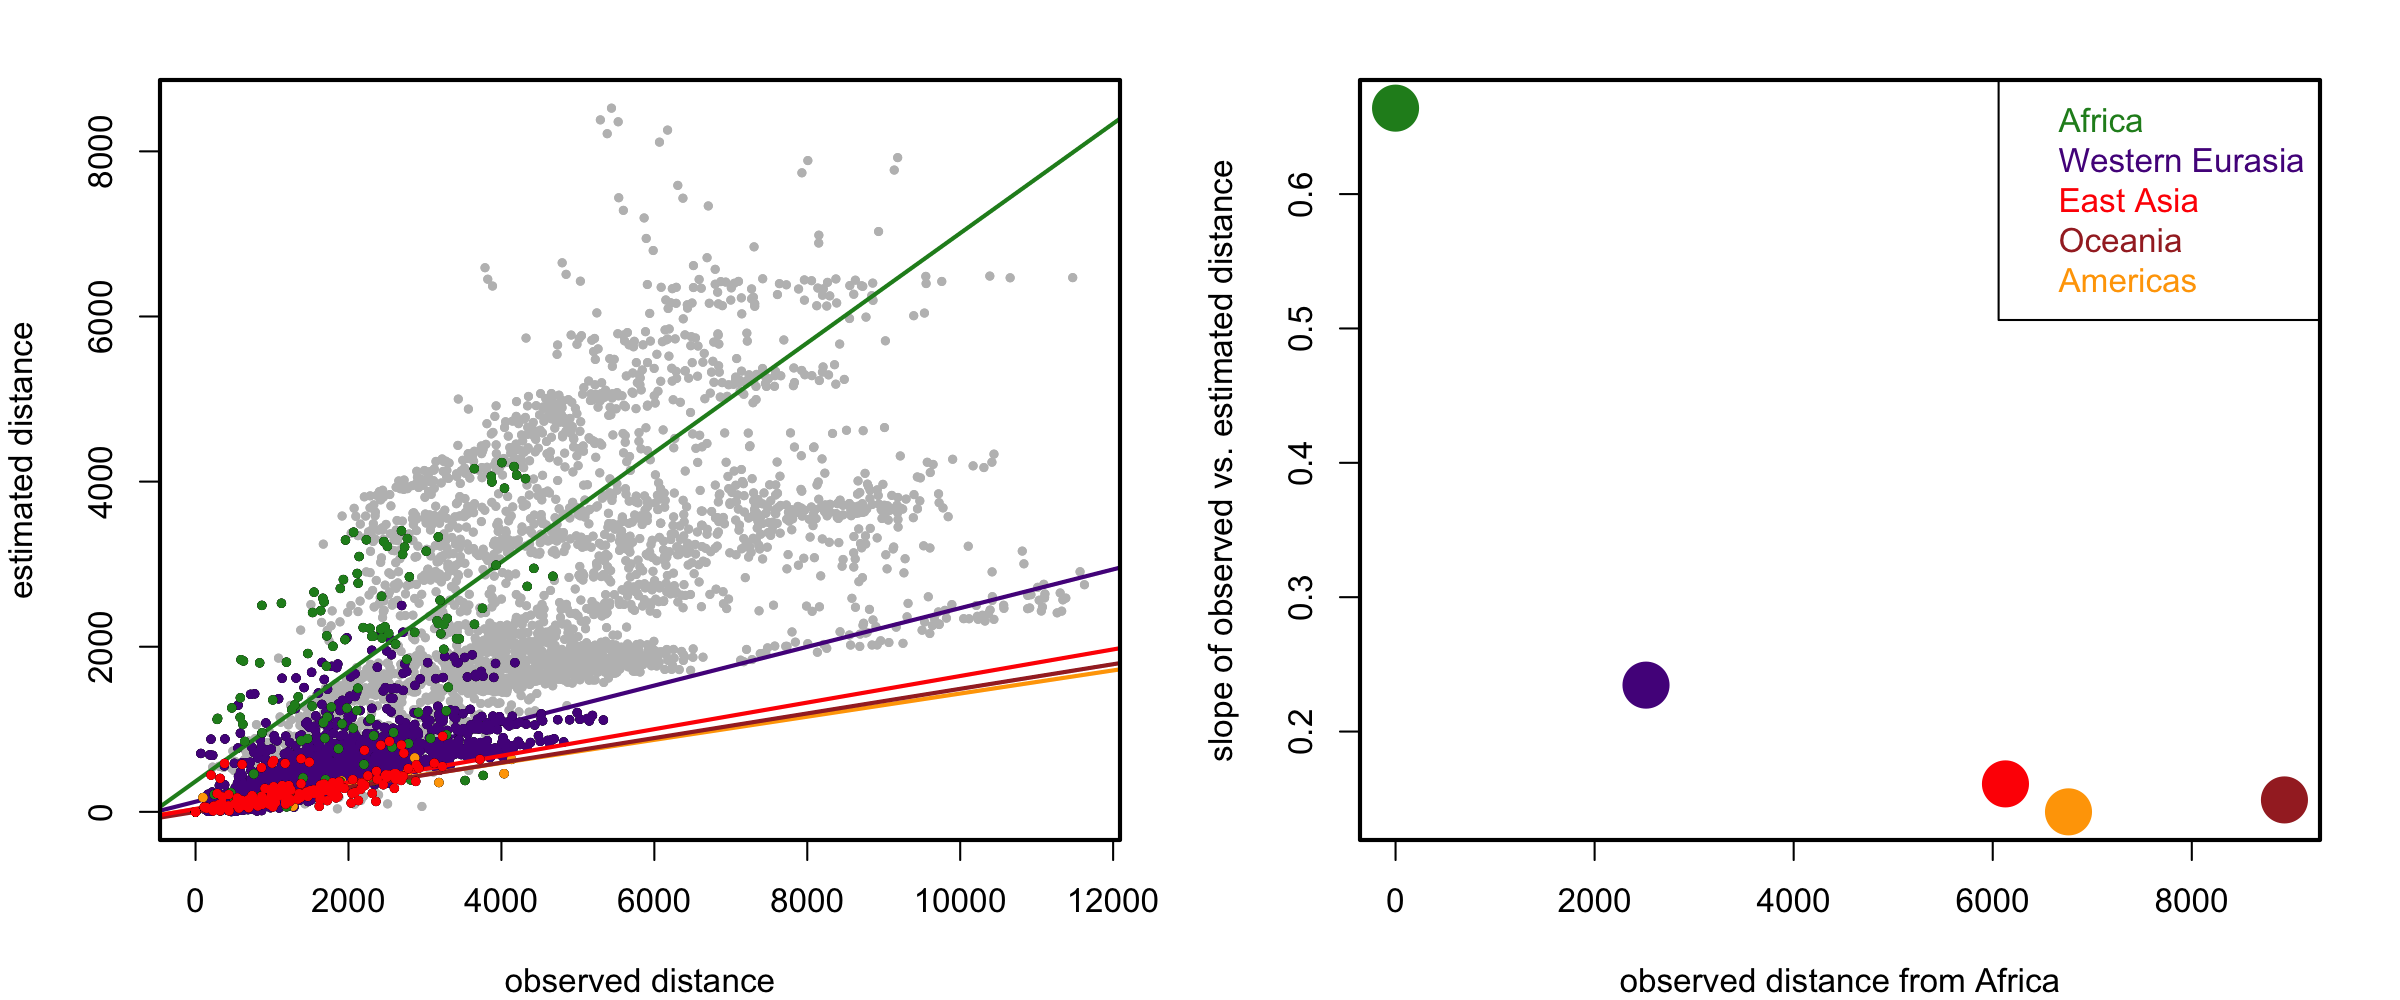
\includegraphics[width=6in,height=2.5in]{figs/globetrotter/globe_NoAd_dist_decay.png}} %globe_NoAd_dist_compare.png
	\caption{Comparison of observed distance to estimated distance between human populations, colored by continent from which populations were sampled (i.e. - two populations sampled from Africa are green).  Eurasia is divided into Western Eurasia and East Asia.}
\label{sfig:globe_noad_distcomp}
\end{figure}

\begin{figure}
	\centering
		\subcaptionbox{Inferred map of human populations \label{globe_all_ad_map}}
			{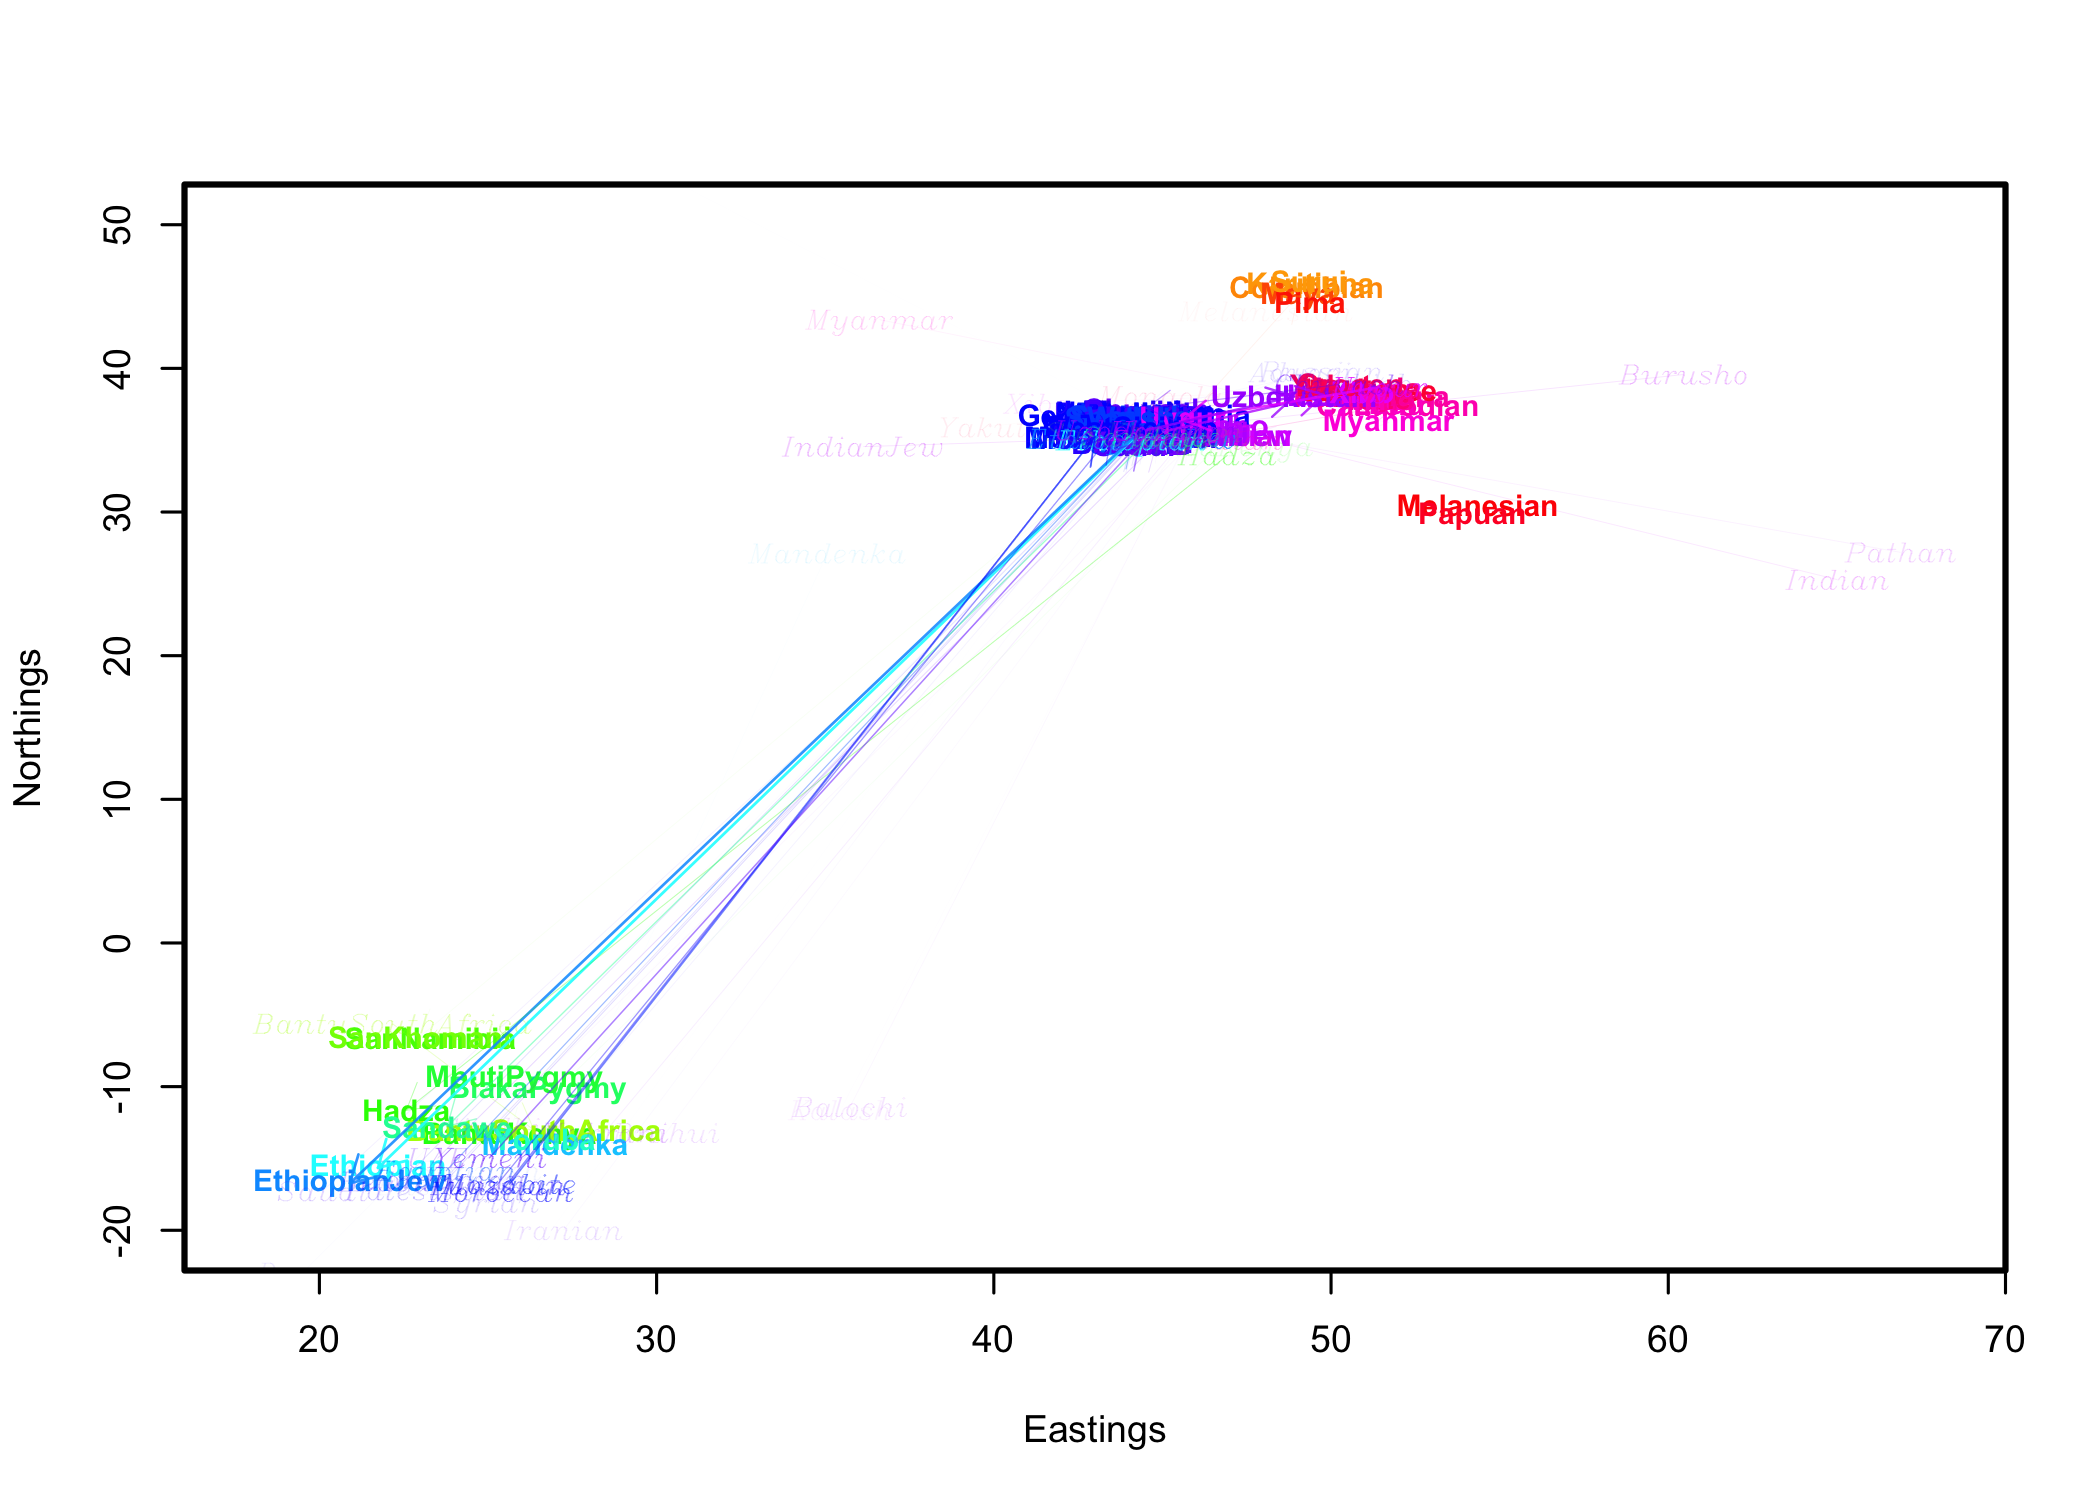
\includegraphics[width=2.8in,height=2.3in]{figs/globetrotter/globe_Ad_map.png}}
%		\subcaptionbox{Closeup of African populations \label{globe_africa_noad_map}}
%			{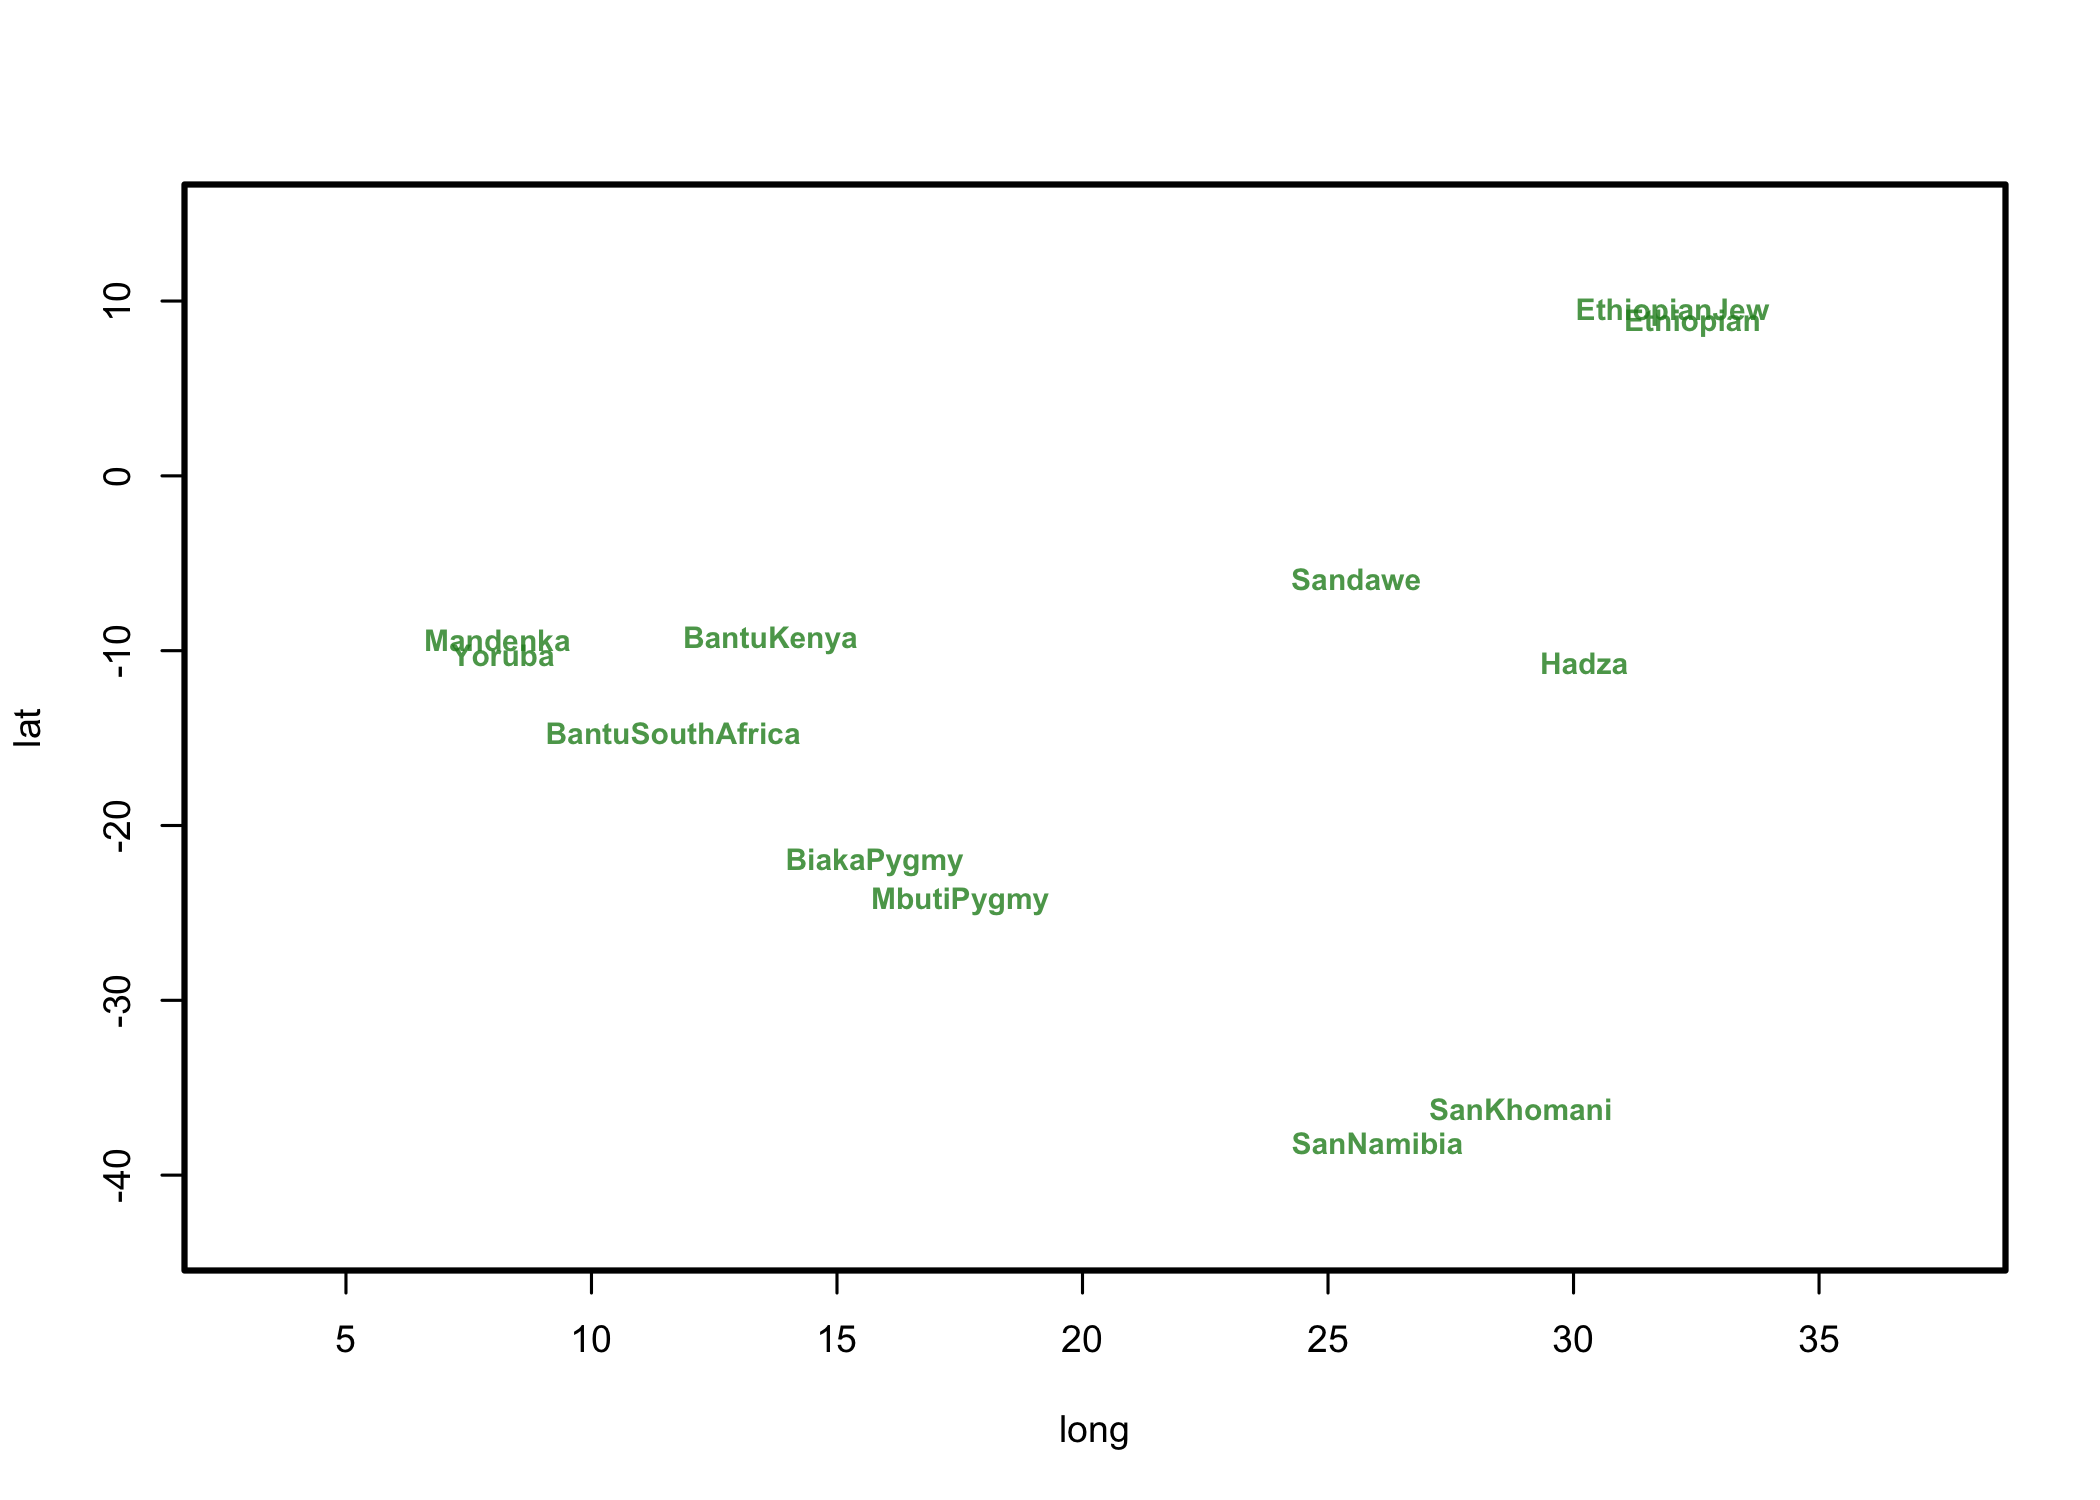
\includegraphics[width=2.8in,height=2.3in]{figs/globe_Africa_NoAd_map.png}}
%		\subcaptionbox{Closeup of non-Africa populations \label{globe_notafrica_noad_map}}
%			{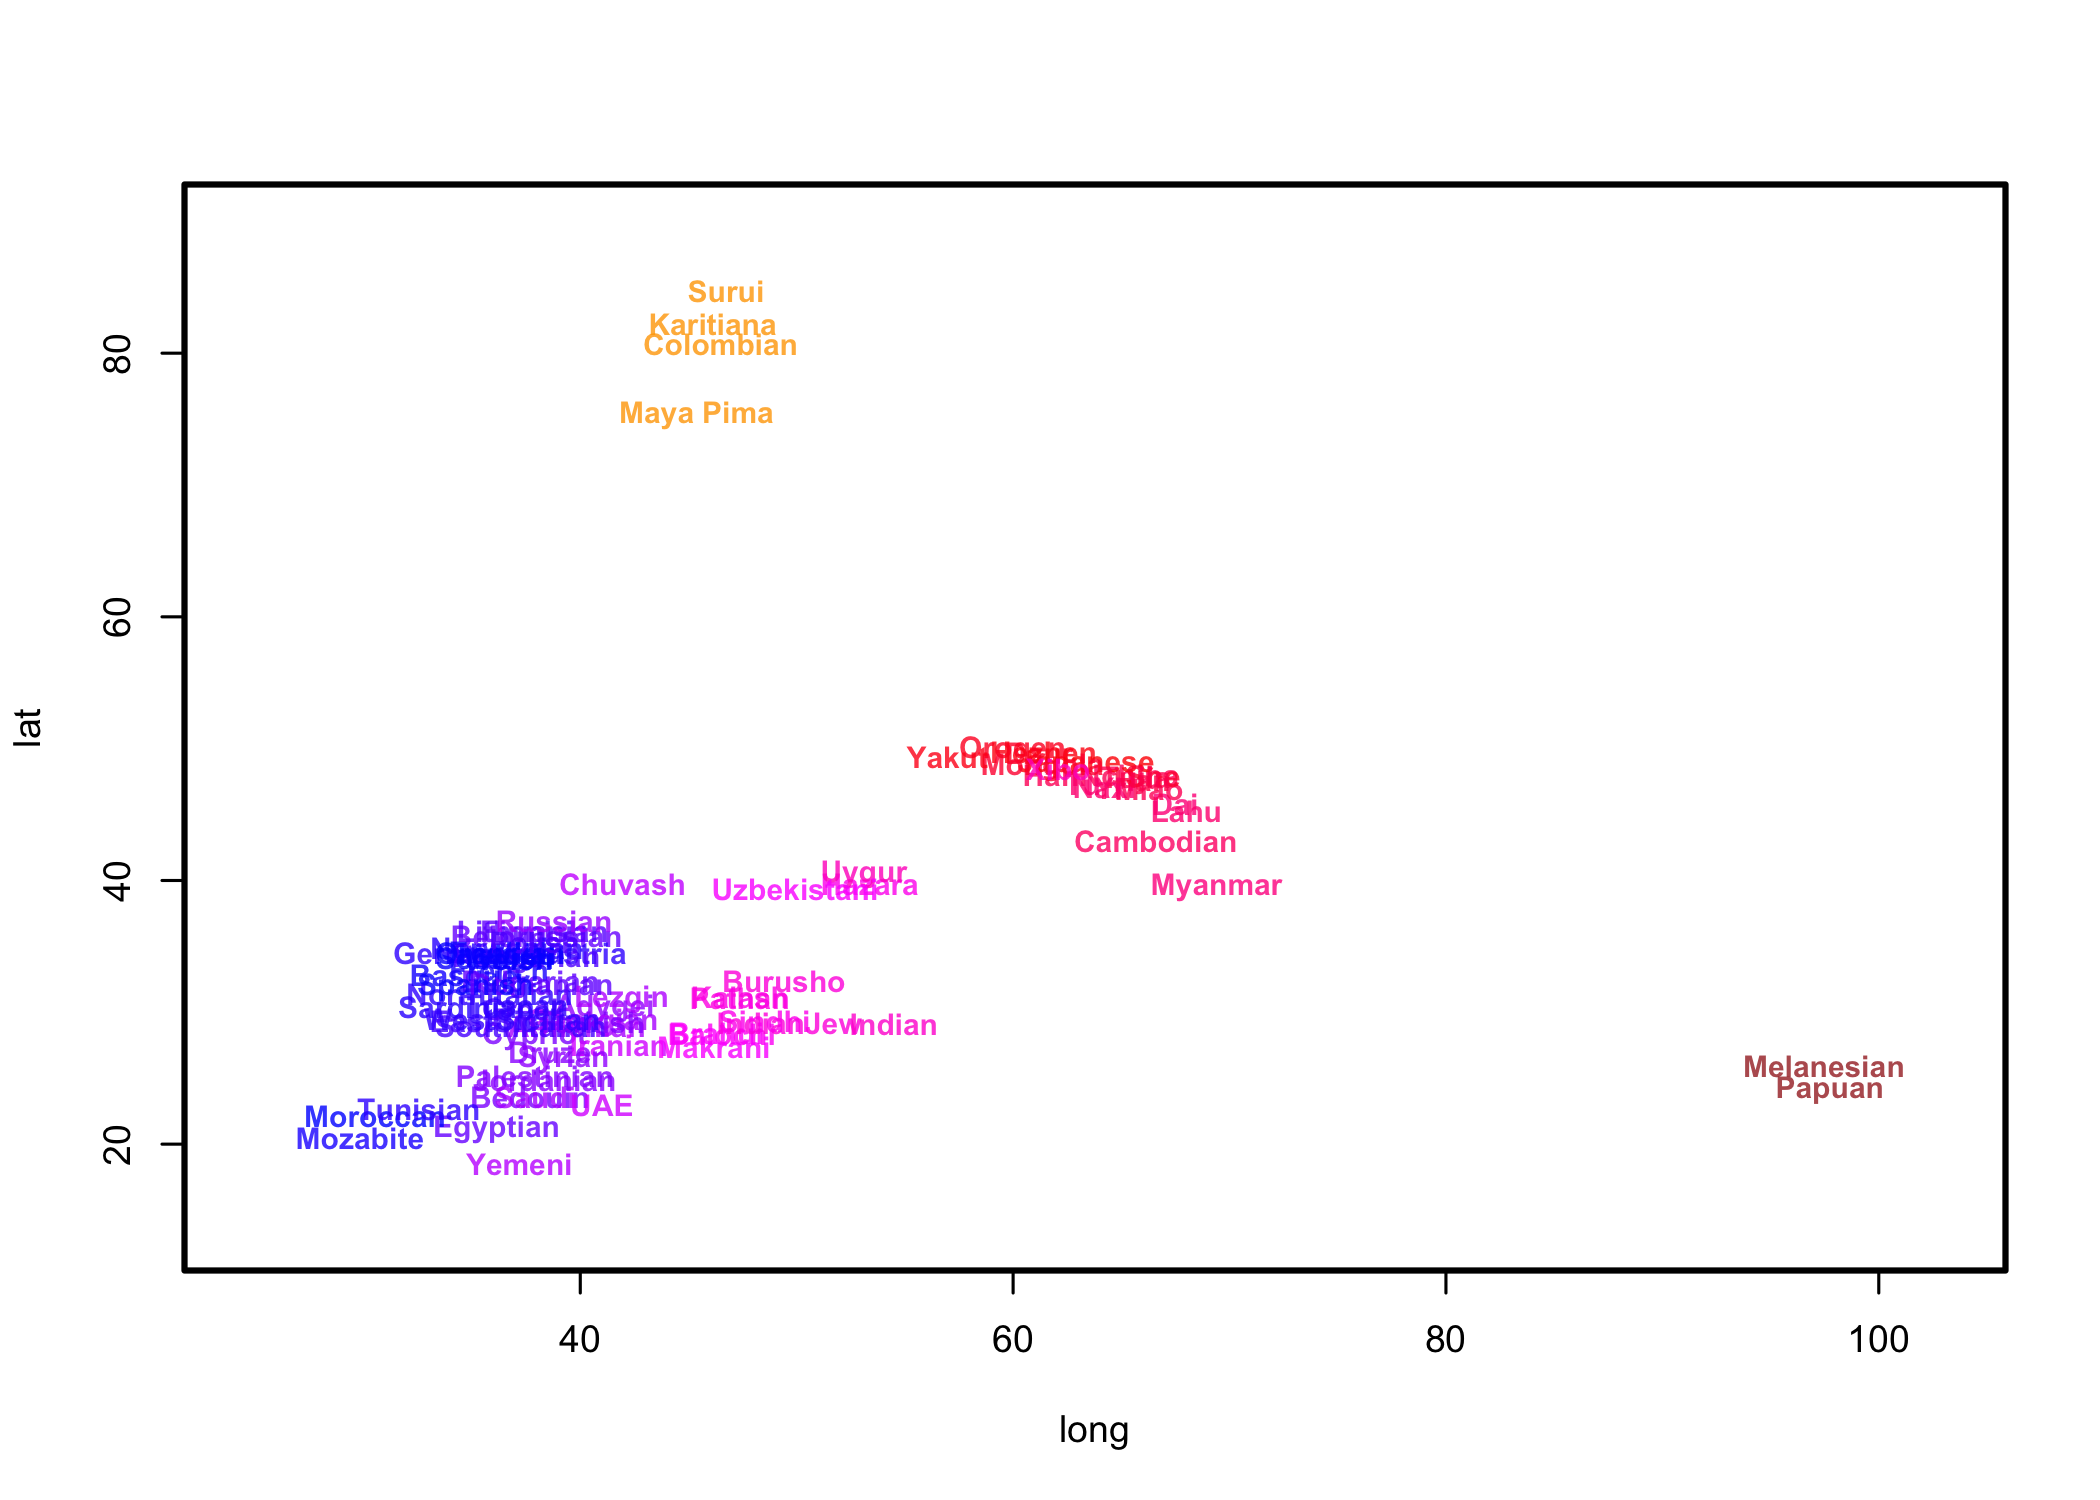
\includegraphics[width=2.8in,height=2.3in]{figs/globe_Eurasia_Americas_Oceania_NoAd_map.png}}
		\subcaptionbox{Closeup of Eurasian populations \label{globe_eurasia_ad_map}}
			{\includegraphics[width=2.8in,height=2.3in]{figs/globetrotter/Eurasia_Ad_map.png}}
	\caption{Map of human populations, inferred with admixture. (a) complete map; (b) close up of Eurasian populations.}\label{sfig:globe_ad_maps}
\end{figure}


\section*{Conclusion}
In this paper we have presented blah blah blah.  We believe this represents an advance over previous methods because blah blah blah.  This method can be used to answer a variety of empirical questions, including blah, blah, and blah, and also serves as an intuitive data visualization tool.

\section*{Future Directions}

spatiotemporal model

spatialSTRUCTURE

\section*{Methods}
As described above, we have developed an algorithm, called SpaceMix, that uses the standardized sample allele frequency covariance and the the likelihood equation in Eqn. \eqref{eq:admixed_post_prob} to simultaneously estimate the posterior distribution of the population locations, $G'$, their sources of admixture, $\identifyadmixsource{G}$, their admixture proportions, $w$, their independent drift parameters, $\eta$, and the parameters of the model of isolation by distance, $\vec{\alpha}$.  The inference procedure has two principal components: (1) the derivation of the standardized sample allele frequency covariance matrix, and (2) a Markov chain Monte Carlo algorithm that samples parameter values from the posterior distribution.  Here, we describe these procedures in detail.

\subsection*{Deriving the standardized sample covariance}
In the section on the normal approximation to drift, we describe how genetic drift - serial binomial sampling of allele frequencies through time - can be approximated as normally distributed change in allele frequencies around some ancestral mean, which we call $\epsilon_A$.  Under this normal approximation, the frequency of an allele in daughter population $B$ (sampled at some later point in time) can be described by the following equation,
%
\begin{equation}
\label{eq:normal_drift}
\epsilon_B \sim N(\epsilon_A,\delta_B(\epsilon_A)(1-\epsilon_A)),
\end{equation}
%
where $\delta_B$ is the amount of drift separating $A$ and $B$.  This drift parameter is approximately equal to $\frac{t}{2N_e}$, where $t$ is time in generations separating $A$ and $B$, and $N_e$ is the constant effective population size.  Note that the binomial variance term in the normal variance in \eqref{eq:normal_drift} ignores the fact that the drift variance will change from generation to generation due to changes in the frequency of $\epsilon$ within a population over time.  Note also that this approximation works best for alleles at intermediate frequency, which are less likely to be lost or fixed during the interval separating the sampling of $A$ and $B$.  However, if the extent of drift is sufficiently limited (time scales are short or population sizes are large), the approximation of inter-generational binomial sampling to Brownian motion is good.  

Among populations, the differentiating process of drift is counteracted by the homogenizing force of migration, so that populations with higher levels of historical or ongoing migration can be thought of as having more shared drift, i.e. stronger covariance in their allele frequency deviation around the ancestral (or global) mean.  Following Tobler's law (``everything is related to everything else, but near things are more related than distant things), we assume that the rate of migration between populations is inversely proportional to their geographic separation, such that the covariance in allele frequencies across loci between a pair of samples separated by a small distance is greater than that between a pair separated by a large distance.  

We model the population frequencies at a locus as multivariate normal (MVN) with mean $\epsilon$ and covariance matrix $\epsilon(1 - \epsilon)\Omega$.  The multivariate normal distribution offers a natural statistical framework for describing this covariance, which may be straightforwardly modeled as a parametric function of any pairwise distance variable.

We wish to model the covariance between populations as the result of a spatial process, in which migration rates between nearby populations are higher than between distant ones, so that a population has higher covariance with a close neighbor than with a more distant population.  We choose as the form of our parametric covariance matrix a simple and flexible model, with an exponential decay of allele frequency covariance with geographic distance (Wasser et al 2004, Bradburd, Ralph, and Coop 2013).  The covariance between population allele frequencies in populations $i$ and $j$ is 
%
\begin{equation}
%\label{eq:spatial_covariance}
\Omega_{i,j} = \frac{1}{\alpha_0} \text{exp} \left(	\left( \alpha_1D_{i,j} \right)^{\alpha_2} \right) \text{,}
\end{equation}
%
where $D_{i,j}$ is the geographic distance between population $i$ and $j$ (and therefore a function of their locations, $G_i$ and $G_j$), $\alpha_0$ controls the within-population variance, or the covariance when distance between points is 0 (the sill of the covariance matrix),  $\alpha_1$ controls the rate of the decay of covariance per unit pairwise distance, and $\alpha_2$ determines the shape of that decay. While previously we and others have used a logit link function combined with binomial sampling to model the sample frequencies \citep{Wasser, Bradburd}, here we chose to treat these standardized frequencies $\hat{f}_{\ell}$, as multivariate normal across populations \citep[]{Treemix}. To accommodate the effect of finite sample size we introduce ``nuggets'' of population-specific variance terms, on the diagonal of allelic covariance matrix,which accommodate the effects of both sampling and unshared genetic drift.
%
\begin{equation}
%\label{eq:spatial_covariance2}
\Omega_{i,j} = \frac{1}{\alpha_0} \text{exp} \left(	\left( \alpha_1D_{i,j} \right)^{\alpha_2} \right) + \delta(\bar{S}^{-1} + \eta) \text{,}
\end{equation}
%
where $\delta_{i,j}$ is the indicator function $1$ if $i=j$, and $0$ otherwise. Our $\eta$ is a vector of population-specific variances, where $\eta_k$, the nugget estimated in population $k$, represents any genetic drift (or more generally excess allele frequency variance) not captured by our spatial model. Finally $\bar{S}$ is a vector of the mean sample sizes in each population, where $\bar{S}_k$, is the mean sample size across all loci in population $k$.  We then assume that
%
\begin{equation}
\hat{f}_{\ell} \sim MVN(\epsilon, \epsilon (1-\epsilon)\Omega)
\end{equation}
%
with $\Omega$ given by Eqn. \eqref{eq:spatial_covariance2},  where the $\epsilon(1 - \epsilon)  \bar{S}^{-1}$ on the diagonal of the covariance matrix captures, to first approximation, the effects of sampling.

Given the assumption of multivariate normality for our sample frequencies, it follows that the sample covariance of our standardized sample frequencies calculated across loci ($\widehat{\Omega} = f f^T$)  is Wishart distributed with degrees of freedom equal to the number of loci ($L$) across which the covariance is calculated.
That is, 
%
\begin{equation}
%\label{eq:wishart_dist}
\widehat{\Omega} \sim \mathcal{W}\left( L^{-1} \Omega, L	\right)
\end{equation}
%
We can calculate an estimate of the covariance matrix ($\Omega$) across loci as 
%
\begin{equation}
%\label{eq:sample_cov}
\widehat{\Omega} = \frac{1}{L} \sum_{\ell=1}^{L} \frac{(\hat{f}_{\ell}  - \epsilon) (\hat{f}_{\ell}  - \epsilon)^T}{\epsilon(1-\epsilon)} \text{.}
\end{equation}
%
Then, if we define our standardized sample allele frequencies, $X_\ell$, as
%
\begin{equation}
%\label{eq:standardized_sample_freqs}
X_\ell = (\hat{f}_{\ell}  - \epsilon)/\sqrt{\epsilon(1-\epsilon)}\text{,}
\end{equation}
%
the expression given in Eqn. \eqref{eq:sample_cov} gives the sample covariance matrix of our standardized sample allele frequencies.
Given the assumption of multivariate normality for our sample frequencies, it follows that this sample covariance of our standardized sample frequencies calculated across loci ($\widehat{\Omega} = X X^T$)  is Wishart distributed with degrees of freedom equal to the number of loci ($L$) across which the covariance is calculated.
That is, 
%
\begin{equation}
%\label{eq:wishart_dist}
P(\widehat{\Omega} \mid \Omega) = \mathcal{W}\left(\widehat{\Omega} \mid L^{-1} \Omega,L \right)
\end{equation}
%
However, we do not have the population frequencies nor the `ancestral' frequency $\epsilon$. Instead we mean-center and normalize our observations at a locus using the weighted mean sample frequency in place of $\epsilon$.  Recall that the sample allele frequency at locus $\ell$ in population $k$ is given by $\hat{f}_{\ell,k} = C_{\ell,k}/S_{\ell,k}$.  We wish to calculate a sample mean frequency at each locus weighted by the sample size in each population.  As sample size may vary across loci, we first calculate $\bar{S}_k$, the mean population sample size in population $k$, as $\bar{S}_k = \frac{1}{L}\sum_L S_{\ell,k}$.  We then calculate the weighted sample mean frequency at locus $\ell$ as follows:
%
\begin{equation}
%\label{eq:sample_mean_freq}
\bar{f}_{\ell} = \frac{1}{\sum_K S_{\ell,k}} \sum_K \hat{f}_{\ell,k} S_{\ell,k}
\end{equation}
%
We approximate the binomial variance at each locus by $\bar{f}_{\ell}(1-\bar{f}_{\ell})$.  To avoid modeling the heterogeneous effect of this variance across loci, we standardize by this variance.  We call the standardized allele frequencies $X_{\ell,k}$, and calculate them as follows:
%
\begin{equation}
%\label{eq:MCN_freqs}
X_{\ell,k} = \frac{ \hat{f}_{\ell,k} - \bar{f}_{\ell} } {\bar{f}_{\ell}(1-\bar{f}_{\ell})}
\end{equation}
%
\gb{Peter, come to my aid!}\\
Note, by using the sample mean frequency to mean-center our observations, we lose a degree of freedom, and reduce the covariance across loci between populations (sometimes inducing negative covariance between distant populations). We accommodate the extra sampling noise distortion and the reduced rank of the covariance matrix by assuming that our
%
\begin{equation}
X_{\ell} \sim MVN(0, \Omega^{\prime} )
\end{equation}
%
where $\Omega^{\prime}$ is a simple transform of $\Omega$.  Specifically, 
%
\begin{equation}
\Omega^{\prime} = \Psi^{T}   \Omega   \Psi \text{,}
\end{equation}
%
where
 %
$\Psi$ is a projection matrix that is used to project our degenerate covariance matrix back into full rank.  This projection matrix is given by
\begin{equation}
\Psi = \text{qr.Q}(\text{qr}(\Upsilon))[,1:(k-1)] \text{,}
\end{equation}
%
where $\text{qr}$ is the QR decomposition, $\text{qr.Q}$ returns the original matrix on which the QR decomposition was performed, and $\Upsilon$, a matrix to mean-center the sample allele frequencies, weighting by the mean sample size in each population, is given by 
%
\[ \Upsilon = \left( 
\begin{array}{cccc}
1 - \frac{\bar{S}_1}{\sum\limits_{i=1}^{K} \bar{S}_k	} & -\frac{\bar{S}_2}{\sum\limits_{i=1}^{K} \bar{S}_k	} & \ldots & -\frac{\bar{S}_k}{\sum\limits_{i=1}^{K} \bar{S}_k	} \\
-\frac{\bar{S}_1}{\sum\limits_{i=1}^{K} \bar{S}_k	} & 1 - \frac{\bar{S}_2}{\sum\limits_{i=1}^{K} \bar{S}_k	} & \ldots & -\frac{\bar{S}_k}{\sum\limits_{i=1}^{K} \bar{S}_k	} \\
\vdots & \vdots & \ddots  & \vdots	\\
-\frac{\bar{S}_1}{\sum\limits_{i=1}^{K} \bar{S}_k	} & -\frac{\bar{S}_2}{\sum\limits_{i=1}^{K} \bar{S}_k	} & \ldots  & 1 - \frac{\bar{S}_k}{\sum\limits_{i=1}^{K} \bar{S}_k	} 
\end{array} \right).\]\\
%
The standardized sample allele frequency covariance $\Omega^{\prime}$ is then simply given by $XX^{T}$, and the Wishart likelihood of the standardized sample covariance is taken as a function of the projected parametric covariance matrix as follows:
%
\begin{equation}
%\label{eq:wishart_dist}
P(\widehat{\Omega} \mid \Omega) = \mathcal{W}\left(\widehat{\Omega^{\prime}} \mid L^{-1} \Psi^{T}   \Omega   \Psi,L \right) \text{.}
\end{equation}
%

%%%%%%%%%%%%%%%%%%%%%%%%%%%%%%%%
\subsection*{Markov chain Monte Carlo Inference Procedure}
We use a Bayesian approach to parameter inference, and specify priors on all parameters.  A table of all parameters, their descriptions, and their priors is given below.

\begin{centering}
\begin{tabular}{| >{\centering\arraybackslash}m{2.1cm} | m{6cm} | >{\centering\arraybackslash}m{6cm} |}
	\hline
	\textbf{Parameter} & \centering{\textbf{Description}} & \textbf{Prior}\\ \hline
	$\boldsymbol{\alpha_0}$ & 
		controls the sill of the covariance matrix & 
		$\alpha_0 \sim Exp(\lambda = 1/100)$\\ \hline
	$\boldsymbol{\alpha_1}$ & 
		controls the rate of the decay of covariance with distance & 
		$\alpha_1 \sim Exp(\lambda = 1)$\\ \hline
	$\boldsymbol{\alpha_2}$ & 
		controls the shape of the decay of covariance with distance & 
		$\alpha_2 \sim U(0.1,2)$\\ \hline
	$\boldsymbol{\eta_k}$ & 
		the nugget in population $k$ (population specific drift parameter)  & 
		$\eta_k \sim Exp(\lambda = 1)$\\ \hline
	$\boldsymbol{G_k^{\prime}}$ & 
		the estimated location of population $k$ &
		 $G_k^{\prime} \sim \mathcal{N}(\mu = G_k,\sigma = \frac{1}{2}\bar{D}(G))$ \\ \hline
	$\boldsymbol{w_k}$ &
		the proportion of admixture in population $k$ &
		$2 w_k \sim \beta(\alpha = 1,\beta = 100)$  \\ \hline
	$\boldsymbol{\identifyadmixsource{G_k}}$ &
		the estimated location of the source of admixture in population $k$ &
		$\identifyadmixsource{G_k} \sim \mathcal{N}(\mu = \bar{G},\sigma = 2 \bar{D}(G))$ \\
	\hline
\end{tabular}
\end{centering}

Our inference algorithm proceeds is described in excruciating detail below.


% %%%%%%%%% %%%%%%%%% 

\subsection*{Empirical Applications}
The analysis procedure is detailed in Appendix XXX.  We ran two analyses using the observed population locations as the prior on $G'$.  Then, to assess the potential influence of the spatial prior on population locations, we ran one analysis in which random, uniformly distributed locations between, for longitude, the minimum and maximum observed longitude, and, for latitude, the minimum and maximum observed latitude were used as the prior on population locations.  We then repeated these analyses, but treated each sequenced individual as its own population.  For clarity and ease of interpretation, we present a full Procrustes superimposition of the inferred population locations ($G'$) and their sources of admixture (\admixsource{}), using the observed latitude and longitude of the populations/individuals ($G$) to give a reference position and orientation.  As results were generally consistent across multiple runs for each dataset regardless of the prior employed we (unless stated otherwise) present only the results from the `random' prior analyses.

Finally, we compared the SpaceMix map to a map derived from a Principal Components Analysis (Patterson and Reich 2006).  For this analysis, we calculated the eigendecomposition of the mean-centered allelic covariance matrix, then plotted individual's coordinates on the first two eigenvectors (e.g. Novembre et al 2008).  For clarity of presentation, we show the full Procrustes superimposition of the PC coordinate space around the geographic sampling locations of the warbler individuals (Figure NNN).  The concordance between the PC map and the SpaceMix map is generally quite good, and we discuss the interpretation of the geography implied by this map further below.

To investigate the potential reason for this behavior, we calculated average pairwise sequence divergence at the 2,247 polymorphic loci in the dataset between all 95 individuals and plotted it against the pairwise geographic distance between the individuals (see SuppMat Figure NNN).  The pairwise sequence divergence (0.103) at polymorphic loci between Lud-MN3 and Tro-LN11 is significantly lower than that between any other pair of individuals separated by a comparable distance - lower, in fact, than any comparison between individuals that were not co-located, and lower than any pairwise divergence between any pair of individuals save that between the two Turkish \textit{nitidus} samples. 

\section*{Inference}
For details on our Bayesian inference framework and Markov chain Monte Carlo inference procedure, please see the Section: How I spent the past year!


%%%%%%%%% %%%%%%%%% 
%%%%%%%%%

\section*{Appendix}

The analysis procedure went as follows: 
\begin{itemize}
\item[1.] five independent chains were run for 5e6 generations each in which populations were allowed to choose their own locations (but no admixture).  Population locations were initiated at the origin (i.e. - at generation 1 of the MCMC, $G'_i = (0,0)$), and all other parameters were drawn randomly from their priors at the start of each chain.  
%
\item[2.]The chain with the highest posterior probability at the end of the analysis was selected and identified as the``Best Short Run".
%
\item[3.] A chain was initiated from the parameter values in the last generation of the Best Short Run.  Because inference of admixture proportion and location was not allowed in the five initial runs, admixture proportions were initiated at 0 and admixture locations, \admixsource{G} were initiated at the origin.  This  chain (the ``Long Run") was run for 1e8 generations, and sampled every 1e5 generations for a total of 1e3 draws from the posterior.
\end{itemize}

\newpage


\section*{Supplementary Materials}

\begin{figure}
	\centering
		\subcaptionbox{Basic Lattice \label{basic_lattice}}
			{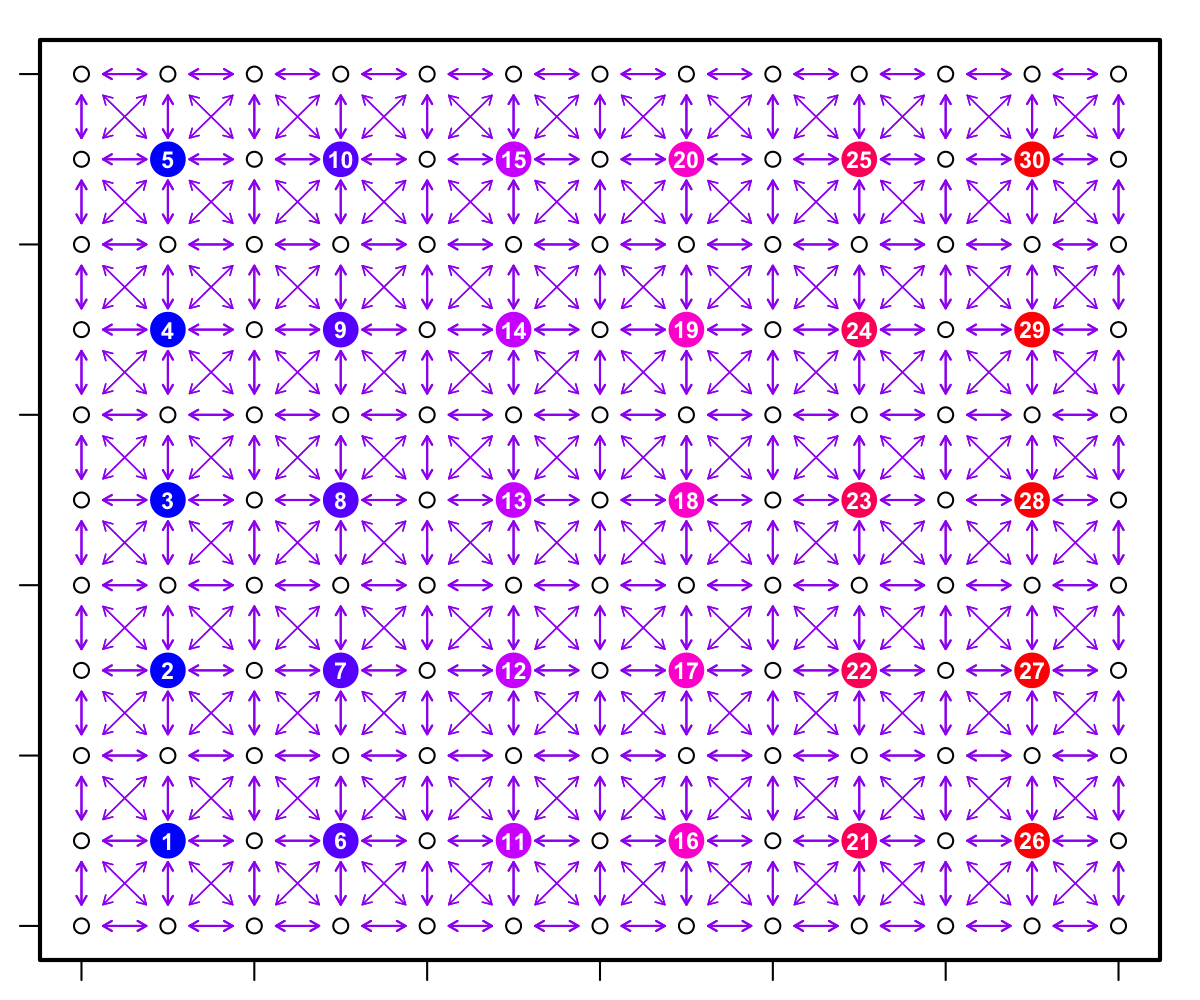
\includegraphics[width=3in,height=2.5in]{figs/sims/basic_lattice.png}}
		\subcaptionbox{Lattice with Barrier \label{barrier_lattice}}
			{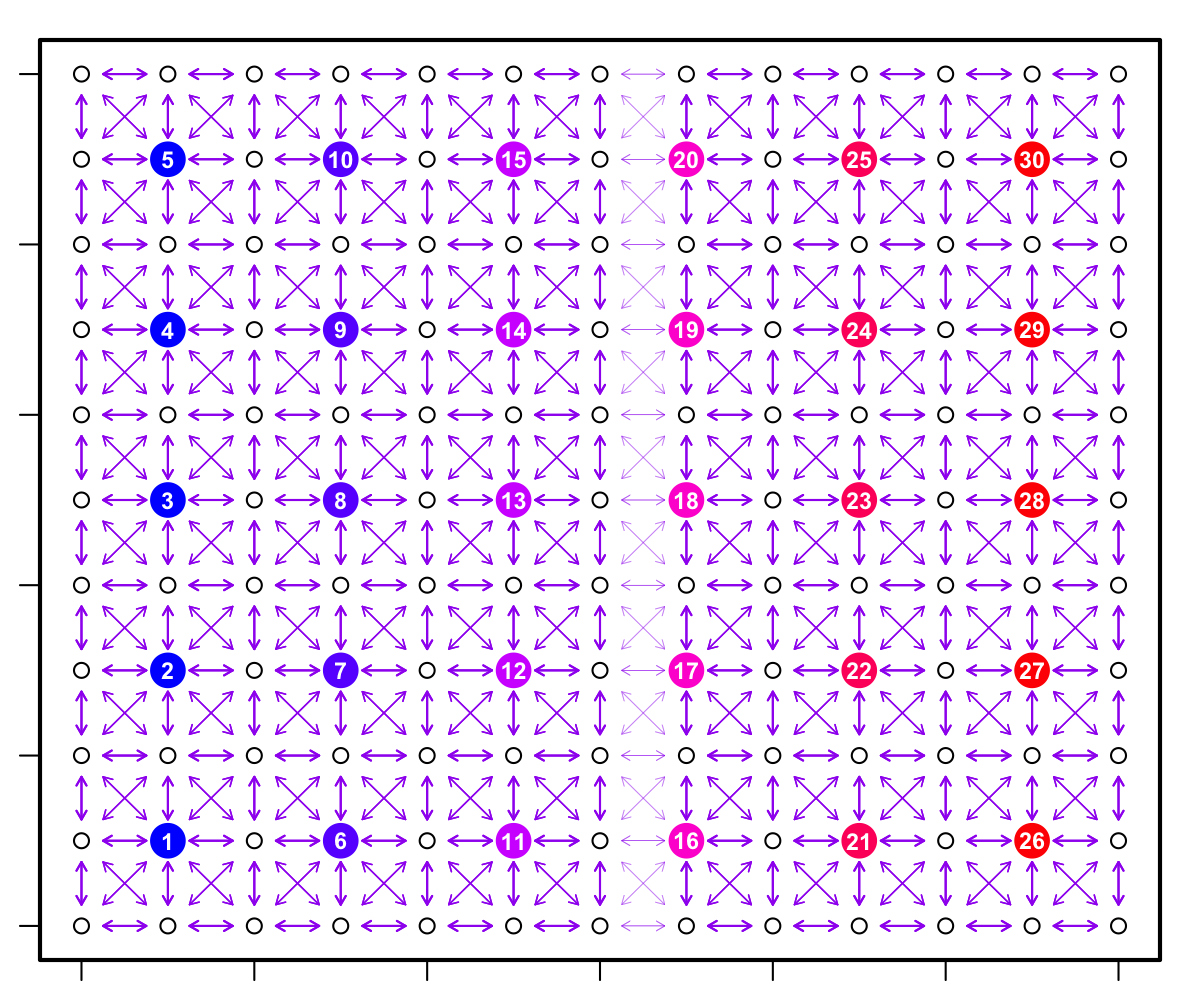
\includegraphics[width=3in,height=2.5in]{figs/sims/barrier_lattice.png}}
		\subcaptionbox{Lattice with Expansion Event \label{barrier_lattice}}
			{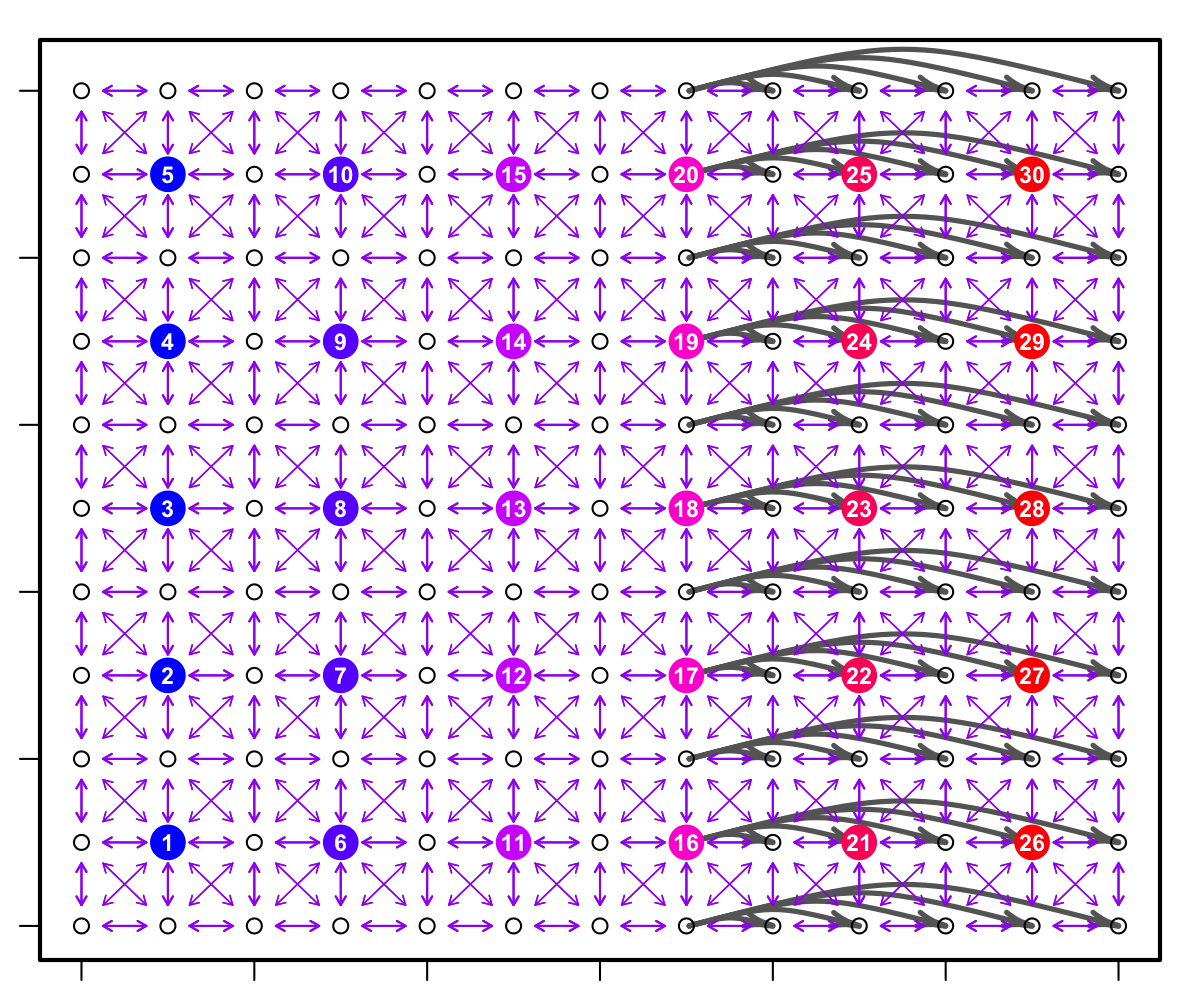
\includegraphics[width=3in,height=2.5in]{figs/sims/expansion_lattice.png}}
	\caption{Different simulation scenarios: (a) basic lattice; (b) lattice with a longitudinal barrier; (c) lattice with expansion event.}\label{sfig:sim_scenarios}
\end{figure}

\begin{figure}[ht!]
	\centering
		{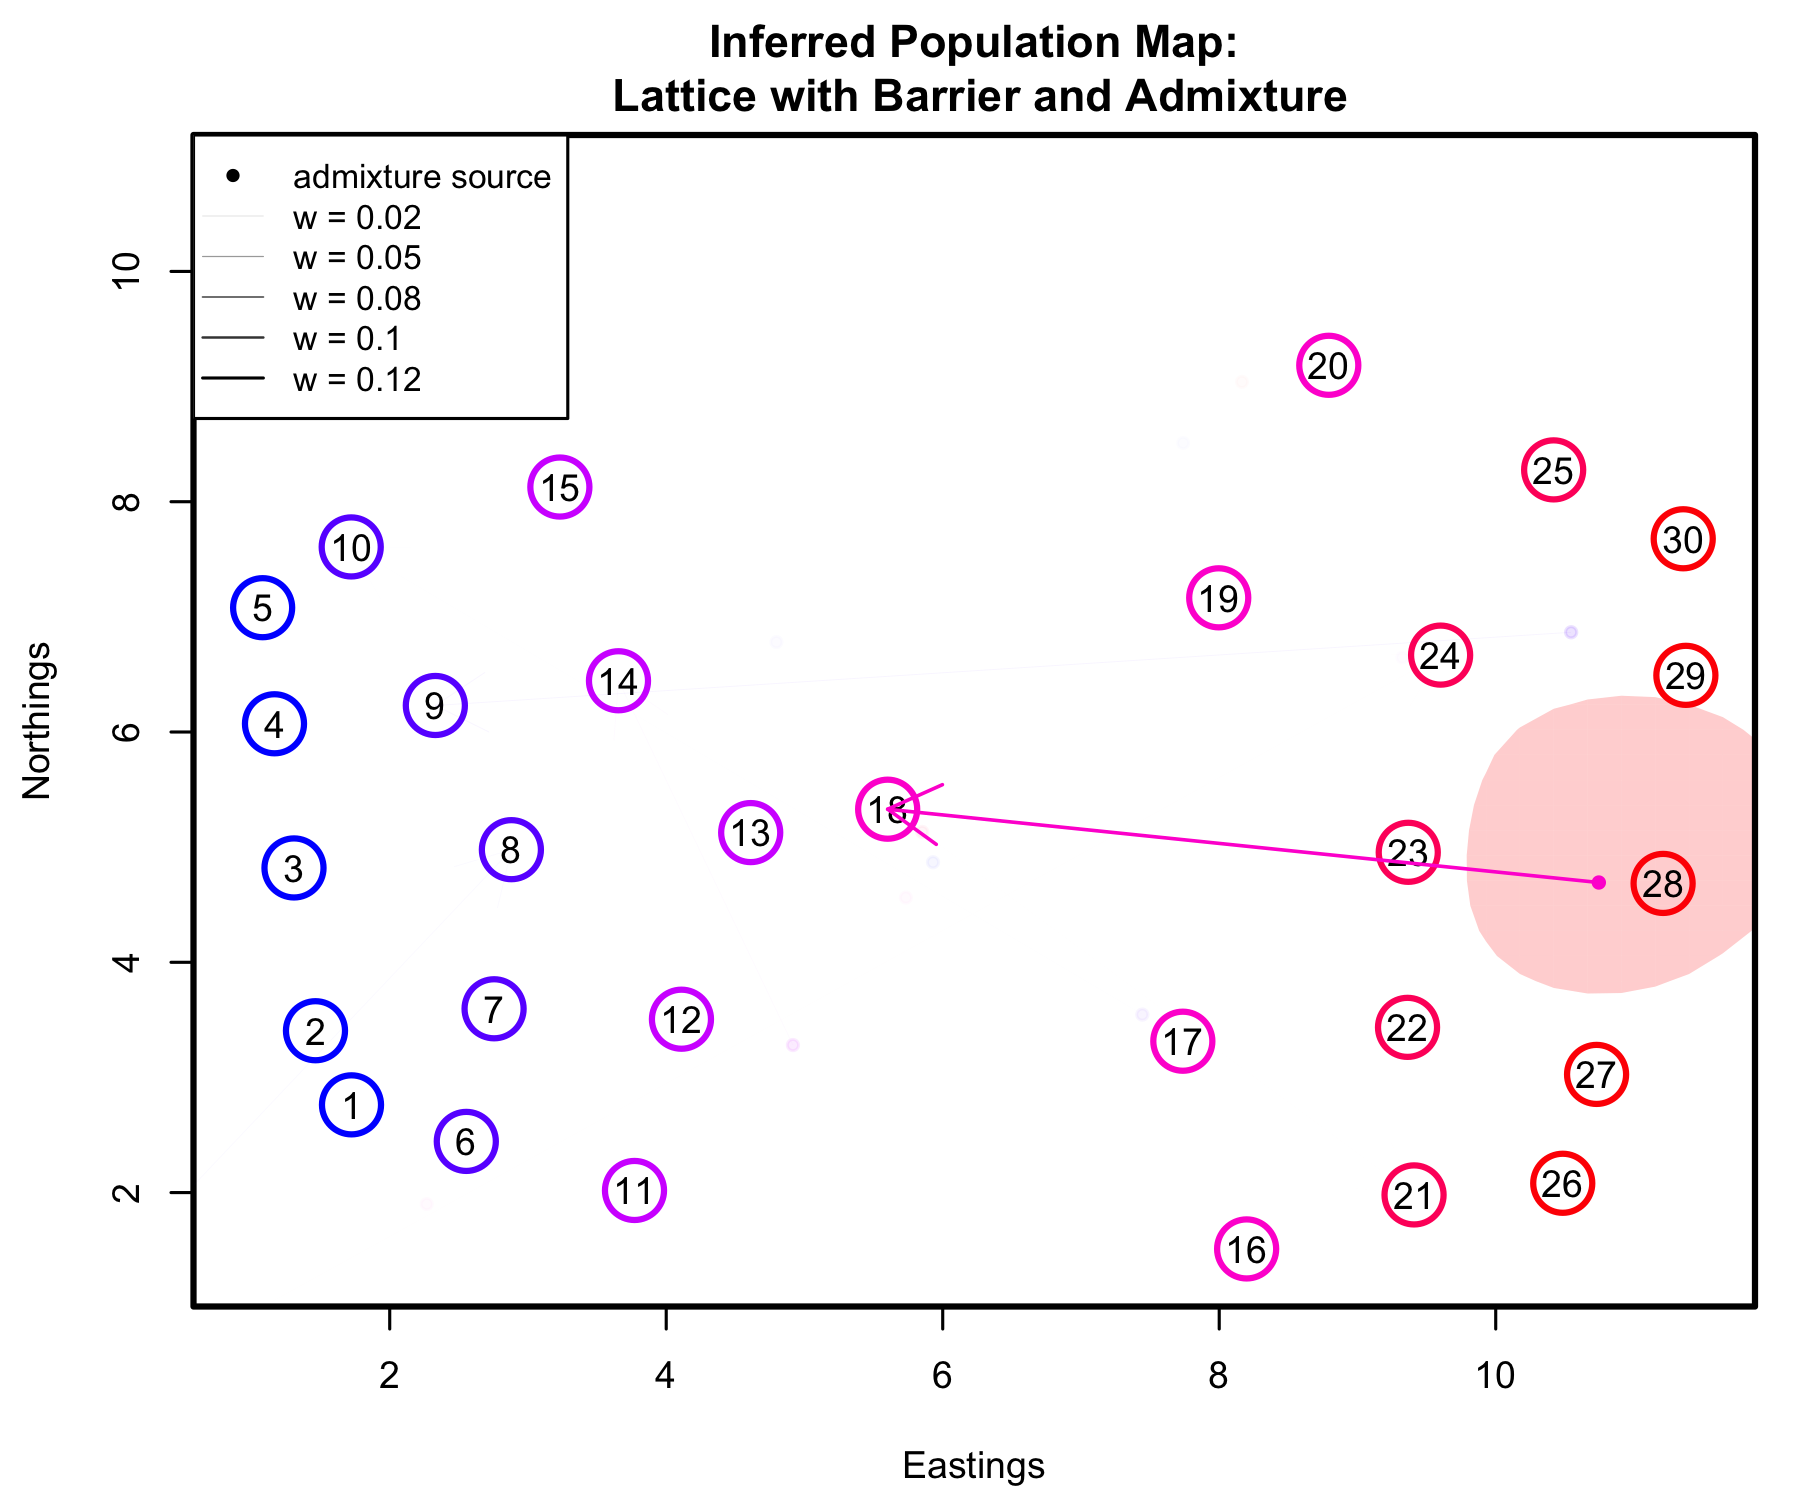
\includegraphics[width=2.4in,height=2in]{figs/sims/GeoGenMap_barr_inland_admixture_2.png}}
	\caption{credible interval of where population 23 draws admixture from.}
\label{sfig:barr_inland_ad_credset}
\end{figure}

\begin{figure}
	\centering
		\subcaptionbox{Likelihood \label{admix_prop_func_loc_lnl}}
			{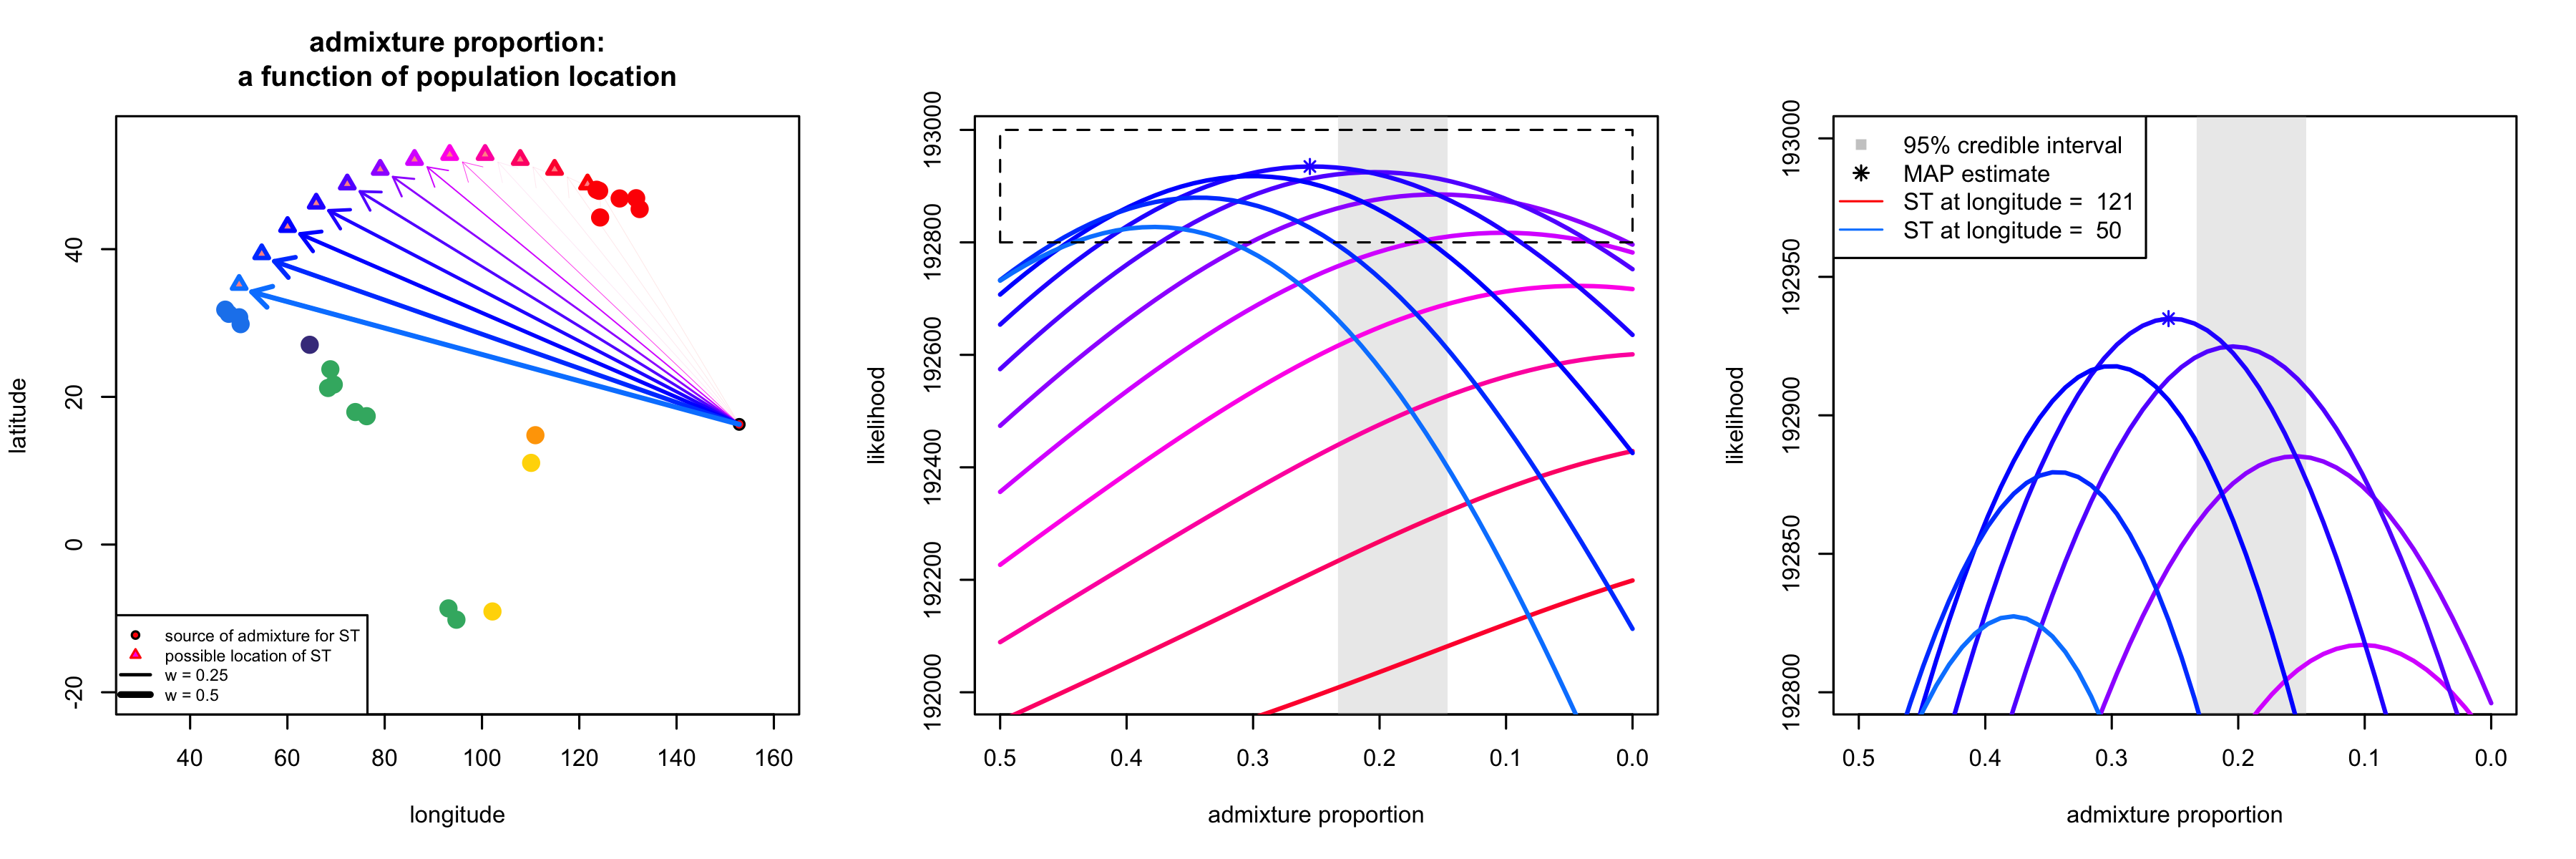
\includegraphics[width=6in,height=2in]{figs/warblers/admix_prop_func_loc_lnl.png}}
		\subcaptionbox{Posterior probability \label{admix_prop_func_loc_prob}}
			{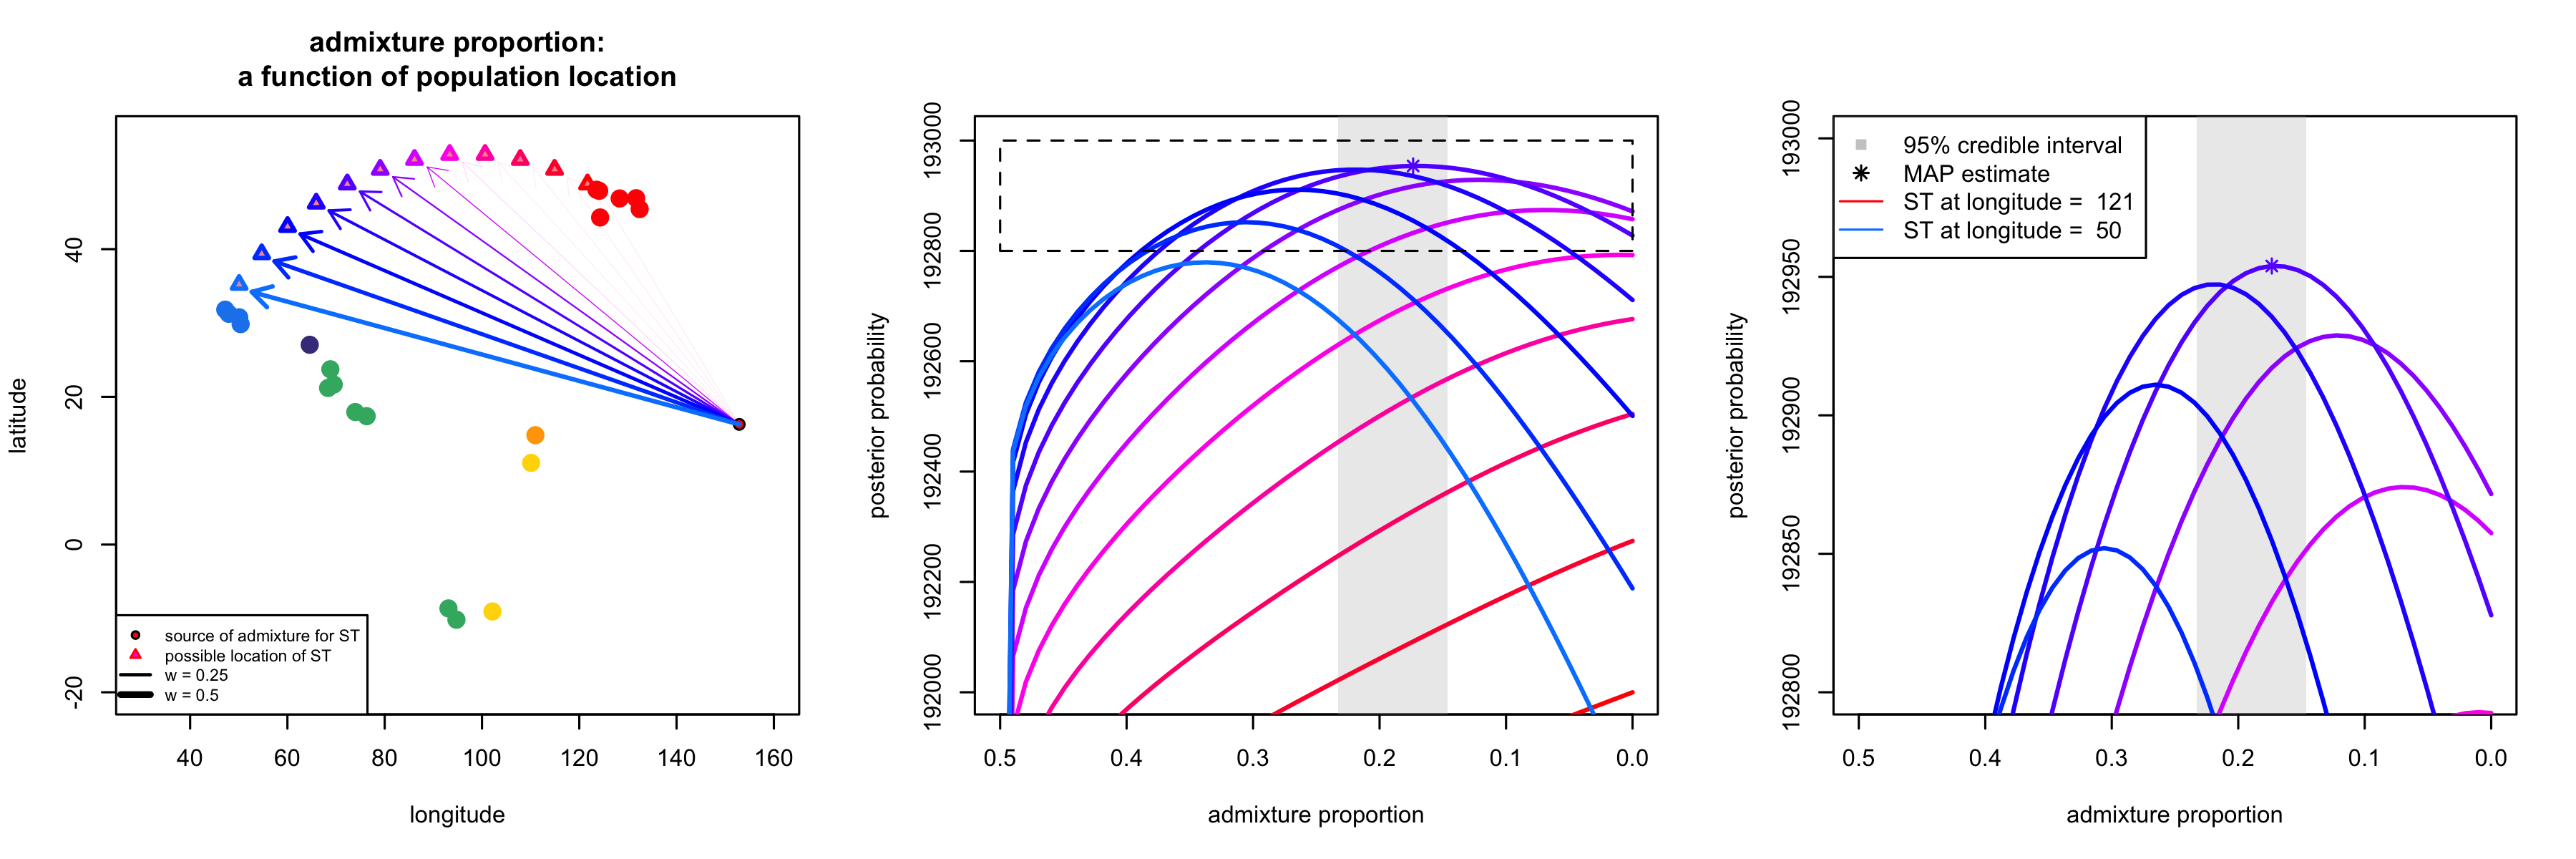
\includegraphics[width=6in,height=2in]{figs/warblers/admix_prop_func_loc_prob.png}}
	\caption{Likelihood surfaces for different placements of population ST between \textit{plumbeitarsus} and \textit{viridanus} clusters: (a) log likelihood surface; (b) posterior probability surface, incorporating the priors.}\label{sfig:admix_prop_func_loc}
\end{figure}

\begin{figure}
	\centering
		\subcaptionbox{All population pairs \label{warb_ind_dist_compare_allpairs}}
			{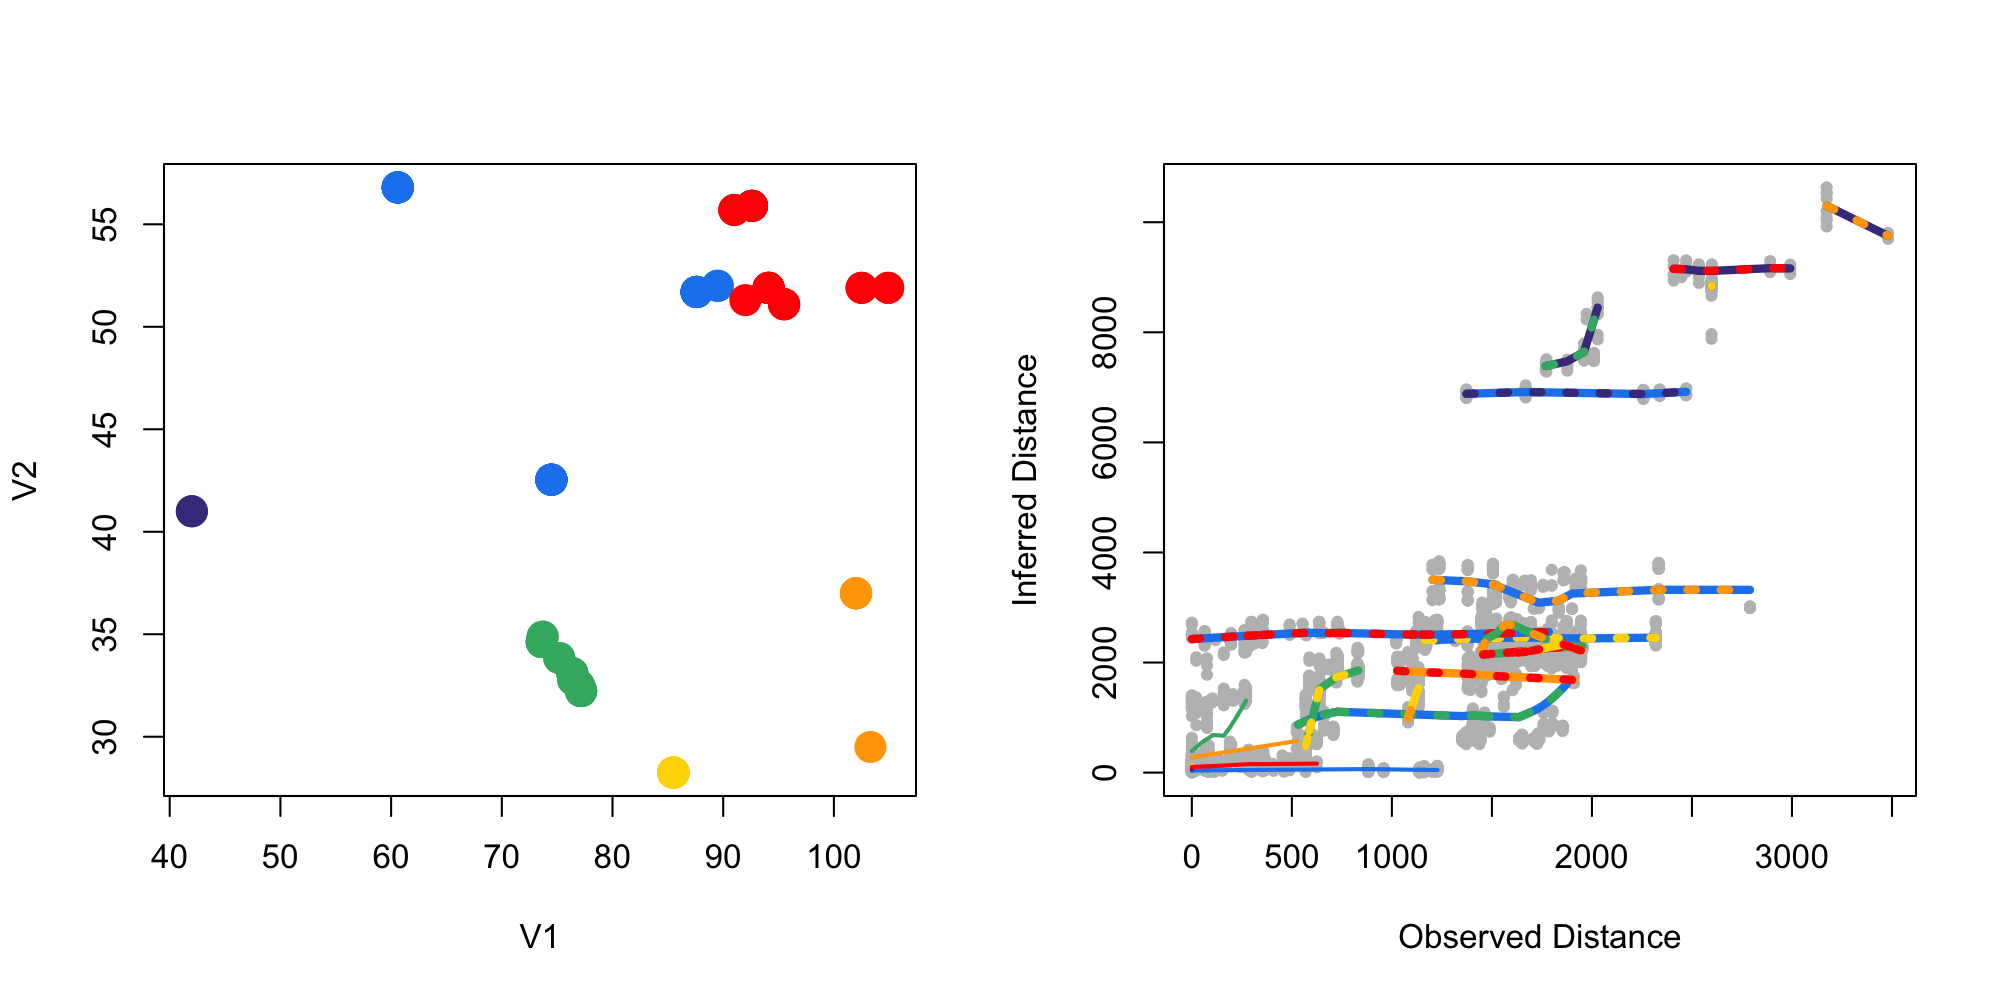
\includegraphics[width=6in,height=3in]{figs/warblers/warb_ind_dist_compare_allpairs.png}}
		\subcaptionbox{Just within population comparisons \label{warb_ind_dist_compare}}
			{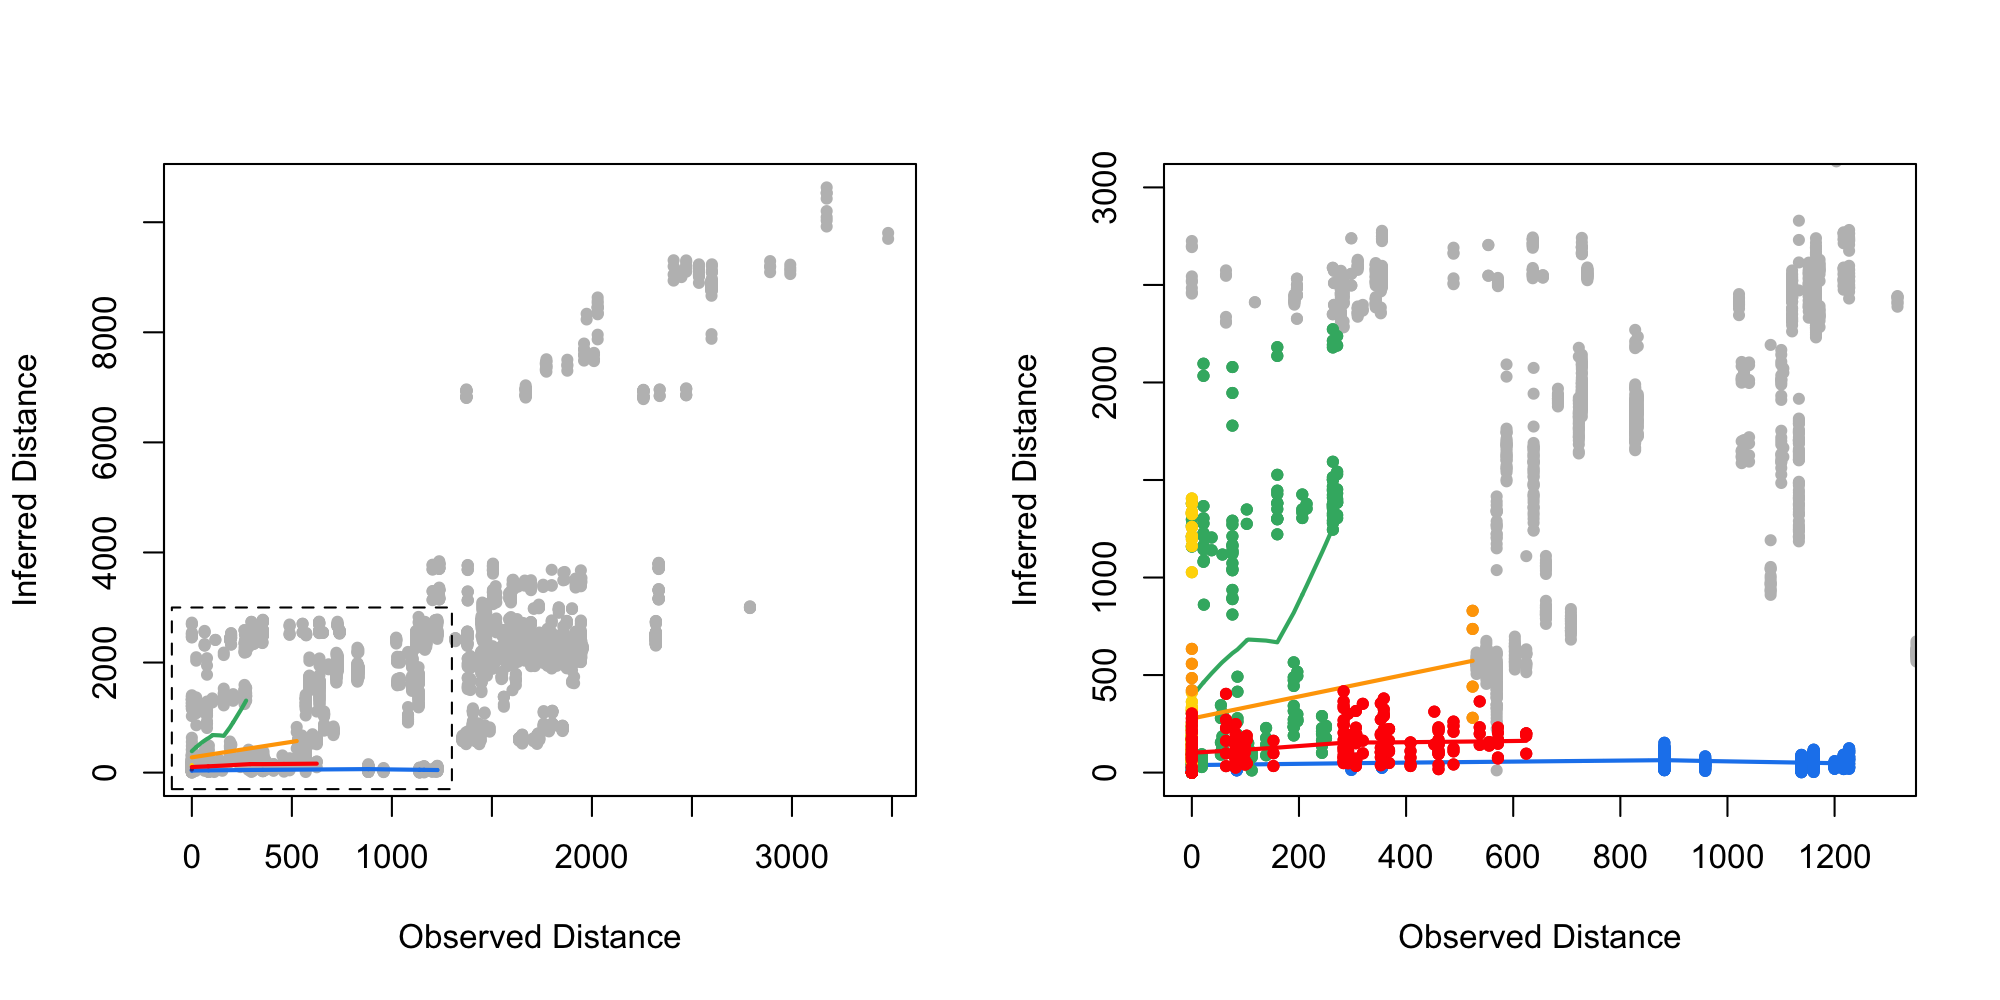
\includegraphics[width=6in,height=3in]{figs/warblers/warb_ind_dist_compare.png}}
	\caption{Comparing observed to estimated pairwise distance between warbler individuals, (a) between and (b) within subspecies populations.}\label{sfig:warb_ind_distcomp}
\end{figure}


\end{document}





%%%%%%%%%%%%%%%%%%%%%%%%%%%%%%%%
%	TEXT GRAVEYARD
%%%%%%%%%%%%%%%%%%%%%%%%%%%%%%%%


 in which we estimate the 2-dimensional configuration of populations that, along with a model of the decay of covariance in allele frequencies with distance, best describes their empirical patterns of genetic differentiation
 
\subsection*{Spatial Admixture Statistic}

\subsection*{Modeling Admixture}
where $f_{\ell,i}$ is the allele frequency in population $i$, $f_{\ell,j}$ is the allele frequency in population $j$, and $p$ is the admixture proportion, which varies between 0 and 1 and describes the extent to which populations $i$ and $j$ are contributing to the genetic make-up of population $k$.

 To infer the spatial context of this admixture, we allow each population a point in space, which we refer to as its source of admixture, from which it draws its admixture, and we model both the location of that source and the extent (proportion) of that admixture.  The observed allele frequencies in sampled populations are therefore a weighted average of the model-estimated allele frequencies at the geographic location of the sampled population and those at the coordinates of the source from which the observed population draws admixture.  That is, the observed allele frequencies in population $k$ are modeled as follows:
 \begin{equation}
 f_{k} = pf_{k'} + (1-p)f_{j},
 \end{equation}
 where $f_{k'}$ are the model-estimated allele frequencies across loci at the spatial location of population $k$ and $f_{j}$ are the model-estimated allele frequencies at the spatial location of the source of admixture $j$, from which population $k$ is drawing admixture in proportion $p$.  The admixture proportion $p$ is constrained to vary between 0 and 0.5, such that at least half of a population's genetic make-up must be determined by its geographic location.

 We re-introduce the population-specific variance terms on each diagonal element of this admixed covariance matrix.  The full expression for our admixed covariance function is below.
 \begin{alignat}{3}
 \label{eq:admixed_covariance_2}
 \Omega^{(*)}_{i,j} = (1-p_i)(1-p_j) \Omega_{i\;,\;j\;} \; \times&\\
 (p_i)(1-p_j) \Omega_{i^{(*)},\;j\;} \; \times   \notag&\\
 (p_j)(1-p_i) \Omega_{i\;,\;j^{(*)}} \; \times   \notag&\\
 (p_i)(p_j) \Omega_{i^{(*)},\;j^{(*)}} \; +   \notag&\\
 \delta_{i,j} \bar{S_k}^{-1} + \delta_{i,j} \eta_k \phantom{+} \notag&
 \end{alignat}

 where $I$ is the identity matrix, $\bar{S_k}$ is the mean sample size in population $k$ across all loci, and $\eta_k$ is the nugget estimated in population $k$.
